\documentclass[10pt, letterpaper]{article}

% Inhaltsverzeichnis für Pakettypen (nur für Übersicht im Header, wird nicht im Dokument angezeigt)
% 1. Seitenlayout und Ränder
% 2. Sprache und Zeichensatz
% 3. Mathematik und Theorem-Umgebungen
% 4. Eigene Makros
% 5. Diagramme und Grafiken
% 6. Tabellen und Aufzählungen
% 7. Inhaltsverzeichnis
% 8. Abschnittsüberschriften
% 9. Abstrakt-Umgebung
% 10. Todos/Notizen
% 11. Rahmen/Box-Umgebungen
% 12. Python-Integration
% 13. Literaturverwaltung
% 14. Hyperlinks
% 15. Absatzeinstellungen
% 16. Umgebungen
% 17  Graphik
% 18  Extra
% 00. Titel und Autor

% --- 1. Seitenlayout und Ränder ---
\usepackage[margin=3cm]{geometry}

% --- 2. Sprache und Zeichensatz ---
\usepackage[english]{babel}
\usepackage[T1]{fontenc}
\usepackage[utf8]{inputenc}

% --- 3. Mathematik und Theorem-Umgebungen ---
\usepackage{amsmath, amssymb, amsthm}
\usepackage{mathrsfs}
\DeclareMathOperator{\WF}{WF}

% --- 4. Eigene Makros ---
\usepackage{xcolor}
\newcommand{\SKP}{\langle\cdot,\cdot\rangle}
\newcommand{\R}{\mathbb{R}}
\newcommand{\N}{\mathbb{N}}
\newcommand{\Q}{\mathbb{Q}}
\newcommand{\Z}{\mathbb{Z}}
\newcommand{\C}{\mathbb{C}}
\newcommand{\entwurf}[1]{\textcolor{red}{#1}}

% --- 5. Diagramme und Grafiken ---
\usepackage{graphicx}
\usepackage{tikz}
\usetikzlibrary{decorations.pathreplacing, arrows.meta, positioning}
\usepackage{tikz-cd}

% --- 6. Tabellen und Aufzählungen ---
\usepackage{enumitem}
\setlist[itemize]{left=0.5cm}

\newenvironment{romanenum}[1][]
  {%
    \ifx&#1&
    \else
      \textbf{#1}\quad
    \fi
    \begin{enumerate}[label=\roman*)]
  }
  {%
    \end{enumerate}%
  }

% --- 7. Inhaltsverzeichnis ---
\usepackage{tocloft}
\renewcommand{\cftsecfont}{\footnotesize}
\renewcommand{\cftsubsecfont}{\footnotesize}
\renewcommand{\cftsubsubsecfont}{\footnotesize}
\renewcommand{\cftsecpagefont}{\footnotesize}
\renewcommand{\cftsubsecpagefont}{\footnotesize}
\renewcommand{\cftsubsubsecpagefont}{\footnotesize}
\usepackage{etoc}

% --- 8. Abschnittsüberschriften ---
\usepackage{titlesec}
\titleformat{\section}{\normalfont\large\bfseries}{\thesection}{1em}{}
\titleformat{\subsection}{\normalfont\normalsize\bfseries}{\thesubsection}{0.5em}{}
\titleformat{\subsubsection}{\normalfont\normalsize\bfseries}{\thesubsubsection}{0.5em}{}
\setcounter{secnumdepth}{4}

% --- 9. Abstrakt-Umgebung ---
\usepackage{changepage}
\renewenvironment{abstract}
  {
    \begin{adjustwidth}{1.5cm}{1.5cm}
    \small
    \textsc{Abstract. –}%
  }
  {
    \end{adjustwidth}
  }

% --- 10. Todos/Notizen ---
\usepackage{todonotes}

% --- 11. Rahmen/Box-Umgebungen ---
\usepackage{mdframed}
\usepackage{tcolorbox}
\colorlet{shadecolor}{gray!25}

\newenvironment{customTheorem}
  {\vspace{10pt}%
   \begin{mdframed}[
     backgroundcolor=gray!20,
     linewidth=0pt,
     innertopmargin=10pt,
     innerbottommargin=10pt,
     skipabove=\dimexpr\topsep+\ht\strutbox\relax,
     skipbelow=\topsep,
   ]}
  {\end{mdframed}
   \vspace{10pt}%
  }

% --- 12. Python-Integration ---
% (Deaktiviert in dieser Version, aktiviere bei Bedarf)
% \usepackage{pythontex}
% \usepackage[makestderr]{pythontex}

% --- 13. Literaturverwaltung ---
\usepackage{csquotes}
\usepackage[backend=biber, style=alphabetic, citestyle=alphabetic]{biblatex}
\addbibresource{bibliography.bib}

% --- 14. Hyperlinks ---
\usepackage{hyperref}
\hypersetup{
  colorlinks   = true,
  urlcolor     = blue,
  linkcolor    = blue,
  citecolor    = blue,
  frenchlinks  = true
}

% --- 15. Absatzeinstellungen ---
\usepackage[parfill]{parskip}
\sloppy

% --- 16. Umgebungen ---
\usepackage{thmtools}
\usepackage{tikz-cd}

\newcommand{\CustomHeading}[3]{%
  \par\medskip\noindent%
  \textbf{#1 #2} \textnormal{(#3)}.\enskip%
}

\newenvironment{DEF}[2]{\begin{unitbox}\CustomHeading{Definition}{#1}{#2}}{\end{unitbox}}
\newenvironment{PROP}[2]{\begin{unitbox}\CustomHeading{Proposition}{#1}{#2}}{\end{unitbox}}
\newenvironment{THEO}[2]{\begin{unitbox}\CustomHeading{Theorem}{#1}{#2}}{\end{unitbox}}
\newenvironment{LEM}[2]{\begin{unitbox}\CustomHeading{Lemma}{#1}{#2}}{\end{unitbox}}
\newenvironment{KORO}[2]{\begin{unitbox}\CustomHeading{Corollar}{#1}{#2}}{\end{unitbox}}
\newenvironment{REM}[2]{\begin{unitbox}\CustomHeading{Remark}{#1}{#2}}{\end{unitbox}}
\newenvironment{EXA}[2]{\begin{unitbox}\CustomHeading{Example}{#1}{#2}}{\end{unitbox}}
\newenvironment{STUD}[2]{\begin{unitbox}\CustomHeading{Study}{#1}{#2}}{\end{unitbox}}
\newenvironment{CONC}[2]{\begin{unitbox}\CustomHeading{Concept}{#1}{#2}}{\end{unitbox}}
\newenvironment{OTH}[2]{\begin{unitbox}\CustomHeading{Other}{#1}{#2}}{\end{unitbox}}
\newenvironment{EXE}[2]{\begin{unitbox}\CustomHeading{Exercise}{#1}{#2}}{\end{unitbox}}
\newenvironment{MOT}[2]{\begin{unitbox}\CustomHeading{Motivation}{#1}{#2}}{\end{unitbox}}
\newenvironment{PROOF}[2]{\begin{unitbox}\CustomHeading{Proof}{#1}{#2}}{\end{unitbox}}

% --- Unit Umgebung für Source-Inhalte ---
\usepackage{mdframed}
\newmdenv[
  linewidth=1pt,
  topline=false,
  bottomline=false,
  rightline=false,
  leftmargin=0cm,
  rightmargin=0cm,
  skipabove=10pt,
  skipbelow=10pt,
  innertopmargin=0.5\baselineskip,
  innerbottommargin=0.5\baselineskip,
  backgroundcolor=gray!10,
  linecolor=gray
]{unitbox}

\newenvironment{unit}[1]
  {\begin{unitbox}\textbf{Unit #1}\par\smallskip}
  {\end{unitbox}}

% --- 17. Graphik ---
\usepackage{graphicx}
\graphicspath{ {./images/} }
\usepackage[export]{adjustbox}

% --- 18. Extras ---
\usepackage{stmaryrd}
\usepackage{bbold}  % falls du athbb{1} nutzen willst

% --- 00. Titel und Autor ---
\title{Mein Titel}
\author{Tim Jaschik}
\date{\today}

\begin{document}

\maketitle
\rule{\textwidth}{0.5pt}
\begin{abstract}
Kurze Beschreibung …
\end{abstract}
\rule{\textwidth}{0.5pt}
\vspace{0.5cm}

\tableofcontents

\pagebreak

\section{Die Fundamentalgruppe}

Der Begriff des einfachen Zusammenhangs ist in mehreren Gebieten der Mathematik anzutreffen. Etwa besagt der Riemannsche Abbildungssatz, dass jedes einfach zusammenhängende Gebiet in $\mathbb{C}$ biholomorph zu $\mathbb{C}$ oder der Einheitsscheibe $\mathbb{E}=\{z \in \mathbb{C}:|z|<1\}$ ist. Etwas allgemeiner, jede einfach zusammenhängende Riemannsche Fläche (d.h. komplexe 1-dimensionale Mannigfaltigkeit) ist zu genau einer der Flächen $\mathbb{C}, \mathbb{E}$ oder $\mathbb{C} P^{1}$ biholomorph.

Ein Resultat aus der Theorie der Lie-Gruppen besagt, dass für eine einfach zusammenhängende Lie-Gruppe $G$ und jede weitere Lie-Gruppe $H$ die Abbildung die einem Lie-Gruppenhomomorphismus $G \rightarrow H$ den entsprechenden LieAlgebrenhomomorphismus $\mathfrak{g} \rightarrow \mathfrak{h}$ zuordnet bijektiv ist. Daher sind zwei einfach zusammenhängende Lie-Gruppen genau dann isomorph wenn es ihre LieAlgebren sind. Damit ist die Klassifikation der einfach zusammenhängenden LieGruppen auf die Klassifikation der Lie-Algebren zurückgeführt.

Eine vollständige einfach zusammenhängende $n$-dimensionale Riemannsche Mannigfaltigkeit mit konstanter Schnittkrümmung (o.B.d.A. $\kappa=-1,0,1$ ) ist isometrisch zu $\mathbb{R}^{n}$ (falls $\kappa=0$, euklidische Geometrie), $S^{n}$ (falls $\kappa=1$, sphärische Geometrie) oder $H^{n}$ (falls $\kappa=-1$, hyperbolische Geometrie).

Jedem (zusammenhängenden) topologischen Raum mit Basispunkt kann seine Fundamentalgruppe zugeordnet werden. Ihre Elemente sind Homotopieklassen geschlossener Wege beim Basispunkt, die Konkatenation von Wegen liefert die Gruppenstruktur. Ein zusammenhängender Raum ist einfach zusammenhängend genau dann, wenn seine Fundamentalgruppe trivial ist. Die Fundamentalgruppe liefert daher eine feine Abstufung zwischen den beiden Begriffen einfach zusammenhängend und nicht einfach zusammenhängend.

Die Fundamentalgruppe ist eine topologische Invariante, dh. homöomorphe zusammenhängende Räume haben isomorphe Fundamentalgruppen. Gelingt es von zwei Räumen die Fundamentalgruppen auszurechnen, und sind diese nicht isomorph, dann waren die beiden Räume nicht homöomorph. Da die Fundamentalgruppe eine Homotopieinvariante ist, lässt sich sogar schließen, dass die beiden Räume nicht einmal homotopieäquivalent sein können.

Mit Hilfe des Satzes von Seifert-van Kampen kann für einige interessante Räume die Fundamentalgruppe tatsächlich bestimmt werden. Etwa lassen sich die Fundamentalgruppen der geschlossenen Flächen berechnen, woraus dann folgt, dass geschlossene Flächen unterschiedlichen Geschlechts nicht homotopieäquivalent, und daher auch nicht homöomorph sind. Andere Beipiele kommen aus der Knotentheorie, haben die Komplemente zweier Knoten in $\mathbb{R}^{3}$ nicht-isomorphe Fundamentalgruppen, dann können die Knoten nicht äquivalent sein.

Die Fundamentalgruppe hat gute funktorielle Eigenschaften, stetigen Abbildungen zwischen Räumen entsprechen Homomorphismen zwischen ihren Fundamentalgruppen. Dies ist eine typische Situation in der algebraischen Topologie: topologischen Räumen werden algebraische Objekte (Gruppen, Ringe, ...)\\
zugeordnet, stetige Abbildungen entsprechen dabei in funktorieller Weise Homomorphismen zwischen diesen Objekte. Weitere Beipiele solcher topologischer Invarianten liefern die höheren Homotopiegruppen, die Homologiegruppen oder der Kohomologiering.

Die Berechnung der Fundamentalgruppe des Kreises, $\pi_{1}\left(S^{1}\right) \cong \mathbb{Z}$, führt rasch zu einem Beweis des Fundamentalsatzes der Algebra und auch zu einem Beweis des Browerschen Fixpunktsatzes für stetige Abbildungen $D^{2} \rightarrow D^{2}$. Sie erlaubt es auch für stetige Abbildungen $S^{1} \rightarrow S^{1}$ einen Abbildungsgrad zu definieren. Für stetig differenzierbare Abbildungen kann dieser auch als Integral geschrieben werden und liefert daher ein erstes einfaches Beispiel für den Zusammenhang zwischen Analysis und Topologie.

Der in diesem Kapitel behandelte Stoff ist Standardmaterial das sich in vielen Lehrbüchern findet. Die Darstellung hier orientiert sich eng an jenen in [4, Chapter 1] und [18, Kapitel 5], es seien aber auch [13], [15] und [19] erwähnt.






\pagebreak


\subsection{Elementare Eigenschaften der Fundamentalgruppe}

Es sei $X$ ein topologischer Raum. Weiters bezeichne $I:=[0,1] \subseteq \mathbb{R}$ das kompakte Einheitsintervall versehen mit der üblichen Teilraumtopologie. Unter einem Weg in $X$ verstehen wir eine stetige Abbildung $f: I \rightarrow X$. Wir nennen $f$ einen Weg von $f(0)$ nach $f(1)$. Stimmen die beiden Endpunkte eines Weges $f$ überein, dh. gilt $f(0)=x=f(1)$, dann wird $f$ ein geschlossener Weg oder eine Schleife bei $x$ genannt. Ist $x \in X$, dann bezeichnen wir mit $c_{x}: I \rightarrow X$ den konstanten Weg, $c_{x}(s):=x$.


\begin{DEF}{AT-H09-03-01}{Homotopie von Wegen in topologischen Räumen}
Unter einer Homotopie von Wegen in $X$ verstehen wir eine stetige Abbildung $H: I \times I \rightarrow X$, sodass $H(0, t)=x_{0}$ und $H(1, t)=x_{1}$ unabhängig von $t$ sind. Für jedes $t \in I$ ist dann $H_{t}: I \rightarrow X, H_{t}(s):=H(s, t)$, ein Weg von $H_{t}(0)=x_{0}$ nach $H_{t}(1)=x_{1}$.
\end{DEF}

\begin{DEF}{AT-H09-03-02}{Homotope Wege}
Zwei Wege $f, g: I \rightarrow X$ heißen homotop falls eine Homotopie von Wegen $H: I \times I \rightarrow X$ existiert, sodass $H_{0}=f$ und $H_{1}=g$, dh. $H(s, 0)=f(s)$ und $H(s, 1)=g(s)$ für alle $s \in I$. In diesem Fall wird $H$ eine Homotopie von $f$ nach $g$ genannt, und wir schreiben $f \simeq g$ oder $f \stackrel{H}{\simeq} g$. Um zu betonen, dass die Endpunkte fix sind, sprechen wir auch von einer Homotopie relativ Endpunkten und sagen $f$ ist homotop zu $g$ relativ Endpunkten.
\end{DEF}


I.1.1. Proposition. 

\begin{DEF}{AT-H09-03-03}{Homotopie relativ Endpunkt ist eine Äquivalenzrelation auf der Menge der Wege in $X$}
Homotop relativ Endpunkten zu sein ist eine Äquivalenzrelation auf der Menge der Wege in $X$.
\end{DEF}

Beweis. 

\begin{PROOF}{AT-H09-03-04}{P: Homotopie relativ Endpunkt ist eine Äquivalenzrelation auf der Menge der Wege in $X$}
Zur Reflexivität: Ist $f$ ein Weg in $X$, dann ist $H: I \times I \rightarrow X$, $H(s, t):=f(s)$, eine Homotopie relativ Endpunkten von $H_{0}=f$ nach $H_{1}=f$, also gilt $f \stackrel{H}{\simeq} f$. +

Zur Symmetrie: Sei also $f \stackrel{H}{\simeq} g$. Dann ist $G: I \times I \rightarrow X$, $G(s, t):=H(s, 1-t)$ eine Homotopie relativ Endpunkten von $G_{0}=H_{1}=g$ nach $G_{1}=H_{0}=f$, also gilt $g \stackrel{G}{\simeq} f$. 

Zur Transitivität: Seien also $f \stackrel{H^{\prime}}{\simeq} g$ und $g \stackrel{H^{\prime \prime}}{\simeq} h$.
Dann ist
$$
H: I \times I \rightarrow X, \quad H(s, t):= \begin{cases}H^{\prime}(s, 2 t) & \text { falls } 0 \leq t \leq 1 / 2 \\ H^{\prime \prime}(s, 2 t-1) & \text { falls } 1 / 2 \leq t \leq 1\end{cases}
$$
eine Homotopie relativ Endpunkten von $H_{0}=H_{0}^{\prime}=f$ nach $H_{1}=H_{1}^{\prime \prime}=h$, also gilt $f \stackrel{H}{\simeq} h$. Die Stetigkeit von $H$ folgt aus Lemma I.1.2 unten.
\end{PROOF}

\begin{DEF}{AT-H09-03-05}{Homotopieklassen}
Die Äquivalenzklassen der Äquivalenzrelation $\simeq$ heißen Homotopieklassen. Wir schreiben $[f]$ für die Homotopieklasse eines Weges $f$.
\end{DEF}


I.1.2. Lemma. 


\begin{LEM}{AT-H09-03-06}{Charakterisierung von Stetigkeit}
Es seien $X$ und $Y$ zwei topologische Räume und $f: Y \rightarrow X$ eine Abbildung. Weiters seien $A$ und $B$ zwei abgeschlossene Teilmengen von $Y$, sodass $Y=A \cup B$. In dieser Situation gilt: $f$ ist genau dann stetig, wenn die Einschränkungen $\left.f\right|_{A}: A \rightarrow X$ und $\left.f\right|_{B}: B \rightarrow X$ beide stetig sind.
\end{LEM}

Beweis. 

\begin{PROOF}{AT-H09-03-07}{P: Charakterisierung von Stetigkeit}
Mit $f$ sind natürlich auch die Einschränkungen $\left.f\right|_{A}$ und $\left.f\right|_{B}$ stetig. Es bleibt daher zu zeigen, dass aus der Stetigkeit der Einschränkungen auch die Stetigkeit von $f$ folgt. Sei dazu $C$ eine abgeschlossene Teilmenge von $X$ und $D:=f^{-1}(C) \subseteq Y$. Es ist zu zeigen, dass $D$ in $Y$ abgeschlossen ist. Aus der Stetigkeit von $\left.f\right|_{A}$ folgt, dass $D \cap A=\left.f\right|_{A} ^{-1}(D)$ abgeschlossen in $A$ ist. Da $A$ in $Y$ abgeschlossen ist folgt, dass $D \cap A$ auch in $Y$ abgeschlossen ist. Ebenso folgt aus der Stetigkeit von $\left.f\right|_{B}$ und der Abgeschlossenheit von $B$, dass $D \cap B$ abgeschlossen in $Y$ ist. Also ist auch ihre Vereinigung $(D \cap A) \cup(D \cap B)=D \cap(A \cup B)=D$ abgeschlossen in $Y$.
\end{PROOF}


I.1.3. Beispiel (Reparametrisierung). Ist $f: I \rightarrow X$ ein Weg und $\varphi: I \rightarrow I$ stetig mit $\varphi(0)=0$ und $\varphi(1)=1$, dann gilt $f \circ \varphi \simeq f$. Es ist nämlich $H$ : $I \times I \rightarrow X, H(s, t):=f((1-t) \varphi(s)+t s)$ eine Homotopie relativ Endpunkten von $H_{0}=f \circ \varphi$ nach $H_{1}=f$. Beachte, dass $(1-t) \varphi(s)+t s$ stets in $I$ liegt und $H$ daher wohldefiniert ist.\\


I.1.4. Beispiel. Es sei $X \subseteq \mathbb{R}^{n}$ eine konvexe Teilmenge und $f, g: I \rightarrow X$ zwei Wege mit $f(0)=g(0)$ und $f(1)=g(1)$. Dann gilt $f \simeq g$, denn $H: I \times I \rightarrow X$, $H(s, t):=(1-t) f(s)+t g(s)$, ist eine Homotopie relativ Endpunkten von $H_{0}=$ $f$ nach $H_{1}=g$. Beachte, dass wegen der Konvexität von $X$ diese Homotopie tatsächlich Werte in $X$ hat.

\begin{DEF}{AT-H09-03-08}{Produktwege in topologischen Räumen}
Es sei $X$ ein topologischer Raum. Sind $f$ und $g$ zwei Wege in $X$ mit $f(1)=$ $g(0)$, dann ist
$$
f g: I \rightarrow X, \quad(f g)(s):= \begin{cases}f(2 s) & \text { falls } 0 \leq s \leq 1 / 2 \\ g(2 s-1) & \text { falls } 1 / 2 \leq s \leq 1\end{cases}
$$
ein Weg von $f(0)$ nach $g(1)$. Er wird der Produktweg, die Konkatenation oder auch Zusammensetzung von $f$ und $g$ genannt.
\end{DEF}


I.1.5. Lemma. 

\begin{LEM}{AT-H09-03-09}{Homotopie von Produktwegen}
Es seien $f_{0}, f_{1}, g_{0}$ und $g_{1}$ Wege in $X$, sodass $f_{0} \simeq f_{1}, g_{0} \simeq g_{1}$, $f_{0}(1)=g_{0}(0)$ und daher auch $f_{1}(1)=g_{1}(0)$. Dann gilt $f_{0} g_{0} \simeq f_{1} g_{1}$.
\end{LEM}

Beweis. 

\begin{PROOF}{AT-H09-03-10}{P: Homotopie von Produktwegen}
Sind $F: I \times I \rightarrow X$ und $G: I \times I \rightarrow X$ Homotopien von Wegen mit $f_{0} \stackrel{F}{\simeq} f_{1}$ und $g_{0} \stackrel{G}{\simeq} g_{1}$, dann definiert
$$
H: I \times I \rightarrow X, \quad H(s, t):= \begin{cases}F(2 s, t) & \text { falls } 0 \leq s \leq 1 / 2 \\ G(2 s-1, t) & \text { falls } 1 / 2 \leq s \leq 1\end{cases}
$$
eine Homotopie relativ Endpunkten von $H_{0}=f_{0} g_{0}$ nach $H_{1}=f_{1} g_{1}$. Die Stetigkeit von $H$ folgt wieder aus Lemma I.1.2.
\end{PROOF}


I.1.6. Lemma. 



\begin{LEM}{AT-H09-03-11}{Assoziativität der Homotopie von Produktwegen}
Sind $f, g$ und $h$ drei Wege in $X$ mit $f(1)=g(0)$ und $g(1)=$ $h(0)$, dann gilt $(f g) h \simeq f(g h)$.
\end{LEM}


Beweis. 


\begin{PROOF}{AT-H09-03-12}{Assoziativität der Homotopie von Produktwegen}
$(fg)h$ ist eine Reparametrisierung von $f(g h)$, denn es gilt $(f g) h=$ $(f(g h)) \circ \varphi$ mit
$$
\varphi: I \rightarrow I, \quad \varphi(s):= \begin{cases}2 \mathrm{~s} & \text { falls } 0 \leq s \leq 1 / 4 \\ \mathrm{~s}+1 / 4 & \text { falls } 1 / 4 \leq s \leq 1 / 2 \\ \mathrm{~s} / 2+1 / 2 & \text { falls } 1 / 2 \leq s \leq 1\end{cases}
$$
Aus Beispiel I.1.3 folgt daher $(f g) h \simeq f(g h)$.
\end{PROOF}





I.1.7. Lemma. 

\begin{LEM}{AT-H09-03-13}{Existenz eines neutralen Elements für Homotopie}
Es sei $f$ ein Weg in $X$ und $x:=f(0), y:=f(1)$. Dann gilt für die Konkatenationen mit den konstanten Wegen $f c_{y} \simeq f$ sowie $c_{x} f \simeq f$.
\end{LEM}

Beweis. 

\begin{PROOF}{AT-H09-03-14}{Existenz eines neutralen Elements für Homotopie}
Der Weg $f c_{y}$ ist eine Reparametrisierung von $f$, denn es gilt $f c_{y}=$ $f \circ \varphi$ mit
$$
\varphi: I \rightarrow I, \quad \varphi(s):= \begin{cases}2 s & \text { falls } 0 \leq s \leq 1 / 2, \text { und } \\ 1 & \text { falls } 1 / 2 \leq s \leq 1\end{cases}
$$
Aus Beispiel I.1.3 folgt daher $f c_{y} \simeq f$. Analog lässt sich $c_{x} f \simeq f$ zeigen.
Für einen Weg $f: I \rightarrow X$ ist $\bar{f}: I \rightarrow X, \bar{f}(s):=f(1-s)$, ein Weg von $f(1)$ nach $f(0)$. Er wird als der zu $f$ inverse Weg bezeichnet.
\end{PROOF}



I.1.8. Lemma. 


\begin{LEM}{AT-H09-03-15}{Existenz von inversen Elements für Homotopie}
Es sei $f$ ein Weg in $X$ und $x:=f(0), y:=f(1)$. Dann gilt $f \bar{f} \simeq c_{x}$ und $\bar{f} f \simeq c_{y}$.
\end{LEM}

Beweis. 

\begin{PROOF}{AT-H09-03-16}{Existenz von inversen Elements für Homotopie}
Es ist
$$
H: I \times I \rightarrow X, \quad H(s, t):= \begin{cases}f(2 s) & \text { falls } 0 \leq s \leq t / 2 \\ f(t) & \text { falls } t / 2 \leq s \leq 1-t / 2 \\ f(2-2 s) & \text { falls } 1-t / 2 \leq s \leq 1\end{cases}
$$
eine Homotopie relativ Endpunkten von $H_{0}=c_{x}$ nach $H_{1}=f \bar{f}$. Die Stetigkeit von $H$ folgt wieder aus Lemma I.1.2. Analog lässt sich $\bar{f} f \simeq c_{y}$ zeigen.
\end{PROOF}




\begin{DEF}{AT-H09-03-17}{Menge aller Homotopieklassen relativ Endpunkt}
Sei $X$ ein topologischer Raum und $x_{0} \in X$ ein Basispunkt. Mit $\pi_{1}\left(X, x_{0}\right)$ bezeichnen wir die Menge aller Homotopieklassen geschlossener Wege bei $x_{0}$, genauer
$$
\pi_{1}\left(X, x_{0}\right):=\left\{\text { Wege } f: I \rightarrow X \text { mit } f(0)=x_{0}=f(1)\right\} / \simeq
$$
wobei $\simeq$ die oben besprochene Äquivalenzrelation der Homotopie relativ Endpunkten bezeichnet. Ist $f$ ein Weg in $X$ mit $f(0)=x_{0}=f(1)$ dann schreiben wir $[f]$ für seine Äquivalenzklasse in $\pi_{1}\left(X, x_{0}\right)$.
\end{DEF}


Nach Lemma I.1.5 definiert die Konkatenation von Wegen eine Multiplikation
$$
\pi_{1}\left(X, x_{0}\right) \times \pi_{1}\left(X, x_{0}\right) \rightarrow \pi_{1}\left(X, x_{0}\right), \quad([f],[g]) \mapsto[f][g]:=[f g]
$$
die nach Lemma I.1.6 assotiativ ist, $([f][g])[h]=[f]([g][h])$. Die Äquivalenzklasse des konstanten Weges $c_{x_{0}}$ ist nach Lemma I.1.7 neutrales Element dieser Multiplikation, $[f]\left[c_{x_{0}}\right]=[f]=\left[c_{x_{0}}\right][f]$. Nach Lemma I.1.8 gilt weiters $[f][\bar{f}]=\left[c_{x_{0}}\right]=$ $[\bar{f}][f]$. Zusammenfassend erhalten wir


I.1.9. Proposition. 

\begin{PROP}{AT-H09-03-18}{Fundamentalgruppe $(\pi_1(X,x_0),\cdot)$ ist eine Gruppe bzgl Produktwegen}
Die Konkatenation von Wegen definiert auf $\pi_{1}\left(X, x_{0}\right)$ eine Gruppenstruktur, $[f][g]=[f g]$. Das neutrale Element wird durch den konstanten Weg $c_{x_{0}}$ repräsentiert, $1=\left[c_{x_{0}}\right]$. Das zu $[f]$ inverse Element wird durch den inversen Weg repräsentiert, $[f]^{-1}=[\bar{f}]$.
\end{PROP}



I.1.10. Definition (Fundamentalgruppe). 

\begin{DEF}{AT-H09-03-19}{Fundamentalgruppe $(\pi_1(X,x_0),\cdot)$ relativ Endpunkt}
Die Gruppe $\pi_{1}\left(X, x_{0}\right)$ wird als die Fundamentalgruppe oder erste Homotopiegruppe von $X$ beim Basispunkt $x_{0}$ bezeichnet.
\end{DEF}


I.1.11. Bemerkung. 

Die Gruppe $\pi_{1}\left(X, x_{0}\right)$ ist i.A. nicht kommutativ und wird daher i.A. multiplikativ notiert. Insbesondere schreiben wir $1 \in \pi_{1}\left(X, x_{0}\right)$ für das neutrale Element und $\sigma^{-1}$ für das Inverse von $\sigma \in \pi_{1}\left(X, x_{0}\right)$. Ist die Fundamentalgruppe abelsch, so wird sie manchmal auch additiv geschrieben. Ist sie trivial, dh. besteht sie nur aus dem neutralen Element $\pi_{1}\left(X, x_{0}\right)=\{1\}$, dann wird dies üblicherweise durch die additive Schreibweise $\pi_{1}\left(X, x_{0}\right)=0$ ausgedrückt.


I.1.12. Beispiel. Ist $X \subseteq \mathbb{R}^{n}$ eine konvexe Teilmenge und $x_{0} \in X$ so gilt $\pi_{1}\left(X, x_{0}\right)=0$, siehe Beispiel I.1.4.


\begin{DEF}{AT-H09-03-20}{Punktierte Räume}
Unter einem punktierten Raum verstehen wir ein Paar ( $X, x_{0}$ ) wobei $X$ ein topologischer Raum und $x_{0} \in X$ ein Basispunkt ist. Punktierte Räume werden auch als Räume mit Basispunkt bezeichnet. Jedem punktierten Raum ( $X, x_{0}$ ) haben wir in Definition I.1.10 seine Fundamentalgruppe $\pi_{1}\left(X, x_{0}\right)$ zugeordnet.
\end{DEF}

\begin{DEF}{AT-H09-03-21}{Abbildung punktierter Räume}
Sind ( $X, x_{0}$ ) und ( $Y, y_{0}$ ) zwei punktierte Räume und ist $\varphi: X \rightarrow Y$ stetig mit $\varphi\left(x_{0}\right)=y_{0}$, dann nennen wir $\varphi$ eine Abbildung punktierter Räume oder auch basispunkterhaltende stetige Abbildung und schreiben $\varphi:\left(X, x_{0}\right) \rightarrow\left(Y, y_{0}\right)$. Ist $\psi:\left(Y, y_{0}\right) \rightarrow\left(Z, z_{0}\right)$ eine weitere Abbildung punktierter Räume, dann ist auch die Komposition $\psi \circ \varphi:\left(X, x_{0}\right) \rightarrow\left(Z, z_{0}\right)$ eine Abbildung punktierter Räume. Die identische Abbildung $\operatorname{id}_{\left(X, x_{0}\right)}:\left(X, x_{0}\right) \rightarrow\left(X, x_{0}\right)$ ist basispunkterhaltend. Unter einem Homöomorphismus punktierter Räume verstehen wir einen basispunkterhaltenden Homöomorphismus.
\end{DEF}


I.1.13. Proposition. 

\begin{PROP}{AT-H09-03-22}{Induzierter G-Homomorphismus zwischen Fundamentalgruppen von punktierten topologischen Räumen}
Eine Abbildung punktierter Räume $\varphi:\left(X, x_{0}\right) \rightarrow$ ( $Y, y_{0}$ ) induziert einen Gruppenhomomorphismus
$$
\varphi_{*}: \pi_{1}\left(X, x_{0}\right) \rightarrow \pi_{1}\left(Y, y_{0}\right), \quad \varphi_{*}([f]):=[\varphi \circ f] .
$$
Ist $\psi:\left(Y, y_{0}\right) \rightarrow\left(Z, z_{0}\right)$ eine weitere Abbildung punktierter Räume, dann gilt 
$$(\psi \circ \varphi)_{*}=\psi_{*} \circ \varphi_{*} \qquad \left(\operatorname{id}_{\left(X, x_{0}\right)}\right)_{*}=\operatorname{id}_{\pi_{1}\left(X, x_{0}\right)}$$
\end{PROP}



Beweis. 



\begin{PROOF}{AT-H09-03-23}{P: Induzierter G-Homomorphismus zwischen Fundamentalgruppen von punktierten topologischen Räumen}
Sei also $\varphi:\left(X, x_{0}\right) \rightarrow\left(Y, y_{0}\right)$ eine Abbildung punktierter Räume, und $f$ eine Schleife bei $x_{0}$. Dann ist $\varphi \circ f$ eine Schleife bei $y_{0}$. Sind $f_{0}, f_{1}$ zwei Schleife bei $x_{0}$ mit $f_{0} \xrightarrow{H} f_{1}$, so ist $\varphi \circ H: I \times I \rightarrow Y$ eine Homtopie von Wegen mit 
$$\varphi \circ f_{0} \stackrel{\varphi \circ H}{\simeq} \varphi \circ f_{1}$$ 
also 
$$\left[\varphi \circ f_{0}\right]=\left[\varphi \circ f_{1}\right] \in \pi_{1}\left(Y, y_{0}\right)$$ 
Dies zeigt, dass $\varphi_{*}$ wohldefiniert ist. 

Für zwei Schleifen $f, g$ bei $x_{0}$ gilt offensichtlich $\varphi \circ(f g)=(\varphi \circ f)(\varphi \circ g)$, also 
$$\varphi_{*}([f][g])=\varphi_{*}([f g])=[\varphi \circ(f g)]=[(\varphi \circ f)(\varphi \circ g)]=[\varphi \circ f][\varphi \circ g]=\varphi_{*}([f]) \varphi_{*}([g])$$ 
Dies zeigt, dass $\varphi_{*}$ ein Gruppenhomomorphismus ist. 

Weiters gilt 
$$(\psi \circ \varphi)_{*}([f])=[(\psi \circ \varphi) \circ f]=[\psi \circ(\varphi \circ f)]=\psi_{*}([\varphi \circ f])=\psi_{*}\left(\varphi_{*}([f])\right)$$ 
und daher $(\psi \circ \varphi)_{*}=\psi_{*} \circ \varphi_{*}$. 

Die Aussage $\left(\operatorname{id}_{\left(X, x_{0}\right)}\right)_{*}=\operatorname{id}_{\pi_{1}\left(X, x_{0}\right)}$ ist ebenso trivial.
\end{PROOF}


I.1.14. Proposition. 


\begin{PROP}{AT-H09-03-24}{Induzierter G-Isomorphismus zwischen Fundamentalgruppen von homöomorphen punktierten topologischen Räumen}
Ist $\varphi:\left(X, x_{0}\right) \rightarrow\left(Y, y_{0}\right)$ ein Homöomorphismus punktierter Räume, so ist die induzierte Abbildung $\varphi_{*}: \pi_{1}\left(X, x_{0}\right) \rightarrow \pi_{1}\left(Y, y_{0}\right)$ ein Isomorphismus.
\end{PROP}

Beweis. 

\begin{PROOF}{AT-H09-03-25}{P: Induzierter G-Isomorphismus zwischen Fundamentalgruppen von homöomorphen punktierten topologischen Räumen}
Es bezeichne $\varphi^{-1}:\left(Y, y_{0}\right) \rightarrow\left(X, x_{0}\right)$ die Umkehrabbildung. Aus Proposition I.1.13 erhalten wir $\left(\varphi^{-1}\right)_{*} \circ \varphi_{*}=\left(\varphi^{-1} \circ \varphi\right)_{*}=\left(\operatorname{id}_{X}\right)_{*}=\operatorname{id}_{\pi_{1}\left(X, x_{0}\right)}$ sowie $\varphi_{*} \circ\left(\varphi^{-1}\right)_{*}=\left(\varphi \circ \varphi^{-1}\right)_{*}=\left(\operatorname{id}_{Y}\right)_{*}=\operatorname{id}_{\pi_{1}\left(Y, y_{0}\right)}$. Daher sind $\varphi_{*}$ und $\left(\varphi^{-1}\right)_{*}$ zueinander inverse Gruppenisomorphismen.
\end{PROOF}


I.1.15. Bemerkung. 


\begin{REM}{AT-H09-03-26}{Induzierte G-Homomorphismen zwischen FG stimmen für Homöomorphismen nicht i.A. überein}
Sind $\varphi, \psi:\left(X, x_{0}\right) \rightarrow\left(Y, y_{0}\right)$ zwei Homöomorphismen punktierter Räume, dann stimmen die induzierten Isomorphismen $\varphi_{*}$ und $\psi_{*}$ i.A. nicht überein, siehe etwa Beispiel I.2.2 unten.
\end{REM}


I.1.16. Proposition. 

\begin{PROP}{AT-H09-03-27}{Induzierter G-Homomorphismus zwischen Fundamentalgruppen für Inklusion von WZSH-Komponente sind Isomorph}
Es sei ( $X, x_{0}$ ) ein punktierter Raum und es bezeichne $X_{0}$ die Wegzusammenhangskomponente von $x_{0}$. Dann induzierte die kanonische Inklusion $\left(X_{0}, x_{0}\right) \rightarrow\left(X, x_{0}\right)$ einen Isomorphismus $\pi_{1}\left(X_{0}, x_{0}\right) \cong \pi_{1}\left(X, x_{0}\right)$.
\end{PROP}

Beweis. 


\begin{PROOF}{AT-H09-03-28}{P: Induzierter G-Homomorphismus zwischen Fundamentalgruppen für Inklusion von WZSH-Komponente sind Isomorph}
Es bezeichne $\iota:\left(X_{0}, x_{0}\right) \rightarrow\left(X, x_{0}\right)$ die kanonische Inklusion und $\iota_{*}: \pi_{1}\left(X_{0}, x_{0}\right) \rightarrow \pi_{1}\left(X, x_{0}\right)$ den induzierten Homomorphismus.

Wir zeigen zunächst, dass $\iota_{*}$ surjektiv ist. Ist $f: I \rightarrow X$ eine Schleife bei $x_{0}$, dann liegt diese zur Gänze in $X_{0}$ und kann daher als Schleife $f^{\prime}: I \rightarrow X_{0}$ aufgefasst werden, $\iota \circ f^{\prime}=f$. Diese repräsentiert ein Element $\left[f^{\prime}\right] \in \pi_{1}\left(X_{0}, x_{0}\right)$ für das offensichtlich $\iota_{*}\left(\left[f^{\prime}\right]\right)=\left[\iota \circ f^{\prime}\right]=[f]$ gilt. Somit ist $\iota_{*}$ surjektiv.

Kommen wir nun zur Injektivität von $\iota_{*}$. Es seien $f^{\prime}, g^{\prime}: I \rightarrow X_{0}$ zwei Schleifen bei $x_{0}$ mit 
$$\iota_{*}\left(\left[f^{\prime}\right]\right)=\iota_{*}\left(\left[g^{\prime}\right]\right) \in \pi_{1}\left(X, x_{0}\right)$$ 
Dann existiert eine Homotopie relativ Endpunkten $H: I \times I \rightarrow X$ von $H_{0}=\iota \circ f^{\prime}$ nach $H_{1}=\iota \circ g^{\prime}$. Da $I \times I$ wegzusammenhängend ist, nimmt $H$ nur Werte in $X_{0}$ an, kann daher als Homotopie $H^{\prime}: I \times I \rightarrow X_{0}$ aufgefasst werden, $\iota \circ H^{\prime}=H$. 

Insbesondere gilt $\iota \circ H_{0}^{\prime}=H_{0}=\iota \circ f^{\prime}$ und $\iota \circ H_{1}^{\prime}=H_{1}=\iota \circ g^{\prime}$, aus der Injektivität von $\iota$ folgt daher $H_{0}^{\prime}=f^{\prime}$ und $H_{1}^{\prime}=g^{\prime}$. 

Wir erhalten $f^{\prime} \stackrel{H^{\prime}}{\simeq} g^{\prime}$, dh. $\left[f^{\prime}\right]=\left[g^{\prime}\right] \in \pi_{1}\left(X_{0}, x_{0}\right)$, also ist $\iota_{*}$ injektiv.
\end{PROOF}



Wir wollen uns nun überlegen wie die Fundamentalgruppe eines Produktraumes mit den Fundamentalgruppen der Faktoren zusammenhängt. Wir beginnen damit das Produkt punktierter Räume und das Produkt von Gruppen zu besprechen.

Sind ( $X, x_{0}$ ) und ( $Y, y_{0}$ ) zwei punktierte Räume, dann ist auch

$$
\left(X, x_{0}\right) \times\left(Y, y_{0}\right):=\left(X \times Y,\left(x_{0}, y_{0}\right)\right)
$$

ein punktierter Raum, der als das Produkt der punktierten Räume ( $X, x_{0}$ ) und $\left(Y, y_{0}\right)$ bezeichnet wird. Die Projektionen auf die beiden Komponenten liefern zwei Abbildungen punktierter Räume $p_{X}:\left(X, x_{0}\right) \times\left(Y, y_{0}\right) \rightarrow\left(X, x_{0}\right)$ und $p_{Y}:\left(X, x_{0}\right) \times\left(Y, y_{0}\right) \rightarrow\left(Y, y_{0}\right)$, die als kanonische Projektionen bezeichnet werden. Das Produkt punktierter Räume hat die folgende universelle Eigenschaft: Ist $\left(Z, z_{0}\right)$ ein weiterer punktierter Raum und sind $\varphi_{X}:\left(Z, z_{0}\right) \rightarrow\left(X, x_{0}\right)$ sowie $\varphi_{Y}:\left(Z, z_{0}\right) \rightarrow\left(Y, y_{0}\right)$ zwei Abbildungen punktierter Räume, dann existiert genau eine Abbildung punktierter Räume $\varphi:\left(Z, z_{0}\right) \rightarrow\left(X, x_{0}\right) \times\left(Y, y_{0}\right)$, sodass\\
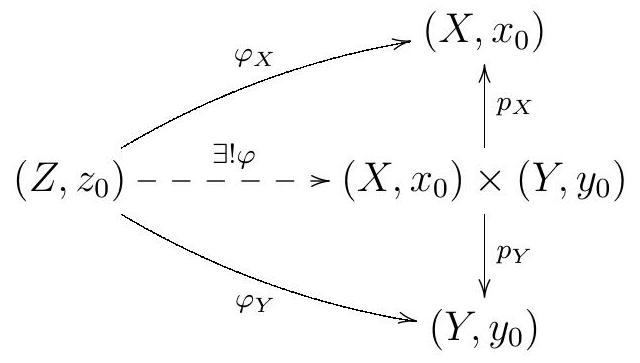
\includegraphics[max width=\textwidth]{2025_06_05_d7ed2bacd1e9ce1db1f0g-009} $p_{X} \circ \varphi=\varphi_{X}$ und $p_{Y} \circ \varphi=\varphi_{Y}$ gilt. Das nebenstehende kommutative Diagramm soll dies verdeutlichen. Diese Abbildung $\varphi$ ist durch $\varphi(x, y)=\left(\varphi_{X}(x), \varphi_{Y}(x)\right)$ gegeben und wird mit $\left(\varphi_{X}, \varphi_{Y}\right)$ bezeichnet.

Analog definieren wir das Produkt beliebig vieler punktierter Räume ( $X_{\alpha}, x_{\alpha}$ ), $\alpha \in A$, durch

$$
\prod_{\alpha \in A}\left(X_{\alpha}, x_{\alpha}\right):=\left(\prod_{\alpha \in A} X_{\alpha},\left(x_{\alpha}\right)_{\alpha \in A}\right)
$$

Dabei bezeichnet $\left(x_{\alpha}\right)_{\alpha \in A}$ den Punkt in $\prod_{\alpha \in A} X_{\alpha}$ mit Komponenten $x_{\alpha}$. Für jedes $\alpha \in A$ haben wir eine kanonische Projektion $p_{\alpha}: \prod_{\alpha^{\prime} \in A}\left(X_{\alpha^{\prime}}, x_{\alpha^{\prime}}\right) \rightarrow\left(X_{\alpha}, x_{\alpha}\right)$ mit folgender universellen Eigenschaft: Ist $\left(Z, z_{0}\right)$ ein punktierter Raum und sind $\varphi_{\alpha}:\left(Z, z_{0}\right) \rightarrow\left(X_{\alpha}, x_{\alpha}\right)$ Abbildungen punktierter Räume, $\alpha \in A$, dann existiert genau eine Abbildung punktierter Räume $\varphi:\left(Z, z_{0}\right) \rightarrow \prod_{\alpha \in A}\left(X_{\alpha}, x_{\alpha}\right)$, sodass $p_{\alpha} \circ \varphi=\varphi_{\alpha}$, für alle $\alpha \in A$. Diese Abbildung ist durch $\varphi(z)=\left(\varphi_{\alpha}(z)\right)_{\alpha \in A}$ gegeben und wird mit $\varphi=\left(\varphi_{\alpha}\right)_{\alpha \in A}$ bezeichnet. Durch diese universelle Eigenschaft ist das Produkt punktierter Räume zusammen mit den kanonischen Projektionen, bis auf kanonische Isomorphie eindeutig bestimmt.

Das Produkt von Gruppen besitzt eine analoge Eigenschaft. Sind $G$ und $H$ zwei Gruppen, dann ist $G \times H$ bezüglich komponentenweiser Multiplikation wieder eine Gruppe. Die beiden kanonischen Projektionen $p_{G}: G \times H \rightarrow G$ und $p_{H}: G \times H \rightarrow H$ sind Gruppenhomomorphismen. Das Produkt $G \times H$ hat die folgende universelle Eigenschaft: Sind $\varphi_{G}: K \rightarrow G$ und $\varphi_{H}$ : $K \rightarrow H$ zwei Gruppenhomomorphismen, dann existiert genau ein Gruppenhomomorphismus $\varphi: K \rightarrow G \times H$ mit $p_{G} \circ \varphi=\varphi_{G}$ und $p_{H} \circ \varphi=\varphi_{H}$. Dieser Homomorphi-\\
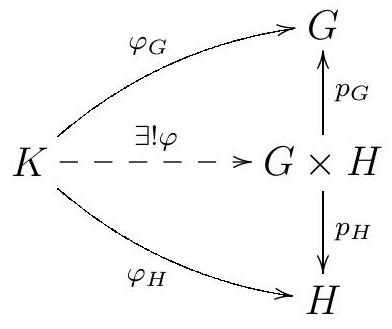
\includegraphics[max width=\textwidth]{2025_06_05_d7ed2bacd1e9ce1db1f0g-010} mus ist durch $\varphi(k)=\left(\varphi_{G}(k), \varphi_{H}(k)\right)$ gegeben und wird mit $\left(\varphi_{G}, \varphi_{H}\right)$ bezeichnet. Auch das Produkt beliebig vieler Gruppen $\prod_{\alpha \in A} G_{\alpha}$ hat diese Eigenschaft. Die kanonischen Projektionen $p_{\alpha}: \prod_{\alpha^{\prime} \in A} G_{\alpha^{\prime}} \rightarrow G_{\alpha}$ sind Gruppenhomomorphismen, und zu Gruppenhomomorphismen $\varphi_{\alpha}: K \rightarrow G_{\alpha}$, $\alpha \in A$, existiert genau ein Gruppenhomomorphismus $\varphi: K \rightarrow \prod_{\alpha \in A} G_{\alpha}$, sodass $p_{\alpha} \circ \varphi=\varphi_{\alpha}$, für alle $\alpha \in A$. Dieser Homomorphimus ist durch $\varphi(k)=\left(\varphi_{\alpha}(k)\right)_{\alpha \in A}$ gegeben und wird mit $\left(\varphi_{\alpha}\right)_{\alpha \in A}$ bezeichnet.

Nun aber zur Fundamentalgruppe des Produkts $\prod_{\alpha \in A}\left(X_{\alpha}, x_{\alpha}\right)$. Die kanonischen Projektionen $p_{\alpha}: \prod_{\alpha^{\prime} \in A}\left(X_{\alpha^{\prime}}, x_{\alpha^{\prime}}\right) \rightarrow\left(X_{\alpha}, x_{\alpha}\right)$ induzieren Gruppenhomomorphismen

$$
\left(p_{\alpha}\right)_{*}: \pi_{1}\left(\prod_{\alpha^{\prime} \in A}\left(X_{\alpha^{\prime}}, x_{\alpha^{\prime}}\right)\right) \rightarrow \pi_{1}\left(X_{\alpha}, x_{\alpha}\right), \quad[f] \mapsto\left[p_{\alpha} \circ f\right]
$$

Diese liefern einen Gruppenhomomorphismus

$$
\pi_{1}\left(\prod_{\alpha \in A}\left(X_{\alpha}, x_{\alpha}\right)\right) \rightarrow \prod_{\alpha \in A} \pi_{1}\left(X_{\alpha}, x_{\alpha}\right), \quad[f] \mapsto\left(\left[p_{\alpha} \circ f\right]\right)_{\alpha \in A^{*}}
$$

I.1.17. Proposition. Für punktierte Räume ( $X_{\alpha}, x_{\alpha}$ ), $\alpha \in A$, ist (I.1) ein Isomorphismus. Insbesondere gilt $\pi_{1}\left(X \times Y,\left(x_{0}, y_{0}\right)\right) \cong \pi_{1}\left(X, x_{0}\right) \times \pi_{1}\left(Y, y_{0}\right)$ für je zwei punktierte Räume ( $X, x_{0}$ ) und ( $Y, y_{0}$ ).

Beweis. Um die Surjektivität von (I.1) einzusehen, betrachten wir ein beliebiges Element $g \in \prod_{\alpha \in A} \pi_{1}\left(X_{\alpha}, x_{\alpha}\right)$, dh. $g=\left(\left[f_{\alpha}\right]\right)_{\alpha \in A}$ wobei $f_{\alpha}: I \rightarrow X_{\alpha}$ Schleifen bei $x_{\alpha}$ sind die Elemente $\left[f_{\alpha}\right] \in \pi_{1}\left(X_{\alpha}, x_{\alpha}\right)$ repräsentieren, $\alpha \in A$. Es ist dann $f:=\left(f_{\alpha}\right)_{\alpha \in A}: I \rightarrow \prod_{\alpha \in A} X_{\alpha}$ eine Schleife bei $\left(x_{\alpha}\right)_{\alpha \in A}$, definiert daher ein Element $[f] \in \pi_{1}\left(\prod_{\alpha \in A}\left(X_{\alpha}, x_{\alpha}\right)\right)$. Nach Konstruktion wird $[f]$ durch den Homomorphismus (I.1) auf $g$ abgebildet. Also ist (I.1) surjektiv.

Nun zur Injektivität von (I.1). Es seien $f, g: I \rightarrow \prod_{\alpha \in A} X_{\alpha}$ zwei Schleifen bei $\left(x_{\alpha}\right)_{\alpha \in A}$, sodass die davon repräsentierten Elemente $[f],[g] \in \pi_{1}\left(\prod_{\alpha \in A}\left(X_{\alpha}, x_{\alpha}\right)\right)$ dasselbe Bild unter (I.1) haben. Es gilt daher $\left[p_{\alpha} \circ f\right]=\left[p_{\alpha} \circ g\right] \in \pi_{1}\left(X_{\alpha}, x_{\alpha}\right)$, für alle $\alpha \in A$. Also existieren Homotopien relativ Endpunkten $H^{\alpha}: I \times I \rightarrow X_{\alpha}$ von $H_{0}^{\alpha}=p_{\alpha} \circ f$ nach $H_{1}^{\alpha}=p_{\alpha} \circ g, \alpha \in A$. Es definiert dann $H:=\left(H^{\alpha}\right)_{\alpha \in A}$ : $I \times I \rightarrow \prod_{\alpha \in A} X_{\alpha}$ eine Homotopie relativ Endpunkten von $f$ nach $g$. Damit ist $[f]=[g] \in \pi_{1}\left(\prod_{\alpha \in A}\left(X_{\alpha}, x_{\alpha}\right)\right)$ und (I.1) also injektiv.



Wir wenden uns nun der Frage zu, inwiefern die Fundamentalgruppe $\pi_{1}\left(X, x_{0}\right)$ eines Raumes $X$ vom Basispunkt $x_{0}$ abhängt.


I.1.18. Proposition. 

\begin{PROP}{AT-H09-03-29}{Induzierte G-Isomorphismus zwischen Fundamentalgruppen eines Raumes relativ wegzusammenhängenden Punkten}
Es sei $h: I \rightarrow X$ ein Weg und $x_{0}:=h(0), x_{1}:=h(1)$. Dann definiert
$$
\beta_{h}: \pi_{1}\left(X, x_{1}\right) \rightarrow \pi_{1}\left(X, x_{0}\right), \quad \beta_{h}([f]):=[h f \bar{h}]
$$
einen Isomorphismus von Gruppen, $\beta_{h}^{-1}=\beta_{\bar{h}}$.
\end{PROP}


Beweis. 

\begin{PROOF}{AT-H09-03-30}{P: Induzierte G-Isomorphismus zwischen Fundamentalgruppen eines Raumes relativ wegzusammenhängenden Punkten}
Nach den Beobachtungen am Beginn dieses Abschnitts ist $\beta_{h}$ wohldefiniert (Genaugenommen müssten wir hier Klammern setzten, $\beta_{h}([f])=[(h f) \bar{h}]$ oder $\beta_{h}([f])=$ $[h(f \bar{h})]$, nach Lemma I.1.6 stimmen die Homotopieklassen $[(h f) \bar{h}]$ und $[h(f \bar{h})]$ aber überein) und für $[f],[g] \in \pi_{1}\left(X, x_{1}\right)$ gilt 
$$\beta_{h}([f][g])=[h f g \bar{h}]=\left[h f c_{x_{1}} g \bar{h}\right]=[h f \bar{h} h g \bar{h}]=[h f \bar{h}][h g \bar{h}]=\beta_{h}([f]) \beta_{h}([g])$$ 
also ist $\beta_{h}$ ein Gruppenhomomorphismus. 

Verwenden wir noch die offensichtliche Tatsache $\overline{\bar{h}}=h$, so erhalten wir 
$$\left(\beta_{\bar{h}} \circ \beta_{h}\right)([f])=\beta_{\bar{h}}([h f \bar{h}])=[\bar{h} h f \bar{h} \overline{\bar{h}}]=[\bar{h} h f \bar{h} h]=\left[c_{x_{1}} f c_{x_{1}}\right]=[f]$$ 
Daher gilt $\beta_{\bar{h}} \circ \beta_{h}=\operatorname{id}_{\pi_{1}\left(X, x_{1}\right)}$. 

Ebenso lässt sich $\beta_{h} \circ \beta_{\bar{h}}=\operatorname{id}_{\pi_{1}\left(X, x_{0}\right)}$ zeigen, also sind $\beta_{h}$ und $\beta_{\bar{h}}$ zueinander inverse Gruppenisomorphismen.
\end{PROOF}



I.1.19. Bemerkung. 

\begin{REM}{AT-H09-03-31}{Fundamentalgruppen relativ zu Basispunkten in verschiedenen WZSH-Komponenten nicht i.A. isomorph}
Sind $x_{0}$ und $x_{1}$ zwei Basispunkte in $X$ die in derselben Wegzusammenhangskomponente von $X$ liegen, dann sind nach Proposition I.1.18 die Gruppen $\pi_{1}\left(X, x_{0}\right)$ und $\pi_{1}\left(X, x_{1}\right)$ isomorph. Für wegzusammenhängendes $X$ schreiben wir daher oft auch $\pi_{1}(X)$. Liegen $x_{0}$ und $x_{1}$ nicht in derselben Wegzusammenhangskomponente, dann dürfen wir uns i.A. keinerlei Relation zwischen den Gruppen $\pi_{1}\left(X, x_{0}\right)$ und $\pi_{1}\left(X, x_{1}\right)$ erwarten, vgl. Proposition I.1.16.
\end{REM}


I.1.20. Bemerkung. 

\begin{REM}{AT-H09-03-32}{Kanonizität des Connectors $\beta$ hängt von der Kommutativität der Fundamentalgruppen ab}
Der Isomorphismus $\beta_{h}$ aus Proposition I.1.18 hängt nur von der Homotopieklasse von $h$ ab, dh. aus $h \simeq h^{\prime}$ folgt $\beta_{h}=\beta_{h^{\prime}}$. 

Genauer, für zwei Wege $h, h^{\prime}$ von $x_{0}$ nach $x_{1}$ gilt $\beta_{h}=\beta_{h^{\prime}}$ genau dann, wenn $\left[h \bar{h}^{\prime}\right]$ im Zentrum - d.h. in $Z(G):=\{g \in G \mid \forall h \in G: g h=h g\}$, welches stehts ein abelscher Normalteiler ist (es gilt $Z(G)=G$ genau dann, wenn $G$ abelsch ist) - $Z\left(\pi_{1}\left(X, x_{0}\right)\right)$ der Fundamentalgruppe liegt. 

Ist $\pi_{1}\left(X, x_{0}\right)$ nicht abelsch, dann gilt 
$$Z\left(\pi_{1}\left(X, x_{0}\right)\right) \neq \pi_{1}\left(X, x_{0}\right)$$
und der in Proposition I.1.18 konstruierte Isomorphismus hängt tatsächlich von $[h] \mathrm{ab}$. 

Ist die Fundamentalgruppe nicht abelsch, erhalten wir daher keine kanonische Identifikation von $\pi_{1}\left(X, x_{0}\right)$ mit $\pi_{1}\left(X, x_{1}\right)$.
\end{REM}


I.1.21. Proposition. 

\begin{PROP}{AT-H09-03-33}{Äquivalenzcharakterisierungen von Eindeutiger Existenz einer Homotopieklasse von Wegen zwischen beliebigen Punkten}
Für einen topologischer Raum $X$ sind äquivalent:
\begin{enumerate}
\item Zu je zwei Punkten $x_{0}, x_{1} \in X$ gibt es genau eine Homotopieklasse von Wegen von $x_{0}$ nach $x_{1}$.
\item $X$ ist wegzusammenhängend, und für alle $x_{0} \in X$ gilt $\pi_{1}\left(X, x_{0}\right)=0$.
\item $X$ ist wegzusammenhängend, und es existiert $x_{0} \in X$ mit $\pi_{1}\left(X, x_{0}\right)=0$.
\end{enumerate}
\end{PROP}


Beweis. 


\begin{PROOF}{AT-H09-03-34}{P: Äquivalenzcharakterisierungen von Eindeutiger Existenz einer Homotopieklasse von Wegen zwischen beliebigen Punkten}
Die Äquivalenz (ii) $\Leftrightarrow$ (iii) folgt aus Proposition I.1.18. 

Nun zur Implikation (i) $\Rightarrow$ (ii): Da nach Voraussetzung mindestens eine Homotopieklasse von Wegen von $x_{0}$ nach $x_{1}$ existiert, muss $X$ wegzusammenhängend sein. Betrachten wir nun $x_{1}=x_{0}$, so folgt $\pi_{1}\left(X, x_{0}\right)=0$ aus der Annahme, dass höchstens eine Homotopieklasse von Wegen von $x_{0}$ nach $x_{1}$ existiert. 

Es bleibt (ii) $\Rightarrow$ (i) zu zeigen. Seien dazu $x_{0}, x_{1} \in X$. Aus dem Wegzusammenhang von $X$ folgt, dass es zumindest eine Homotopieklasse von Wegen von $x_{0}$ nach $x_{1}$ gibt. Sind $f, g: I \rightarrow X$ zwei Wege von $x_{0}$ nach $x_{1}$, dann ist $f \bar{g}$ eine Schleife bei $x_{0}$ die wegen $\pi_{1}\left(X, x_{0}\right)=0$ homotop zum konstanten Weg $c_{x_{0}}$ sein muss, $f \bar{g} \simeq c_{x_{0}}$. Es folgt 
$$f \simeq f c_{x_{1}} \simeq f(\bar{g} g) \simeq(f \bar{g}) g \simeq c_{x_{0}} g \simeq g$$ 
also kann es höchstens eine Homotopieklasse von Wegen von $x_{0}$ nach $x_{1}$ geben.
\end{PROOF}



I.1.22. Definition (Einfacher Zusammenhang). 

\begin{DEF}{AT-H09-03-35}{Einfach zusammenhängender typologischer Raum}
Ein topologischer Raum $X$ heißt einfach zusammenhängend, falls er die (äquivalenten) Bedingungen in Proposition I.1.21 erfüllt.
\end{DEF}



I.1.23. Beispiel. Jede konvexe Teilmenge von $\mathbb{R}^{n}$ ist einfach zusammenhängend, siehe Beispiel I.1.12. Beachte, dass konvexe Teilmengen offensichtlich wegzusammenhängend sind. Insbesonder sind $\mathbb{R}^{n}$, die abgeschlossenen Bälle $D^{n}:=$ $\left\{x \in \mathbb{R}^{n}:\|x\| \leq 1\right\}$ und die offenen Bälle $B^{n}:=\left\{x \in \mathbb{R}^{n}:\|x\|<1\right\}$ einfach zusammenhängend.\\


I.1.24. Beispiel. Das Produkt beliebig vieler einfach zusammenhängender Räume ist wieder einfach zusammenhängend, siehe Proposition I.1.17. Beachte, dass Produkte wegzusammenhängender Räume wieder wegzusammenhängend sind.

Für $n \in \mathbb{N}_{0}$ bezeichne $S^{n}:=\left\{x \in \mathbb{R}^{n+1}:\|x\|=1\right\}$ die $n$-dimensionale Einheitssphäre versehen mit der von $\mathbb{R}^{n+1}$ induzierten Teilraumtopologie. Beachte, dass $S^{n}$ abgeschlossen und beschränkt in $\mathbb{R}^{n+1}$ ist. Nach dem Satz von HeineBorel ist $S^{n}$ daher ein kompakter Raum. Etwa besteht $S^{0}=\{-1,1\}$ aus nur zwei Punkten. Die eindimensionale Sphäre können wir auch als Teilraum der komplexen Zahlen auffassen, $S^{1}=\{z \in \mathbb{C}:|z|=1\}$.


I.1.25. Beispiel. 

\begin{EXA}{AT-H09-03-36}{$S^n\backslash \{P\}$ ist EZSH}
$S^{n} \backslash\{P\}$ ist homöomorph zu $\mathbb{R}^{n}$ und daher einfach zusammenhängend, $P \in S^{n}, n \in \mathbb{N}_{0}$. Um dies einzusehen betrachten wir zunächst die Inversion mit Pol $P$,
$$
\nu_{P}: \mathbb{R}^{n+1} \backslash\{P\} \rightarrow \mathbb{R}^{n+1} \backslash\{P\}, \quad \nu_{P}(x):=P+\frac{2}{\|x-P\|^{2}}(x-P)
$$
Der Bildpunkt $\nu_{P}(x)$ liegt daher auf dem Halbstrahl von $P$ durch $x$ und es gilt $\|x-P\|\left\|\nu_{P}(x)-P\right\|=2$. Daraus folgt sofort $\nu_{P} \circ \nu_{P}=\operatorname{id}_{\mathbb{R}^{n+1} \backslash\{P\}}$, insbesondere ist $\nu_{P}$ ein Homöomorphismus. Weiters gilt
$$
\left\|\nu_{P}(x)\right\|^{2}=1+\frac{4\langle x, P\rangle}{\|x-P\|^{2}}
$$
und daher ist $\nu_{P}(x) \in S^{n}$ genau dann, wenn $x \in P^{\perp}=\left\{x \in \mathbb{R}^{n+1}:\langle x, P\rangle=0\right\}$. Die Einschränkung von $\nu_{P}$ liefert daher einen Homöomorphismus
$$
\varphi_{P}: P^{\perp} \rightarrow S^{n} \backslash\{P\}, \quad \varphi_{P}(x)=P+\frac{2}{\|x-P\|^{2}}(x-P)
$$
Dieser Homöomorphismus wird die stereographische Projektion mit Pol P genannt. Als Hyperebene in $\mathbb{R}^{n+1}$ ist $P^{\perp}$ homöomorph zu $\mathbb{R}^{n}$, daher ist auch $S^{n} \backslash\{P\}$ homöomorph zu $\mathbb{R}^{n}$. Nach Proposition I.1.14 und Beispiel I.1.23 ist daher $S^{n} \backslash\{P\}$ einfach zusammenhängend.
\end{EXA}


I.1.26. Satz. $S^{n}$ ist einfach zusammenhängend, falls $n \geq 2$.

Beweis. Bezeichne mit $N:=(0, \ldots, 0,1) \in S^{n}$ den Nordpol und mit $x_{0}:=$ $S:=(0, \ldots, 0,-1) \in S^{n}$ den Südpol. Weiters betrachte die offenen Teilmengen $U:=S^{n} \backslash\{N\}$ und $V:=S^{n} \backslash\{S\}$. Nach Beispiel I.1.25 ist $\pi_{1}\left(U, x_{0}\right)=0$, es genügt daher zu zeigen, dass die von der kanonischen Inklusion $\iota$ : $\left(U, x_{0}\right) \rightarrow\left(S^{n}, x_{0}\right)$ induzierte Abbildung $\iota_{*}: \pi_{1}\left(U, x_{0}\right) \rightarrow \pi_{1}\left(S^{n}, x_{0}\right)$ surjektiv ist. Sei dazu $f: I \rightarrow S^{n}$ eine Schleife bei $x_{0}$. Es ist zu zeigen, dass $f$ homotop relativ Endpunkten zu einer Schleife in $U$ ist. Da $\{U, V\}$ eine offene Überdeckung von $S^{n}$ ist, bilden auch die beiden Mengen $f^{-1}(U)$ und $f^{-1}(V)$ eine offene Überdeckung des Intervalls $I$. Da $I$ kompakt ist, existieren $0=s_{0}<s_{1}<\cdots<s_{m}=1$, sodass für jedes $i=1, \ldots, m$ entweder $f\left(\left[s_{i-1}, s_{i}\right]\right) \subseteq U$ oder $f\left(\left[s_{i-1}, s_{i}\right]\right) \subseteq V$ gilt, siehe Lemma I.1.28 unten. Durch Weglassen gewisser $s_{i}$ können wir erreichen, dass $f\left(s_{i}\right) \neq N$, für jedes $0 \leq i \leq m$, denn ist $f\left(s_{i}\right)=N$ dann muss $f\left(\left[s_{i-1}, s_{i}\right]\right) \subseteq V$ und $f\left(\left[s_{i}, s_{i+1}\right]\right) \subseteq V$ gelten. Betrachte die reparametrisierten Einschränkungen $f_{i}: I \rightarrow S^{n}, f_{i}(s):=f\left((1-s) s_{i-1}+s s_{i}\right), i=1,2, \ldots, m$. Nach Beispiel I.1.3 gilt dann $f \simeq f_{1} f_{2} \cdots f_{m}$, wobei wir wieder auf die Klammersetzung verzichten, da sie für die Aussage unwesentlich ist, vgl. Lemma I.1.6. Es genügt nun zu zeigen, dass jedes $f_{i}$ homotop relativ Endpunkten zu einem Weg in $U$ ist, denn dann ist auch $f$ homotop relativ Endpunkten zu einer Schleife in $U$, siehe Lemma I.1.5. Für die $i$ mit $f\left(\left[s_{i-1}, s_{i}\right]\right) \subseteq U$ ist nichts zu zeigen. Betrachten wir also ein $i$ mit $f\left(\left[s_{i-1}, s_{i}\right]\right) \subseteq V$, dh. $f_{i}(I) \subseteq V$. Die stereographischen Projektion $\varphi_{S}: \mathbb{R}^{n}=S^{\perp} \rightarrow S^{n} \backslash\{S\}=V$ aus Beispiel I.1.25 ist ein Homöomorphismus mit $\varphi_{S}(0)=N$. Also ist $\varphi_{S}^{-1} \circ f_{i}: I \rightarrow \mathbb{R}^{n}$ ein Weg in $\mathbb{R}^{n}$ und es gilt $\left(\varphi_{S}^{-1} \circ f_{i}\right)(0) \neq 0 \neq\left(\varphi_{S}^{-1} \circ f_{i}\right)(1)$, denn $f\left(s_{i}\right) \neq N$. Da $n \geq 2$ finden wir einen Weg $g_{i}: I \rightarrow \mathbb{R}^{n} \backslash\{0\}$ mit $g_{i}(0)=\left(\varphi_{S}^{-1} \circ f_{i}\right)(0)$ und $g_{i}(1)=\left(\varphi_{S}^{-1} \circ f_{i}\right)(1)$. Nach Konstruktion ist $\varphi_{S} \circ g_{i}$ ein Weg in $V \backslash\{N\} \subseteq U$. Da $\mathbb{R}^{n}$ einfach zusammenhängend ist, sind die beiden Wege $\varphi_{S}^{-1} \circ f_{i}$ und $g_{i}$ homotop relativ Endpunkten in $\mathbb{R}^{n}$, siehe Proposition I.1.21, also sind auch $f_{i}$ und $\varphi_{S} \circ g_{i}$ homotop relativ Endpunkten in $V \subseteq S^{n}$.\\

I.1.27. Beispiel. Für $n_{i} \geq 2$ ist $S^{n_{1}} \times \cdots \times S^{n_{k}}$ einfach zusammenhängend, siehe Satz I.1.26 und Beispiel I.1.24

Im Beweis von Satz I.1.26 haben wir von der Lebesguesche Überdeckungszahl Gebrauch gemacht, und wollen daher dieses elementare Resultat kurz wiederholen.


I.1.28. Lemma (Überdeckungszahl von Lebesgue). Es sei ( $X, d$ ) ein kompakter metrischer Raum und $\mathcal{U}$ eine offene Überdeckung von $X$. Dann existiert $\varepsilon>0$, sodass jeder Ball mit Radius $\varepsilon$ zur Gänze in einer der Überdeckungsmengen von $\mathcal{U}$ enthalten ist. Genauer, für jedes $x \in X$ existiert $U \in \mathcal{U}$ mit $B_{\varepsilon}(x) \subseteq U$, wobei $B_{\varepsilon}(x):=\{y \in X: d(x, y)<\varepsilon\}$ den offenen Ball mit Mittelpunkt $x$ und Radius $\varepsilon$ bezeichnet.

Beweis. Da $\mathcal{U}$ eine offene Überdeckung von $X$ bildet, existiert zu jedem $x \in X$ ein $r_{x}>0$ und $U_{x} \in \mathcal{U}$ mit $B_{2 r_{x}}(x) \subseteq U_{x}$. Die Bälle $B_{r_{x}}(x)$ bilden eine offene Überdeckung von $X$. Wegen der Kompaktheit von $X$ überdecken schon endlich viele davon ganz $X$, dh. $B_{r_{x_{1}}}\left(x_{1}\right) \cup \cdots \cup B_{r_{x_{n}}}\left(x_{n}\right)=X$ für gewisse $x_{1}, \ldots, x_{n} \in X$. Wir zeigen nun, dass $\varepsilon:=\min \left\{r_{x_{1}}, \ldots, r_{x_{n}}\right\}>0$ die gewünschte Eigenschaft besitzt. Sei dazu $x \in X$. Wähle $1 \leq i \leq n$ mit $x \in B_{r_{i}}\left(x_{i}\right)$. Aus der Dreiecksungleichung folgt $B_{r_{i}}(x) \subseteq B_{2 r_{i}}\left(x_{i}\right)$, und daher $B_{\varepsilon}(x) \subseteq B_{r_{i}}(x) \subseteq$ $B_{2 r_{i}}\left(x_{i}\right) \subseteq U_{x_{i}}$. Also liegt $B_{\varepsilon}(x)$ zur Gänze in der Überdeckungsmenge $U_{x_{i}}$.\\



\pagebreak


\subsection{Die Fundamentalgruppe des Kreises}


Wir wollen in diesen Abschnitt die Fundamentalgruppe von $S^{1}:=\{z \in \mathbb{C}:|z|=1\}$ bestimmen. Als Basispunkt verwenden wir $x_{0}:=1 \in S^{1}$. Für $n \in \mathbb{Z}$ betrachten wir den Weg

$$
\omega_{n}: I \rightarrow S^{1}, \quad \omega_{n}(s):=e^{2 \pi \mathbf{i} n s}=\cos (2 \pi n s)+\mathbf{i} \sin (2 \pi n s)
$$

Da $\omega_{n}(0)=\omega_{n}(1)=1$ ist jedes $\omega_{n}$ eine Schleife bei $1 \in S^{1}$ und definiert daher eine Homotopieklasse $\left[\omega_{n}\right] \in \pi_{1}\left(S^{1}, 1\right)$.\\




I.2.1. Satz. 

Die Abbildung $\phi: \mathbb{Z} \rightarrow \pi_{1}\left(S^{1}, 1\right), \phi(n):=\left[\omega_{n}\right]$, siehe (I.2), ist ein Isomorphismus von Gruppen, $\pi_{1}\left(S^{1}\right) \cong \mathbb{Z}$.


I.2.2. Beispiel. Für $k \in \mathbb{Z}$ betrachte die Basispunkt erhaltende Abbildung $p_{k}:\left(S^{1}, 1\right) \rightarrow\left(S^{1}, 1\right), p(z):=z^{k}$. Wir wollen nun den induzierten Homomorphismus $\left(p_{k}\right)_{*}: \pi_{1}\left(S^{1}, 1\right) \rightarrow \pi_{1}\left(S^{1}, 1\right)$ bestimmen. Genauer wollen wir zeigen, dass nebenstehendes Diagramm kommutiert, wobei $\phi: \mathbb{Z} \rightarrow \pi_{1}\left(S^{1}, 1\right)$ den Isomorphismus aus Satz I.2.1 bezeichent und $\mathbb{Z} \xrightarrow{\cdot k} \mathbb{Z}$ der durch Multiplikation mit $k$ gegebene Gruppenhomomorphismus ist. Tatsächlich\\
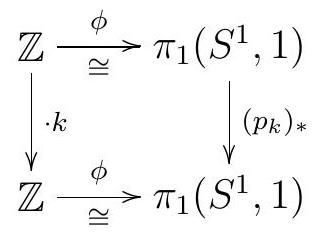
\includegraphics[max width=\textwidth]{2025_06_05_d7ed2bacd1e9ce1db1f0g-014} ist $\left(p_{k} \circ \omega_{n}\right)(s)=\left(e^{2 \pi \mathrm{i} n s}\right)^{k}=e^{2 \pi \mathrm{i} k n s}=\omega_{k n}(s)$, vgl. (I.2), und daher $\left(p_{k}\right)_{*}(\phi(n))=\left(p_{k}\right)_{*}\left(\left[\omega_{n}\right]\right)=\left[p_{k} \circ \omega_{n}\right]=\left[\omega_{k n}\right]=\phi(k n)$. Beachte, dass $p_{1}$ und $p_{-1}$ beides Homöomorphismen sind, die induzierten Homomorphismen $\left(p_{1}\right)_{*}$ und $\left(p_{-1}\right)_{*}$ aber nicht übereinstimmen.

Für den Beweis von Satz I.2.1 betrachten wir die Abbildung

$$
p: \mathbb{R} \rightarrow S^{1}, \quad p(s):=e^{2 \pi \mathbf{i} s}
$$

Drei Eigenschaften von $p$ werden wesentlich in den Beweis von Satz I.2.1 eingehen. Erstens ist der Definitionsbereich $\mathbb{R}$ einfach zusammenhängend, siehe Beispiel I.1.23, weiters ist $p^{-1}(1)=\mathbb{Z} \subseteq \mathbb{R}$ und schließlich hat $p$ die sogenannte Homotopieliftungseigenschaft.\\
I.2.3. Proposition (Homotopieliftungseigenschaft). Es seien $H: Y \times I \rightarrow S^{1}$ und $\tilde{h}: Y \rightarrow \mathbb{R}$ stetig mit $p \circ \tilde{h}=H_{0}$. Dann existiert genau eine stetige Abbildung $\tilde{H}: Y \times I \rightarrow \mathbb{R}$ mit $p \circ \tilde{H}=H$ und $\tilde{H}_{0}=\tilde{h}$. ${ }^{4}$\\
I.2.4. Bemerkung. Bezeichnen wir mit $\iota_{0}: Y \rightarrow Y \times I, \iota_{0}(y):=(y, 0)$, die Inklusion bei 0, so lässt sich die Aussage von Proposition I.2.3 schön an nebenstehenden Diagramm veranschaulichen. Die Voraussetzung in Proposition I.2.3 besagt gerade, dass das äußere Quadrat kommutiert, dh. die Komposition $p \circ \tilde{h}$ stimmt mit der Komposition $H \circ \iota_{0}$ überein. Die Konklusion von Proposition I.2.3 besagt nun, dass eine eindeutige stetige Abbildung\\
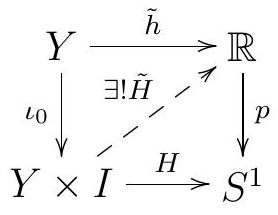
\includegraphics[max width=\textwidth]{2025_06_05_d7ed2bacd1e9ce1db1f0g-015} $\tilde{H}: Y \times I \rightarrow \mathbb{R}$ existiert, die die beiden Dreiecke kommutativ macht, dh. die Komposition $\tilde{H} \circ \iota_{0}$ stimmt mit $\tilde{h}$ überein, und $p \circ \tilde{H}$ stimmt mit $H$ überein.\\
I.2.5. Bemerkung. Sind $f: X \rightarrow S^{1}$ und $\tilde{f}: X \rightarrow \mathbb{R}$ stetige Abbildungen mit $p \circ \tilde{f}=f$, dann wird $\tilde{f}$ ein Lift von $f$ genannt. In diesem Fall sagen wir auch $f$ kann über $p$ zu einer stetigen Abbildung $\tilde{f}$ geliftet werden. Nicht jede Abbildung lässt sich stetige über $p$ liften, etwa besitzt die identische Abbildung $\operatorname{id}_{S^{1}}: S^{1} \rightarrow S^{1}$ keinen stetigen Lift, siehe Satz I.2.1. Existiert ein Lift $\tilde{f}$ von $f$, dann ist dieser nicht eindeutig, denn durch Translation mit ganzen Zahlen erhalten wir unendlich viele weitere Lifte.

Wir verschieben den Beweis von Proposition I.2.3 und betrachten zunächst die folgenden beiden Spezialfälle: $Y=\{*\}$, der einpunktige Raum, sowie $Y=I$, siehe die Propositionen I.2.6 und I.2.8 unten.\\
I.2.6. Proposition. Es sei $f: I \rightarrow S^{1}$ ein Weg und $\tilde{x} \in \mathbb{R}$ mit $p(\tilde{x})=f(0)$. Dann existiert genau ein Weg $\tilde{f}: I \rightarrow \mathbb{R}$ mit $p \circ \tilde{f}=f$ und $\tilde{f}(0)=\tilde{x}$.

Beweis. Wenden wir Proposition I.2.3 auf den einpunktigen Raum $Y:=\{*\}$, die Abbildung $\tilde{h}:\{*\} \rightarrow \mathbb{R}, \tilde{h}(*):=\tilde{x}$, und $H:\{*\} \times I \rightarrow S^{1}, H(*, t):=f(t)$, an so erhalten wir eine eindeutige stetige Abbildung $\tilde{H}:\{*\} \times I \rightarrow \mathbb{R}$ die $p \circ \tilde{H}=H$ und $\tilde{H}_{0}=\tilde{h}$ erfüllt. Offensichtlich hat dann $\tilde{f}(t):=\tilde{H}(*, t)$ alle gewünschten Eigenschaften.\\
I.2.7. Beispiel. Für die Wege $\tilde{\omega}_{n}: I \rightarrow \mathbb{R}, \tilde{\omega}_{n}(s):=n s, n \in \mathbb{Z}$, gilt $\tilde{\omega}_{n}(0)=0$, $\tilde{\omega}_{n}(1)=n$ und $p \circ \tilde{\omega}_{n}=\omega_{n}$. Insbesondere ist $\tilde{\omega}_{n}$ ein Lift von $\omega_{n}$, siehe (I.2).

\footnotetext{${ }^{4}$ Ist $G: Y \times I \rightarrow X$ eine Abbildung und $t \in I$ so schreiben wir $G_{t}: Y \rightarrow X$ für die durch $G_{t}(y):=G(y, t)$ definierte Abbildung. In dieser Proposition also $H_{0}(y):=H(y, 0)$ und $\tilde{H}_{0}(y):=\tilde{H}(y, 0)$.
}Beachte, dass $\tilde{\omega}_{n}$ nur für $n=0$ geschlossen ist. Wir werden die Wege $\tilde{\omega}_{n}$ auch im Beweis von Satz I.2.1 unten verwenden.\\
I.2.8. Proposition. Es sei $\tilde{h}: I \rightarrow \mathbb{R}$ ein Weg und $H: I \times I \rightarrow S^{1}$ eine Homotopie von Wegen mit $H_{0}=p \circ \tilde{h}$. Dann existiert eine eindeutige Homotopie von Wegen $\tilde{H}: I \times I \rightarrow \mathbb{R}$ mit $p \circ \tilde{H}=H$ und $\tilde{H}_{0}=\tilde{h}$.

Beweis. Wenden wir Proposition I.2.3 mit $Y:=I$ an, so erhalten wir eine eindeutige stetige Abbildung $\tilde{H}: I \times I \rightarrow \mathbb{R}$ mit $p \circ \tilde{H}=H$ und $\tilde{H}_{0}=\tilde{h}$. Es ist noch zu zeigen, dass $\tilde{H}$ eine Homotopie relativ Endpunkten ist. Für $i=0,1$ betrachten wir dazu den Weg $\tilde{\sigma}_{i}: I \rightarrow \mathbb{R}, \tilde{\sigma}_{i}(t):=\tilde{H}(i, t)$. Aus $p \circ \tilde{H}=H$ folgt $\left(p \circ \tilde{\sigma}_{i}\right)(t)=H(i, t)$ und dies ist konstant in $t$, da $H$ eine Homotopie von Wegen ist. Aus $\tilde{H}_{0}=\tilde{h}$ erhalten wir weiters $\tilde{\sigma}_{i}(0)=\tilde{H}(i, 0)=\tilde{h}(i)$. Aus der Eindeutigkeitsaussage in Proposition I.2.6 folgt daher, dass $\tilde{\sigma}_{i}$ mit dem konstanten Weg $c_{\tilde{h}(i)}$ übereinstimmen muss. Also ist $\tilde{H}$ tatsächlich eine Homotopie von Wegen.

Beweis von Satz I.2.1. Zur Surjektivität von $\phi$ : Sei $f: I \rightarrow S^{1}$ eine Schleife bei $1 \in S^{1}$. Zu zeigen ist, dass $n \in \mathbb{Z}$ mit $\phi(n)=[f]$ existiert. Nach Proposition I.2.6, und da $p(0)=1$, existiert ein Weg $\tilde{f}: I \rightarrow \mathbb{R}$ mit $p \circ \tilde{f}=f$ und $\tilde{f}(0)=0$. Da $p(\tilde{f}(1))=f(1)=1$, und weil $p^{-1}(1)=\mathbb{Z}$, muss $\tilde{f}(1)$ ganzzahlig sein, $n:=\tilde{f}(1) \in \mathbb{Z}$. Beobachte nun, dass $\tilde{f}$ und $\tilde{\omega}_{n}$ aus Beispiel I.2.7 beides Wege in $\mathbb{R}$ sind die bei 0 starten und bei $n$ enden. Aus dem einfachen Zusammenhang von $\mathbb{R}$, siehe Beispiel I.1.23, und Proposition I.1.21 erhalten wir eine Homotopie von Wegen $\tilde{H}: I \times I \rightarrow \mathbb{R}$ von $\tilde{H}_{0}=\tilde{\omega}_{n}$ nach $\tilde{H}_{1}=\tilde{f}$. Es ist dann $H:=p \circ \tilde{H}: I \times I \rightarrow S^{1}$ eine Homotopie von Wegen von $H_{0}=p \circ \tilde{H}_{0}=p \circ \tilde{\omega}_{n}=\omega_{n}$ nach $H_{1}=p \circ \tilde{H}_{1}=p \circ \tilde{f}=f$. Daher gilt $\phi(n)=\left[\omega_{n}\right]=[f]$.

Zur Injektivität von $\phi$ : Seien also $m, n \in \mathbb{Z}$ und $\phi(m)=\phi(n)$. Zu zeigen ist $n=m$. Da $\phi(m)=\phi(n)$ existiert eine Homotopie von Wegen $H: I \times I \rightarrow S^{1}$ von $H_{0}=\omega_{m}$ nach $H_{1}=\omega_{n}$. Nach Proposition I.2.8, und da $p \circ \tilde{\omega}_{m}=\omega_{m}$, existiert eine Homotopie von Wegen $\tilde{H}: I \times I \rightarrow \mathbb{R}$ mit $p \circ \tilde{H}=H$ und $\tilde{H}_{0}=\tilde{\omega}_{m}$. Da $\tilde{H}$ die Endpunkte fixiert gilt insbesondere $\tilde{H}_{1}(0)=\tilde{H}_{0}(0)=\tilde{\omega}_{m}(0)=0$ und $\tilde{H}_{1}(1)=\tilde{H}_{0}(1)=\tilde{\omega}_{m}(1)=m$. Weiters ist $p \circ \tilde{H}_{1}=H_{1}=\omega_{n}$. Aus der Eindeutigkeitsaussage in Proposition I.2.6 folgt daher $\tilde{H}_{1}=\tilde{\omega}_{n}$, und wir erhalten $m=\tilde{H}_{1}(1)=\tilde{\omega}_{n}(1)=n$.

Zur Homomorphismus Eigenschaft von $\phi$ : Seien $m, n \in \mathbb{Z}$. Es ist zu zeigen $\phi(m+n)=\phi(m) \phi(n)$. Betrachte dazu die Translation $\tau_{m}: \mathbb{R} \rightarrow \mathbb{R}, \tau_{m}(s):=m+s$. Dann ist $\tilde{\omega}_{m}\left(\tau_{m} \circ \tilde{\omega}_{n}\right)$ ein Weg in $\mathbb{R}$ der bei 0 startet und bei $m+n$ endet. Auch $\tilde{\omega}_{m+n}$ ist ein Weg von 0 nach $m+n$. Da $\mathbb{R}$ einfach zusammenhängend ist, existiert eine Homotopie von Wegen $\tilde{H}: I \times I \rightarrow \mathbb{R}$ von $\tilde{H}_{0}=\tilde{\omega}_{m+n} \operatorname{nach} \tilde{H}_{1}=\tilde{\omega}_{m}\left(\tau_{m} \circ \tilde{\omega}_{n}\right)$, siehe Proposition I.1.21. Es ist daher $H:=p \circ \tilde{H}: I \times I \rightarrow S^{1}$ eine Homotopie von Wegen von $H_{0}=p \circ \tilde{H}_{0}=p \circ \tilde{\omega}_{m+n}=\omega_{m+n}$ nach $H_{1}=p \circ \tilde{H}_{1}=p \circ\left(\tilde{\omega}_{m}\left(\tau_{m} \circ \tilde{\omega}_{n}\right)\right)=$ $\left(p \circ \tilde{\omega}_{m}\right)\left(p \circ \tau_{m} \circ \tilde{\omega}_{n}\right)=\left(p \circ \tilde{\omega}_{m}\right)\left(p \circ \tilde{\omega}_{n}\right)=\omega_{m} \omega_{n}$. Es gilt daher $\omega_{m+n} \simeq \omega_{m} \omega_{n}$, also $\phi(m+n)=\left[\omega_{m+n}\right]=\left[\omega_{m} \omega_{n}\right]=\left[\omega_{m}\right]\left[\omega_{n}\right]=\phi(m) \phi(n)$.

Es bleibt schließlich noch Proposition I.2.3 zu beweisen. Wir beginnen mit einigen Vorbereitungen. Für den Rest des Abschnitts seien $H: Y \times I \rightarrow S^{1}$ und $\tilde{h}: Y \rightarrow \mathbb{R}$ stetig mit $p \circ \tilde{h}=H_{0}$ wie in Proposition I.2.3.\\
I.2.9. LEMMA (Überlagerungseigenschaft). Es existieren offene Teilmengen $U_{\alpha} \subseteq S^{1}$ und offene Teilmengen $\tilde{U}_{\alpha}^{j} \subseteq \mathbb{R}, \alpha \in\{0,1\}, j \in \mathbb{Z}$, mit folgenden Eigenschaften:\\
(i) $U_{0} \cup U_{1}=S^{1}$.\\
(ii) $p^{-1}\left(U_{\alpha}\right)=\bigcup_{j \in \mathbb{Z}} \tilde{U}_{\alpha}^{j}$.\\
(iii) $\tilde{U}_{\alpha}^{j} \cap \tilde{U}_{\alpha}^{k}=\emptyset$, falls $j \neq k$.\\
(iv) $\left.p\right|_{\tilde{U}_{\alpha}^{j}}: \tilde{U}_{\alpha}^{j} \rightarrow U_{\alpha}$ ist ein Homöomorphismus.

Beweis. Setzen wir $U_{0}:=S^{1} \backslash\{1\}$ und $U_{1}:=S^{1} \backslash\{-1\}$, so ist $\left\{U_{0}, U_{1}\right\}$ eine offene Überdeckung von $S^{1}$, und es gilt $p^{-1}\left(U_{0}\right)=\mathbb{R} \backslash \mathbb{Z}$ sowie $p^{-1}\left(U_{1}\right)=$ $\mathbb{R} \backslash\left(\frac{1}{2}+\mathbb{Z}\right)$. Die Intervalle $\tilde{U}_{0}^{j}:=(j, j+1)$ und $\tilde{U}_{1}^{j}:=\left(j-\frac{1}{2}, j+\frac{1}{2}\right), j \in \mathbb{Z}$, haben dann die gewünschten Eigenschaften.\\
I.2.10. Lemma. Zu jedem Punkt $y \in Y$ existieren eine offene Umgebung $N$ von $y, 0=t_{0}<t_{1}<t_{2}<\cdots<t_{n}=1$ und $\alpha_{1}, \ldots, \alpha_{n} \in\{0,1\}$, sodass für jedes $i=1, \ldots, n$ gilt $H\left(N \times\left[t_{i-1}, t_{i}\right]\right) \subseteq U_{\alpha_{i}}$.

Beweis. Sei also $y \in Y$ fix. Zu jedem $s \in I$ existiert $\alpha_{s} \in\{0,1\}$ mit $H(y, s) \in$ $U_{\alpha_{s}}$, siehe Lemma I.2.9(i). Da $H$ stetig ist, finden wir zu jedem $s \in I$ eine offene Umgebung $N_{s}$ von $y$ und eine offene Umgebung $J_{s}$ von $s$ mit $H\left(N_{s} \times J_{s}\right) \subseteq U_{\alpha_{s}}$. Klarerweise bildet $\left\{J_{s}\right\}_{s \in I}$ eine offene Überdeckung von $I$. Da $I$ kompakt ist, existieren $0=t_{0}<t_{1}<\cdots<t_{n}=1$ und $s_{1}, \ldots, s_{n} \in I$ mit $\left[t_{i-1}, t_{i}\right] \subseteq J_{s_{i}}$, $1 \leq i \leq n$, siehe Lemma I.1.28. Betrachte nun die offene Umgebung $N:=\bigcap_{i=1}^{n} N_{s_{i}}$ von $y$. Für $1 \leq i \leq n$ gilt dann $H\left(N \times\left[t_{i-1}, t_{i}\right]\right) \subseteq H\left(N_{s_{i}} \times J_{s_{i}}\right) \subseteq U_{\alpha_{s_{i}}}$. Mit $\alpha_{i}:=\alpha_{s_{i}}$ folgt daher die Behauptung.\\
I.2.11. Lemma. Zu jedem $y \in Y$ existieren eine offene Umgebung $V$ von $y$ und eine stetige Abbildung $\tilde{G}: V \times I \rightarrow \mathbb{R}$ mit $p \circ \tilde{G}=\left.H\right|_{V \times I}$ und $\tilde{G}_{0}=\left.\tilde{h}\right|_{V}$.

Beweis. Sei also $y \in Y$ fix. Nach Lemma I.2.10 existieren eine offene Umgebung $N$ von $y, 0=t_{0}<t_{1}<\cdots<t_{n}=1$ und $\alpha_{1}, \ldots, \alpha_{n} \in\{0,1\}$, sodass

$$
H\left(N \times\left[t_{i-1}, t_{i}\right]\right) \subseteq U_{\alpha_{i}} \quad \text { für } i=1,2, \ldots, n .
$$

Wegen (I.4) und $p \circ \tilde{h}=H_{0}$ ist $p(\tilde{h}(y))=H_{t_{0}}(y) \in U_{\alpha_{1}}$, also existiert $j_{1} \in \mathbb{Z}$ mit $\tilde{h}(y) \in \tilde{U}_{\alpha_{1}}^{j_{1}}$, siehe Lemma I.2.9(ii). Betrachte die offene Umgebung $V^{1}:=$ $N \cap \tilde{h}^{-1}\left(\tilde{U}_{\alpha_{1}}^{j_{1}}\right)$ von $y$ und die Abbildung

$$
\tilde{G}^{1}: V^{1} \times\left[t_{0}, t_{1}\right] \rightarrow \tilde{U}_{\alpha_{1}}^{j_{1}} \subseteq \mathbb{R}, \quad \tilde{G}^{1}:=\left.\left(\left.p\right|_{\tilde{U}_{\alpha_{1}}^{j_{1}}}\right)^{-1} \circ H\right|_{V^{1} \times\left[t_{0}, t_{1}\right]}
$$

Nach (I.4) und Lemma I.2.9(iv) ist $\tilde{G}^{1}$ wohldefiniert und stetig. Offensichtlich gilt $p \circ \tilde{G}^{1}=\left.H\right|_{V^{1} \times\left[t_{0}, t_{1}\right]}$. Aus $H_{0}=p \circ \tilde{h}$ erhalten wir $p \circ \tilde{G}_{t_{0}}^{1}=\left.H_{t_{0}}\right|_{V^{1}}=\left.p \circ \tilde{h}\right|_{V^{1}}$, und da $p$ auf $\tilde{U}_{\alpha_{1}}^{j_{1}}$ injektiv ist folgt $\tilde{G}_{t_{0}}^{1}=\left.\tilde{h}\right|_{V^{1}}$.

Wegen (I.4) und $p \circ \tilde{G}^{1}=\left.H\right|_{V^{1} \times\left[t_{0}, t_{1}\right]}$ ist $p\left(\tilde{G}_{t_{1}}(y)\right)=H_{t_{1}}(y) \in U_{\alpha_{2}}$, also existiert $j_{2} \in \mathbb{Z}$ mit $\tilde{G}_{t_{1}}^{1}(y) \in \tilde{U}_{\alpha_{2}}^{j_{2}}$, siehe Lemma I.2.9(ii). Betrachte die offene Umgebung $V^{2}:=V^{1} \cap\left(\tilde{G}_{t_{1}}^{1}\right)^{-1}\left(\tilde{U}_{\alpha_{2}}^{j_{2}}\right)$ von $y$ und die Abbildung

$$
\tilde{G}^{2}: V^{2} \times\left[t_{1}, t_{2}\right] \rightarrow \tilde{U}_{\alpha_{2}}^{j_{2}} \subseteq \mathbb{R}, \quad \tilde{G}^{2}:=\left.\left(\left.p\right|_{\tilde{U}_{\alpha_{2}}^{j_{2}}}\right)^{-1} \circ H\right|_{V^{2} \times\left[t_{1}, t_{2}\right]}
$$

Nach (I.4) und Lemma I.2.9(iv) ist $\tilde{G}^{2}$ wohldefiniert und stetig. Offensichtlich gilt $p \circ \tilde{G}^{2}=\left.H\right|_{V^{2} \times\left[t_{1}, t_{2}\right]}$. Es folgt $p \circ \tilde{G}_{t_{1}}^{2}=\left.H_{t_{1}}\right|_{V^{2}}=\left.p \circ \tilde{G}_{t_{1}}^{1}\right|_{V^{2}}$, und da $p$ auf $\tilde{U}_{\alpha_{2}}^{j_{2}}$ injektiv ist, erhalten wir $\tilde{G}_{t_{1}}^{2}=\left.\tilde{G}_{t_{1}}^{1}\right|_{V^{1}}$.

Induktiv fortfahrend erhalten wir offene Umgebungen $V^{1} \supseteq V^{2} \supseteq \cdots \supseteq V^{n}$ von $y$ und stetige Abbildungen $\tilde{G}^{i}: V^{i} \times\left[t_{i-1}, t_{i}\right] \rightarrow \subseteq \tilde{U}_{\alpha_{i}}^{j_{i}} \subseteq \mathbb{R}, 1 \leq i \leq n$, sodass

$$
p \circ \tilde{G}^{i}=\left.H\right|_{V^{i} \times\left[t_{i-1}, t_{i}\right]}, \quad \tilde{G}_{t_{0}}^{1}=\left.\tilde{h}\right|_{V^{1}} \quad \text { und } \quad \tilde{G}_{t_{i-1}}^{i}=\left.\tilde{G}_{t_{i-1}}^{i-1}\right|_{V^{i}} \quad \text { für } i=2, \ldots, n .
$$

Betrachte nun die offene Umgebung $V:=V^{n}$ von $y$ und definiere eine Abbildung $\tilde{G}: V \times I \rightarrow \mathbb{R}$ durch $\left.\tilde{G}\right|_{V \times\left[t_{i-1}, t_{i}\right]}:=\left.\tilde{G}^{i}\right|_{V \times\left[t_{i-1}, t_{i}\right]}$. Da $\left.\tilde{G}_{t_{i-1}}^{i}\right|_{V}=\left.\tilde{G}_{t_{i-1}}^{i-1}\right|_{V}$ ist dies wohldefiniert. Aus der Stetigkeit von $\left.\tilde{G}^{i}\right|_{V \times\left[t_{i-1}, t_{i}\right]}$ und Lemma I.1.2 folgt, dass $\tilde{G}$ stetig ist. Aus $p \circ \tilde{G}^{i}=\left.H\right|_{V^{i} \times\left[t_{i-1}, t_{i}\right]}$ erhalten wir $p \circ \tilde{G}=\left.H\right|_{V \times I}$. Schließlich folgt aus $\tilde{G}_{t_{0}}^{1}=\left.\tilde{h}\right|_{V^{1}}$ auch $\tilde{G}_{0}=\left.\tilde{h}\right|_{V}$. Also hat $\tilde{G}$ alle gewüschten Eigenschaften.\\
I.2.12. Lemma. Sind $\tilde{f}, \tilde{g}: I \rightarrow \mathbb{R}$ zwei Wege mit $p \circ \tilde{f}=p \circ \tilde{g}$ und $\tilde{f}(0)=\tilde{g}(0)$, dann gilt $\tilde{f}=\tilde{g}$.

Beweis. Wir betrachten die Menge $Z:=\{s \in I: \tilde{f}(s)=\tilde{g}(s)\}$. Da $\tilde{f}$ und $\tilde{g}$ beide stetig sind, ist $Z$ eine abgeschlossene Teilmenge von $I$. Da $\tilde{f}(0)=\tilde{g}(0)$ ist $0 \in Z$, also $Z \neq \emptyset$. Wir werden unten zeigen, dass $Z$ auch offen in $I$ ist. Aus dem Zusammenhang von $I$ folgt dann $Z=I$, also $\tilde{f}=\tilde{g}$. Um die Offenheit von $I$ zu zeigen, sei $s \in Z$. Nach Lemma I.2.9 existieren $\alpha \in\{0,1\}$ und $j \in \mathbb{Z}$ mit $\tilde{f}(s)=\tilde{g}(s) \in \tilde{U}_{\alpha}^{j}$. Betrachte die offene Umgebung $W:=\tilde{f}^{-1}\left(\tilde{U}_{\alpha}^{j}\right) \cap \tilde{g}^{-1}\left(\tilde{U}_{\alpha}^{j}\right)$ von s. Da $p \circ \tilde{f}=p \circ \tilde{g}$, und da $\left.p\right|_{\tilde{U}_{\alpha}^{j}}: \tilde{U}_{\alpha}^{j} \rightarrow U_{\alpha}$ injektiv ist, siehe Lemma I.2.9(iv), erhalten wir $\left.\tilde{f}\right|_{W}=\left.\tilde{g}\right|_{W}$. Also ist $W \subseteq Z$ und daher $Z$ offen in $I$.

Beweis von Proposition I.2.3. Nach Lemma I.2.11 existiert zu jedem $y \in$ $Y$ eine offene Umgebung $V^{y}$ von $y$ und eine stetige Abbildung $\tilde{G}^{y}: V^{y} \times I \rightarrow \mathbb{R}$ mit $p \circ \tilde{G}^{y}=\left.H\right|_{V^{y} \times I}$ und $\tilde{G}_{0}^{y}=\left.\tilde{h}\right|_{V^{y}}$. Sind $y_{1}, y_{2} \in Y$, so stimmen die Abbildungen $\tilde{G}^{y_{1}}$ und $\tilde{G}^{y_{2}}$ auf ( $V^{y_{1}} \cap V^{y_{2}}$ ) $\times I$ überein, denn ist $y \in V^{y_{1}} \cap V^{y_{2}}$ dann gilt für die Wege $\tilde{f}: I \rightarrow \mathbb{R}, \tilde{f}(t):=\tilde{G}^{y_{1}}(y, t)$, und $\tilde{g}: I \rightarrow \mathbb{R}, \tilde{g}(t):=\tilde{G}^{y_{2}}(y, t)$ sowohl $(p \circ \tilde{f})(t)=H(y, t)=(p \circ \tilde{g})(t), t \in I$, als auch $\tilde{f}(0)=\tilde{h}(y)=\tilde{g}(0)$, und daher $\tilde{G}^{y_{1}}(y, t)=\tilde{f}(t)=\tilde{g}(t)=\tilde{G}^{y_{2}}(y, t)$ für alle $t \in I$, siehe Lemma I.2.12. Wir erhalten daher eine Abbildung $\tilde{H}: Y \times I \rightarrow \mathbb{R}$, sodass $\left.\tilde{H}\right|_{V^{y} \times I}=\tilde{G}^{y}$, für jedes $y \in Y$. Da die Einschränkung von $\tilde{H}$ auf jede der offenen Mengen $V^{y} \times I$ stetig ist, muss $\tilde{H}$ stetig sein. Aus $p \circ \tilde{G}^{y}=\left.H\right|_{V^{y} \times I}$ erhalten wir $p \circ \tilde{H}=H$. Schließlich folgt aus $\tilde{G}_{0}^{y}=\left.\tilde{h}\right|_{V^{y}}$ auch $\tilde{H}_{0}=\tilde{h}$. Damit ist die Existenz der Abbildung $\tilde{H}$ in Proposition I.2.3 gezeigt. Es bleibt noch die Eindeutigkeit zu verifizieren. Seien dazu\\
$\tilde{H}^{1}, \tilde{H}^{2}: Y \times I \rightarrow \mathbb{R}$ mit $p \circ \tilde{H}^{1}=H=p \circ \tilde{H}^{2}$ und $\tilde{H}_{0}^{1}=\tilde{h}=\tilde{H}^{2}$. Zu $y \in Y$ betrachten wir die Wege $\tilde{f}: I \rightarrow \mathbb{R}, \tilde{f}(t):=\tilde{H}^{1}(y, t)$, und $\tilde{g}: I \rightarrow \mathbb{R}, \tilde{g}(t):=\tilde{H}^{2}(y, t)$. Dann gilt $(p \circ \tilde{f})(t)=H(y, t)=(p \circ \tilde{g})(t), t \in I$, sowie $\tilde{f}(0)=\tilde{h}(y)=\tilde{g}(0)$. Aus Lemma I.2.12 folgt daher $\tilde{H}^{1}(y, t)=\tilde{f}(t)=\tilde{g}(t)=\tilde{H}^{2}(y, t)$ für alle $t \in I$, also stimmen $\tilde{H}^{1}$ und $\tilde{H}^{2}$ überein.

Damit ist der Beweis von Satz I.2.1 vollständig. Im Rest dieses Abschnitts wollen wir noch einige Anwendungen besprechen.\\
I.2.13. Beispiel. Für $P \in \mathbb{R}^{n}$ ist $\varphi: S^{n-1} \times(0, \infty) \rightarrow \mathbb{R}^{n} \backslash\{P\}, \varphi(x, t):=$ $P+t x$, ein Homöomorphismus. Mit Hilfe von Satz I.1.26 und Proposition I.1.17 sehen wir, dass $\mathbb{R}^{n} \backslash\{P\}$ einfach zusammenhängend ist, falls $n \geq 3$. Im Fall $n=2$ gilt $\pi_{1}\left(\mathbb{R}^{2} \backslash\{P\}\right) \cong \mathbb{Z}$ nach Satz I.2.1 und Proposition I.1.17. Genauer, und für $P=0$, sehen wir, dass die Inklusion $\iota: S^{1} \rightarrow \mathbb{C}^{\times}:=\mathbb{C} \backslash\{0\}$ einen Isomorphismus $\iota_{*}: \pi_{1}\left(S^{1}\right) \rightarrow \pi_{1}\left(\mathbb{C}^{\times}\right)$induziert. Im Fall $n=1$ ist $\mathbb{R}^{1} \backslash\{P\}$ nicht (weg)zusammenhängend, also auch nicht einfach zusammenhängend.\\
I.2.14. SATZ. $\mathbb{R}^{2}$ ist nicht homöomorph zu $\mathbb{R}^{n}, 2 \neq n$.

Beweis. Sei also $\varphi: \mathbb{R}^{2} \xrightarrow{\cong} \mathbb{R}^{n}$ ein Homöomorphismus. Wähle einen Punkt $P \in \mathbb{R}^{2}$ und setze $Q:=\varphi(P) \in \mathbb{R}^{n}$. Die Einschränkung von $\varphi$ liefert einen Homöomorphismus $\left.\varphi\right|_{\mathbb{R}^{2} \backslash\{P\}}: \mathbb{R}^{2} \backslash\{P\} \xrightarrow{\cong} \mathbb{R}^{n} \backslash\{Q\}$. Ist $n=0$, so erhalten wir einen Widerspruch, denn $\mathbb{R}^{2} \backslash\{P\} \neq \emptyset$ aber $\mathbb{R}^{0} \backslash\{Q\}=\emptyset$. Auch im Fall $n=1$ erhalten wir einen Widerspruch, denn $\mathbb{R}^{2} \backslash\{P\}$ ist wegzusammenhängend, aber $\mathbb{R}^{1} \backslash\{Q\}$ ist nicht wegzusammenhängend. Schließlich führt auch der Fall $n>2$ auf einen Widerspruch, denn $\mathbb{R}^{2} \backslash\{P\}$ ist nicht einfach zusammenhängend, während $\mathbb{R}^{n} \backslash\{Q\}$ sehr wohl einfach zusammenhängend ist, siehe Beispiel I.2.13. Es muss daher $n=2$ sein.\\
I.2.15. Bemerkung. Es gilt allgemein $\mathbb{R}^{m} \neq \mathbb{R}^{n}$, falls $m \neq n$. Wir werden dies später zeigen, die Fundamentalgruppe reicht hierfür nicht aus. Es ist übrigens leicht zu sehen, dass $\mathbb{R}^{m}$ und $\mathbb{R}^{n}$ nur dann diffeomorph sein können, wenn $m=n$ gilt. Ist nämlich $\varphi: \mathbb{R}^{m} \rightarrow \mathbb{R}^{n}$ ein Diffeomorphismus und $x_{0} \in \mathbb{R}^{m}$ beliebig, dann folgt aus der Kettenregel, dass die Jacobimatrix $D_{x_{0}} \varphi$ einen linearen Isomorphismus zwischen $\mathbb{R}^{m}$ und $\mathbb{R}^{n}$ liefert, und dies ist natürlich nur für $m=n$ möglich.\\
I.2.16. Beispiel. Für $n \in \mathbb{N}$ bezeichnen wir mit $T^{n}:=S^{1} \times \cdots \times S^{1}$ den $n$-dimensionalen Torus. Aus Proposition I.1.17 und Satz I.2.1 folgt $\pi_{1}\left(T^{n}\right) \cong$ $\mathbb{Z}^{n}=\mathbb{Z} \times \cdots \times \mathbb{Z}$. Ein expliziter Isomorphismus ist durch $\phi_{n}: \mathbb{Z}^{n} \rightarrow \pi_{1}\left(T^{n}, x_{n}\right)$, $\phi_{n}(k):=\left[\omega_{k}\right]$, gegeben. Hierbei bezeichnet $\omega_{k}: I \rightarrow T^{n}$ den Weg $\omega_{k}(s):=$ $\left(e^{2 \pi \mathrm{i} k_{1} s}, \ldots, e^{2 \pi \mathrm{i} k_{n} s}\right), k=\left(k_{1}, \ldots, k_{n}\right) \in \mathbb{Z}^{n}$, und als Basispunkt verwenden wir $x_{n}:=(1, \ldots, 1) \in T^{n}$. Insbesondere sehen wir, dass $S^{2}$ nicht homöomorph zu $T^{2}$ sein kann, denn die Fundamentalgruppen $\pi_{1}\left(S^{2}\right)=0$ und $\pi_{1}\left(T^{2}\right) \cong \mathbb{Z}^{2}$ sind nicht isomorph, siehe Satz I.1.26 und Proposition I.1.14. Etwas allgemeiner sehen wir, dass $S^{n}$ und $T^{n}$ nicht homöomorph sind, $n \geq 2$.\\
I.2.17. Beispiel. Auf $\mathbb{R}^{n}$ betrachte die Äquivalenzrelation $x \sim y \Leftrightarrow \exists k \in$ $\mathbb{Z}^{n}: y=x+k$. Die Abbildung $p: \mathbb{R}^{n} \rightarrow T^{n}, p\left(x_{1}, \ldots, x_{n}\right):=\left(e^{2 \pi \mathbf{i} x_{1}}, \ldots, e^{2 \pi \mathbf{i} x_{n}}\right)$ induziert einen Homöomorphismus $\mathbb{R}^{n} / \sim \cong T^{n}$. Wir können den Torus daher auch als Quotient von $\mathbb{R}^{n}$ verstehen. Mit $\mathcal{M}_{m, n}(\mathbb{Z})$ bezeichnen wir die Menge aller ganzzahligen $(m \times n)$-Matrizen. Jedes $A \in \mathcal{M}_{m, n}(\mathbb{Z})$ definiert eine stetige (lineare) Abbildung $\tilde{\mu}_{A}: \mathbb{R}^{n} \rightarrow \mathbb{R}^{m}, \tilde{\mu}_{A}(x):=A x$. Beachte, dass aus $x \sim y$ auch $\tilde{\mu}_{A}(x) \sim \tilde{\mu}_{A}(y)$ folgt. Daher faktorisiert $\tilde{\mu}_{A}$ zu einer stetigen Abbildung $\mu_{A}: T^{n} \rightarrow T^{m}, p \circ \tilde{\mu}_{A}=\mu_{A} \circ p$. Beachte auch, dass $\mu_{A}$ Basispunkt erhaltend ist, $\mu_{A}:\left(T^{n}, x_{n}\right) \rightarrow\left(T^{m}, x_{m}\right)$. Wir wollen nun die induzierten Gruppenhomomorphismen $\left(\mu_{A}\right)_{*}: \pi_{1}\left(T^{n}, x_{n}\right) \rightarrow \pi_{1}\left(T^{m}, x_{m}\right)$ bestimmen. Genauer wollen wir zeigen, dass $\left(\mu_{A}\right)_{*}\left(\phi_{n}(k)\right)=$ $\phi_{m}(A k)$ gilt, $k \in \mathbb{Z}^{n}$, wobei $\phi$ den Isomorphismus aus Beispiel I.2.16 bezeichnet. In anderen Worten, wir wollen zeigen, dass das nebenstehende Diagramm kommu-\\
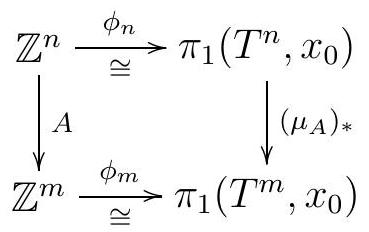
\includegraphics[max width=\textwidth]{2025_06_05_d7ed2bacd1e9ce1db1f0g-020} tiert. Für $k \in \mathbb{Z}^{n}$ betrachten wir den Weg $\tilde{\omega}_{k}: I \rightarrow \mathbb{R}^{n}$, $\tilde{\omega}_{k}(s):=s k$. Offensichtlich gilt dann $p \circ \tilde{\omega}_{k}=\omega_{k}$, wobei $\omega_{k}: I \rightarrow T^{n}$ den Weg aus Beispiel I. 2.16 bezeichnet. Weiteres haben wir die Relation $\tilde{\mu}_{A} \circ \tilde{\omega}_{k}=\tilde{\omega}_{A k}$. Wir erhalten daraus $\mu_{A} \circ \omega_{k}=\mu_{A} \circ p \circ \tilde{\omega}_{k}=p \circ \tilde{\mu}_{A} \circ \tilde{\omega}_{k}=p \circ \tilde{\omega}_{A k}=\omega_{A k}$, also $\left(\mu_{A}\right)_{*}\left(\phi_{n}(k)\right)=\left(\mu_{A}\right)_{*}\left(\left[\omega_{k}\right]\right)=\left[\mu_{A} \circ \omega_{k}\right]=\left[\omega_{A k}\right]=\phi_{m}(A k)$.

Eine Teilmenge $A$ eines topologischen Raumes $X$ heißt Retrakt von $X$, falls eine stetige Abbildung $r: X \rightarrow A$ existiert mit $r(x)=x$ für alle $x \in A$. Jede solche Abbildung $r$ wird Retraktion von $X$ auf $A$ genannt. Eine Retraktion ist also nichts anderes als eine stetige Linksinverse der kanonischen Inklusion $\iota: A \rightarrow X$, dh. $r \circ \iota=\operatorname{id}_{A}$.\\
I.2.18. Proposition. Es sei $A$ ein Retrakt von $X$, und $x_{0} \in A$. Dann ist der von der kanonischen Inklusion $\iota:\left(A, x_{0}\right) \rightarrow\left(X, x_{0}\right)$ induzierte Homomorphismus $\iota_{*}: \pi_{1}\left(A, x_{0}\right) \rightarrow \pi_{1}\left(X, x_{0}\right)$ injektiv.

Beweis. Nach Voraussetzung existiert eine Retraktion $r: X \rightarrow A$, dh. $r \circ \iota=$ $\operatorname{id}_{A}$. Insbesondere gilt $r\left(x_{0}\right)=x_{0}$, wir können daher $r$ als Abbildung punktierter Räume $r:\left(X, x_{0}\right) \rightarrow\left(A, x_{0}\right)$ auffassen. Aus Proposition I.1.13 erhalten wir $r_{*} \circ$ $\iota_{*}=(r \circ \iota)_{*}=\left(\operatorname{id}_{\left(A, x_{0}\right)}\right)_{*}=\operatorname{id}_{\pi_{1}\left(A, x_{0}\right)}$, also muss $\iota_{*}$ injektiv sein.\\
I.2.19. SATZ. $S^{1}$ ist nicht Retrakt von $D^{2}$, dh. es gibt keine stetige Abbildung $r: D^{2} \rightarrow S^{1}$ mit $r(x)=x$ für alle $x \in S^{1}$.

Beweis. Als konvexe Teilmenge von $\mathbb{R}^{2}$ ist $D^{2}$ einfach zusammenhängend, siehe Beispiel I.1.23, also $\pi_{1}\left(D^{2}\right)=0$. Nach Satz I.2.1 gilt $\pi_{1}\left(S^{1}\right) \cong \mathbb{Z}$. Es kann daher keine injektive Abbildung $\pi_{1}\left(S^{1}\right) \rightarrow \pi_{1}\left(D^{2}\right)$ existieren. Aus Proposition I.2.18 folgt nun, dass $S^{1}$ nicht Retrakt von $D^{2}$ sein kann.\\
I.2.20. Bemerkung. Die Aussage von Satz I.2.19 bleibt in beliebigen Dimensionen richtig, $S^{n-1}$ ist nicht Retrakt von $D^{n}, n \in \mathbb{N}$. Für $n=1$ ist dies trivial,\\
denn jede stetige Abbildung von $D^{1}=[-1,1]$ nach $S^{0}=\{-1,1\}$ muss konstant sein. Den Fall $n>2$ werden wir später behandeln, die Fundamentalgruppe reicht hierfür nicht aus. Wir wollen hier noch einen differentialtopologischen Beweis dieser Aussage skizzieren. Wir nehmen indirekt an es wäre $r: D^{n} \rightarrow S^{n-1}$ eine Retraktion, $r \circ \iota=\operatorname{id}_{S^{n-1}}$. Wir können $r$ durch eine glatte Retraktion approximieren, dürfen daher o.B.d.A. annehmen, dass $r$ eine glatte Abbildung ist. Nach dem Satz von Sard exisiert ein regulärer Wert $x_{0} \in S^{n-1}$. Nach dem impliziten Funktionensatz ist $M:=r^{-1}\left(x_{0}\right)$ eine kompakte glatte 1-dimensionale Teilmannigfaltigkeit von $D^{n}$ mit Rand $\partial M=M \cap S^{n-1}$. Aus $r \circ \iota=\operatorname{id}_{S^{n-1}}$ folgt $M \cap S^{n-1}=\left\{x_{0}\right\}$, also hat $M$ genau einen Randpunkt. Andererseits ist jede kompakte 1-dimensionale Mannigfaltigkeit zu einer endlichen disjunkten Vereinigung $S^{1} \sqcup \cdots \sqcup S^{1} \sqcup I \sqcup \cdots \sqcup I$ diffeomorph und muss daher eine gerade Anzahl von Randpunkten besitzen. Wir erhalten einen Widerspruch, es kann also keine solche Retraktion $r$ geben. Derselbe Beweis zeigt, dass der Rand $\partial N$ einer kompakten glatten Mannigfaltigkeit mit Rand $N$ nicht Retrakt von $N$ sein kann.\\
I.2.21. Satz (Brouwerscher Fixpunktsatz). Jede stetige Abbildung $f: D^{2} \rightarrow$ $D^{2}$ besitzt einen Fixpunkt.

Beweis. Indirekt angenommen $f: D^{2} \rightarrow D^{2}$ hätte keinen Fixpunkt. Dann können wir eine stetige Abbildung $r: D^{2} \rightarrow S^{1}$ definieren, indem wir $x \in D^{2}$ den eindeutig bestimmten Schnittpunkt des Halbstrahls $\{x+t(x-f(x)): t \geq 0\}$ mit $S^{1}$ zuordnen. Eine einfache Rechnung zeigt, dass diese Abbildung durch die Formel $r: D^{2} \rightarrow S^{1}, r(x):=x+t(x)(x-f(x))$ gegeben ist, wobei $t: D^{2} \rightarrow[0, \infty)$,

$$
t(x):=\frac{\langle x, f(x)-x\rangle+\sqrt{\langle x, f(x)-x\rangle^{2}+\left(1-|x|^{2}\right)|f(x)-x|^{2}}}{|f(x)-x|^{2}}
$$

In dieser Darstellung ist auch die Stetigkeit von $r$ evident. Für $x \in S^{1}$ gilt $r(x)=$ $x$, denn aus $1 \geq|f(x)|^{2}=|x+f(x)-x|^{2}=|x|^{2}+2\langle x, f(x)-x\rangle+|f(x)-x|^{2} \geq$ $1+2\langle x, f(x)-x\rangle+0$ folgt $\langle x, f(x)-x\rangle \leq 0$ und damit $t(x)=0$. Also ist $r$ eine Retraktion von $D^{2}$ auf $S^{1}$, ein Widerspruch zu Satz I.2.19. Daher muss $f$ einen Fixpunkt besizten.\\
I.2.22. Bemerkung. Auch Satz I.2.21 bleibt in beliebigen Dimensionen richtig, jede stetige Abbildung $f: D^{n} \rightarrow D^{n}$ besitzt einen Fixpunkt, $n \in \mathbb{N}$. Für $n=1$ folgt dies aus dem Zwischenwertsatz der Analysis. Für $n>2$ werden wir dies mit Hilfe derselben Konstruktion aus der höherdimensionalen Version von Satz I.2.19 herleiten, vgl. Bemerkung I.2.20. Es lässt sich auch umgekehrt Satz I.2.19 auf elementare Weise aus Satz I.2.21 herleiten, denn setzen wir eine Retraktion $r: D^{2} \rightarrow S^{1}$ mit der sogenannten Antipodalabbildung $A: S^{1} \rightarrow S^{1}, A(z):=-z$, zusammen, würden wir eine fixpunktfreie Abbildung $\iota \circ A \circ r: D^{2} \rightarrow D^{2}$ erhalten.\\
I.2.23. Satz (Fundamentalsatz der Algebra). Jedes nicht konstante Polynom mit komplexen Koeffizienten besitzt eine Nullstelle in $\mathbb{C}$.

Beweis. Sei also

$$
p(z)=a_{n} z^{n}+a_{n-1} z^{n-1}+\cdots+a_{1} z+a_{0}, \quad n \geq 0, a_{i} \in \mathbb{C}, a_{n} \neq 0
$$

ein Polynom und $p(z) \neq 0$ für alle $z \in \mathbb{C}$. Zu zeigen ist $n=0$. Die Schleife

$$
f: I \rightarrow S^{1}, \quad f(s):=\frac{p\left(e^{2 \pi \mathbf{i} s}\right) / p(1)}{\left|p\left(e^{2 \pi \mathbf{i} s}\right) / p(1)\right|}
$$

definiert ein Element $[f] \in \pi_{1}\left(S^{1}, 1\right)$. Die Abbildung

$$
H: I \times I \rightarrow S^{1}, \quad H(s, t):=\frac{p\left(t e^{2 \pi \mathbf{i} s}\right) / p(t)}{\left|p\left(t e^{2 \pi \mathbf{i} s}\right) / p(t)\right|}
$$

ist eine Homotopie relativ Endpunkten vom konstanten Weg $H_{0}=c_{1}$ nach $H_{1}=$ $f$. Daher repräsentiert $f$ das neutrale Element in $\pi_{1}\left(S^{1}, 1\right)$. Andererseits ist

$$
\begin{aligned}
\tilde{G}: I \times I & \rightarrow \mathbb{C}^{\times}:=\mathbb{C} \backslash\{0\} \\
\tilde{G}(s, t) & :=t^{n} p\left(e^{2 \pi \mathbf{i} s} / t\right)=a_{n} e^{2 \pi \mathbf{i} n s}+t a_{n-1} e^{2 \pi \mathbf{i}(n-1) s}+\cdots+t^{n-1} a_{1} e^{2 \pi \mathbf{i} s}+t^{n} a_{0}
\end{aligned}
$$

eine stetige Abbildung, und

$$
G: I \times I \rightarrow S^{1}, \quad G(s, t):=\frac{\tilde{G}(s, t) / \tilde{G}(0, t)}{|\tilde{G}(s, t) / \tilde{G}(0, t)|}
$$

definiert eine Homotopie relative Endpunkten von $G_{0}=w_{n}$ nach $G_{1}=f$, vgl. (I.2). Also gilt $\left[\omega_{n}\right]=[f] \in \pi_{1}\left(S^{1}, 1\right)$, und daher ist auch $\left[\omega_{n}\right]$ das neutrale Element in $\pi_{1}\left(S^{1}, 1\right)$. Aus Satz I.2.1 folgt nun $n=0$.


I.2.24. Korollar. 


Es sei $p(z)=a_{n} z^{n}+a_{n-1} z^{n-1}+\cdots+a_{1} z+a_{0}$ ein Polynom $n$-ten Grades, $n \in \mathbb{N}, a_{i} \in \mathbb{C}, a_{n} \neq 0$. Dann existieren $\alpha_{1}, \ldots, \alpha_{n} \in \mathbb{C}$, sodass

$$
p(z)=a_{n}\left(z-\alpha_{1}\right)\left(z-\alpha_{2}\right) \cdots\left(z-\alpha_{n}\right) .
$$

Über $\mathbb{C}$ zerfällt daher jedes Polynom in Linearfaktoren.\\
Beweis. Wir dürfen uns auf normierte Polynome beschränken, es sei daher o.B.d.A. $a_{n}=1$. Wir führen den Beweis durch Induktion nach $n$. Für $n=1$ ist die Aussage trivial. Für den Induktionsschritt sei nun $p$ ein normiertes Polynom $n$-ten Grades, $n \geq 2$. Nach Satz I.2.23 existiert $\alpha_{n} \in \mathbb{C}$ mit $p\left(\alpha_{n}\right)=0$. Polynomdivision mit Rest liefert ein Polynom $(n-1)$-ten Grades $q$ und eine Konstante $c \in \mathbb{C}$ mit $p(z)=q(z)\left(z-\alpha_{n}\right)+c$. Setzen wir $z=\alpha_{n}$, so erhalten wir sofort $0=$ $p\left(\alpha_{n}\right)=q\left(\alpha_{n}\right)\left(\alpha_{n}-\alpha_{n}\right)+c=c$, dh. $p(z)=q(z)\left(z-\alpha_{n}\right)$. Beachte, dass mit $p$ auch $q$ ein normiertes Polynom ist. Nach Induktionsvoraussetzung existieren daher $\alpha_{1}, \ldots, \alpha_{n-1} \in \mathbb{C}$ mit $q(z)=\left(z-\alpha_{1}\right) \cdots\left(z-\alpha_{n-1}\right)$, woraus nun $p(z)=$ $\left(z-\alpha_{1}\right) \cdots\left(z-\alpha_{n}\right)$ folgt. Damit ist der Induktionsschritt gezeigt.




\pagebreak



\subsection{Homotopieinvarianz}




\begin{DEF}{AT-H09-04-01}{Homotopie zwischen stetigen Abbildungen}
Zwei stetige Abbildungen $f, g: X \rightarrow Y$ heißen homotop falls eine stetige Abbildung $H: X \times I \rightarrow Y$ mit $H_{0}=f$ und $H_{1}=g$ existiert. Dabei bezeichnet $H_{t}: X \rightarrow Y$ die stetige Abbildung $H_{t}(x):=H(x, t)$, $t \in I$. Jede solche Abbildung $H$ wird eine Homotopie von $f$ nach $g$ genannt. Wir schreiben $f \simeq g$ oder $f \stackrel{H}{\simeq} g$. Ist $f: X \rightarrow Y$ homotop zu einer konstanten Abbildung, dh. existiert $y_{0} \in Y$ mit $f \simeq c_{y_{0}}$ wobei $c_{y_{0}}: X \rightarrow Y, c_{y_{0}}(x):=y_{0}$, dann nennen wir $f$ nullhomotop.
\end{DEF}



I.3.1. Proposition. 

\begin{PROP}{AT-H09-04-02}{Homotopie zwischen stetigen Abbildungen ist eine Äquivalenzrelation}
Homotop zu sein ist eine Äquivalenzrelation auf der Menge der stetigen Abbildungen $X \rightarrow Y$.
\end{PROP}

Beweis. 

\begin{PROOF}{AT-H09-04-03}{P: Homotopie zwischen stetigen Abbildungen ist eine Äquivalenzrelation}
Der Beweis ist völlig analog zu dem Beweis von Proposition I.1.1. Ist $f: X \rightarrow Y$ stetig, dann gilt $f \stackrel{H}{\simeq} f$ mit $H: X \times I \rightarrow Y, H(x, t):=f(x)$, also ist die Relation reflexsiv. Ist $f \stackrel{H}{\simeq} g$, dann folgt $g \stackrel{G}{\simeq} f$ mittels $G(x, t):=H(x, 1-t)$, also ist die Relation symmetrisch. Gilt $f \stackrel{H^{\prime}}{\simeq} g$ und $g \stackrel{H^{\prime \prime}}{\simeq} h$ so definiert
$$
H: X \times I \rightarrow Y, \quad H(x, t):= \begin{cases}H^{\prime}(x, 2 t) & \text { falls } 0 \leq t \leq 1 / 2 \\ H^{\prime \prime}(x, 2 t-1) & \text { falls } 1 / 2 \leq t \leq 1\end{cases}
$$
eine Homotopie von $f$ nach $h$, dh. $f \stackrel{H}{\simeq} h$, und damit ist die Relation auch transitiv. Die Stetigkeit von $H$ folgt wieder aus Lemma I.1.2.
\end{PROOF}

\begin{DEF}{AT-H09-04-04}{Homotopieklassen von stetigen Abbildungen}
Die mit obiger Äquivalenzrelation assoziierten Äquivalenzklassen werden Homotopieklassen genannt. Die Menge der Homotopieklassen stetiger Abbildungen $X \rightarrow Y$ wird mit $[X, Y]$ bezeichnet. Die von $f: X \rightarrow Y$ repräsentierte Klasse werden wir mit $[f]$ bezeichnen.
\end{DEF}



I.3.2. Beispiel. 

Bezeichnet $\{*\}$ den einpunktigen Raum, dann können wir $[\{*\}, X]$ mit der Menge der Wegzusammenhangskomponenten von $X$ identifizieren. Dabei entspricht $[f] \in[\{*\}, X]$ die (wohldefinierte) Wegzusammenhangskomponente von $X$ die $f(*)$ enthält.\\


I.3.3. Bemerkung. 

Die Menge der Homotopieklassen $\left[S^{1}, X\right]$ hängt eng mit der Fundamentalgruppe $\pi_{1}(X)$ zusammen, siehe Satz I.3.33 unten.


I.3.4. Lemma. 

\begin{LEM}{AT-H09-04-05}{Komposition erhält Homotopie von stetigen Abbildungen}
Es seien $f_{0}, f_{1}: X \rightarrow Y$ und $g_{0}, g_{1}: Y \rightarrow Z$ stetige Abbildungen mit $f_{0} \simeq f_{1}$ und $g_{0} \simeq g_{1}$. Dann gilt auch $g_{0} \circ f_{0} \simeq g_{1} \circ f_{1}$. 

Wir erhalten daher eine wohldefinierte Verknüpfung $[X, Y] \times[Y, Z] \rightarrow[X, Z]$, $([f],[g]$ ) $\mapsto[g \circ f]$.
\end{LEM}


Beweis. 

\begin{PROOF}{AT-H09-04-06}{Komposition erhält Homotopie von stetigen Abbildungen}
Es seien $F: X \times I \rightarrow Y$ und $G: Y \times I \rightarrow Z$ Homotopien mit $f_{0} \stackrel{F}{\simeq} f_{1}$ und $g_{0} \stackrel{G}{\simeq} g_{1}$. Dann liefert $H: X \times I \rightarrow Z, H(x, t):=G(F(x, t), t)$ eine Homotopie von $g_{0} \circ f_{0}$ nach $g_{1} \circ f_{1}$, dh. $g_{0} \circ f_{0} \stackrel{H}{\simeq} g_{1} \circ f_{1}$.
\end{PROOF}



I.3.5. Definition (Homotopieäquivalenz). 


\begin{DEF}{AT-H09-04-07}{Homotopieäquivalenz zwischen topologischen Räumen}
Eine stetige Abbildung $f: X \rightarrow$ $Y$ wird Homotopieäquivalenz genannt, falls eine stetige Abbildung $g: Y \rightarrow X$ existiert, sodass $g \circ f \simeq \operatorname{id}_{X}$ und $f \circ g \simeq \operatorname{id}_{Y}$ gilt. 

Zwei topologische Räume $X$ und $Y$ heißen homotopieäquivalent, falls eine Homotopieäquivalenz $f: X \rightarrow Y$ existiert. In diesem Fall schreiben wir $X \simeq Y$, und sagen auch $X$ und $Y$ haben denselben Homotopietyp.
\end{DEF}



\begin{REM}{AT-H09-04-08}{Eigenschaften der Homotopieäquivalenz}
Jeder Homöomorphismus $f: X \rightarrow Y$ ist eine Homotopieäquivalenz, denn $g:=f^{-1}: Y \rightarrow X$ erfüllt ja sogar $g \circ f=\operatorname{id}_{X}$ und $f \circ g=\operatorname{id}_{Y}$. Homöomorphe Räume sind daher stets homotopieäquivalent. 

Die identische Abbildung $\operatorname{id}_{X}$ : $X \rightarrow X$ ist eine Homotopieäquivalenz, es gilt daher $X \simeq X$. Ist $f: X \rightarrow Y$ eine Homotopieäquivalenz und $g: Y \rightarrow X$ mit $g \circ f \simeq \operatorname{id}_{X}, f \circ g \simeq \operatorname{id}_{Y}$, dann ist trivialerweise auch $g: Y \rightarrow X$ eine Homotopieäquivalenz. 

Aus $X \simeq Y$ folgt daher $Y \simeq X$. Sind $f: X \rightarrow Y$ und $g: Y \rightarrow Z$ zwei Homotopieäquivalenzen, dann ist auch die Komposition $g \circ f: X \rightarrow Z$ eine Homotopieäquivalenz, siehe Lemma I.3.4. Aus $X \simeq Y$ und $Y \simeq Z$ folgt daher stets $X \simeq Z$. Ist $f: X \rightarrow Y$ eine Homotopieäquivalenz und ist $g: X \rightarrow X$ homotop zu $f$, dann ist auch $g$ eine Homotopieäquivalenz.
\end{REM}


I.3.6. Bemerkung. 

\begin{DEF}{AT-H09-04-09}{Stetige Abbildungen zwischen Wertebereichen induzieren Abbildungen zwischen Mengen der Homotopieklassen}
Eine stetige Abbildung $\varphi: Y_{1} \rightarrow Y_{2}$ induziert eine Abbildung 
$$\varphi_{*}:\left[X, Y_{1}\right] \rightarrow\left[X, Y_{2}\right], \varphi_{*}([f]):=[\varphi \circ f]$$ 
Nach Lemma I.3.4 ist $\varphi_{*}$ wohldefiniert.
\end{DEF}

\begin{REM}{AT-H09-04-10}{Kompositionalität der induzierten Abbildungen zwischen Mengen der Homotopieklassen}
Ist $\psi: Y_{2} \rightarrow Y_{3}$ eine weitere stetige Abbildung, dann gilt offensichtlich 
$$(\psi \circ \varphi)_{*}=\psi_{*} \circ \varphi_{*}:\left[X, Y_{1}\right] \rightarrow\left[X, Y_{3}\right]$$ 
und $\left(\operatorname{id}_{Y}\right)_{*}=\operatorname{id}_{[X, Y]}$.
\end{REM}

\begin{REM}{AT-H09-04-11}{Homotope Abbildungen zwischen Wertebereichen induzieren die gleiche Abbildungen zwischen Mengen der Homotopieklassen}
Sind $\varphi_{0}, \varphi_{1}: Y_{1} \rightarrow Y_{2}$ homotop, so gilt $$\left(\varphi_{0}\right)_{*}=\left(\varphi_{1}\right)_{*}:\left[X, Y_{1}\right] \rightarrow\left[X, Y_{2}\right]$$ 
siehe Lemma I.3.4.
\end{REM}

\begin{REM}{AT-H09-04-12}{Homotopieäquivalenzen zwischen Wertebereichen induzieren eine bijektive Abbildung zwischen Mengen der Homotopieklassen}
Ist $\varphi: Y_{1} \rightarrow Y_{2}$ eine Homotopieäquivalenz, dann induziert diese eine Bijektion $$\varphi_{*}:\left[X, Y_{1}\right] \rightarrow\left[X, Y_{2}\right]$$
Ist nämlich $\psi: Y_{2} \rightarrow Y_{1}$ mit $\psi \circ \varphi \simeq \operatorname{id}_{Y_{1}}$ und $\psi \circ \varphi \simeq \operatorname{id}_{Y_{2}}$, dann folgt 
$$\psi_{*} \circ \varphi_{*}=(\psi \circ\varphi)_{*}=\left(\operatorname{id}_{Y_{1}}\right)_{*}=\operatorname{id}_{\left[X, Y_{1}\right]}$$ 
und 
$$\varphi_{*} \circ \psi_{*}=(\varphi \circ \psi)_{*}=\left(\operatorname{id}_{Y_{2}}\right)_{*}=\operatorname{id}_{\left[X, Y_{2}\right]}$$
also ist $\psi_{*}:\left[X, Y_{2}\right] \rightarrow\left[X, Y_{1}\right]$ die Inverse von $\varphi_{*}$.
\end{REM}

\begin{REM}{AT-H09-04-13}{Homotopieäquivalenzen zwischen Wertebereichen induzieren bijektive Abbildung zwischen Mengen der Homotopieklassen der WZSH-Komponenten}
Insbesondere induziert eine Homotopieäquivalenz $\varphi: Y_{1} \rightarrow Y_{2}$ eine Bijektion zwischen der Menge der Wegzusammenhangskomponenten von $Y_{1}$ und der Menge der Wegzusammenhangskomponenten von $Y_{2}$, siehe Beispiel I.3.2.
\end{REM}


I.3.7. Bemerkung. 

\begin{REM}{AT-H09-04-14}{Analog induzieren stetige Abbildungen zwischen Definitionsbereichen Abbildungen zwischen Mengen der Homotopieklassen mit entsprechenden Definitionsbereichen}
Eine stetige Abbildung $\varphi: X_{2} \rightarrow X_{1}$ induziert eine Abbildung $\varphi^{*}:\left[X_{1}, Y\right] \rightarrow\left[X_{2}, Y\right], \varphi^{*}([f]):=[f \circ \varphi]$. Wieder ist $\varphi^{*}$ wegen Lemma I.3.4 wohldefiniert. 

Ist $\psi: X_{3} \rightarrow X_{2}$ eine weitere stetige Abbildung, dann gilt $(\varphi \circ \psi)^{*}=\psi^{*} \circ \varphi^{*}:\left[X_{1}, Y\right] \rightarrow\left[X_{3}, Y\right]$ und $\left(\operatorname{id}_{X}\right)^{*}=\operatorname{id}_{[X, Y]}$. 

Sind $\varphi_{0}, \varphi_{1}: X_{2} \rightarrow X_{1}$ homotop, so gilt $\left(\varphi_{0}\right)^{*}=\left(\varphi_{1}\right)^{*}:\left[X_{1}, Y\right] \rightarrow\left[X_{2}, Y\right]$, siehe Lemma I.3.4. 

Ist $\varphi: X_{2} \rightarrow X_{1}$ eine Homotopieäquivalenz, dann induziert diese eine Bijektion $\varphi^{*}:\left[X_{1}, Y\right] \rightarrow\left[X_{2}, Y\right]$. Ist nämlich $\psi: X_{1} \rightarrow X_{2} \operatorname{mit} \varphi \circ \psi \simeq \operatorname{id}_{X_{1}}$ und $\psi \circ \varphi \simeq \operatorname{id}_{X_{2}}$ dann folgt $\psi^{*} \circ \varphi^{*}=(\varphi \circ \psi)^{*}=\left(\operatorname{id}_{X_{1}}\right)^{*}=\operatorname{id}_{\left[X_{1}, Y\right]}$ und $\varphi^{*} \circ \psi^{*}=(\psi \circ \varphi)^{*}=\left(\operatorname{id}_{X_{2}}\right)^{*}=\operatorname{id}_{\left[X_{2}, Y\right]}$, also ist $\psi^{*}:\left[X_{2}, Y\right] \rightarrow\left[X_{1}, Y\right]$ die Inverse von $\varphi^{*}$.
\end{REM}


I.3.8 Definition (Kontrahierbare Räume). 


\begin{DEF}{AT-H09-04-15}{Kontrahierende typologische Räume}
Ein topologischer Raum $X$ heißt kontrahierbar falls er den Homotopietyp des einpunktigen Raumes hat, $X \simeq\{*\}$.
\end{DEF}


\begin{REM}{AT-H09-04-16}{Charakterisierungen von kontrahierbaren Räume}
Ein topologischer Raum \( X \) ist genau dann \emph{kontrahierbar}, wenn eine der folgenden äquivalenten Aussagen erfüllt ist:

\begin{enumerate}[label=(\arabic*)]
\item Die konstante Abbildung
\[
c: X \rightarrow \{*\}
\]
ist eine \emph{Homotopieäquivalenz}.

\item Es existiert ein Punkt \( x_0 \in X \), sodass die Inklusionsabbildung
\[
\iota: \{x_0\} \hookrightarrow X
\]
eine \emph{Homotopieäquivalenz} ist.

\item Die identische Abbildung \( \operatorname{id}_X \) ist \emph{nullhomotop}, d.\,h.\ es existiert eine stetige Abbildung (Homotopie)
\[
H: X \times I \rightarrow X \quad \text{mit} \quad H_0 = \operatorname{id}_X \quad \text{und} \quad H_1 = c_{x_0},
\]
wobei \( c_{x_0}(x) := x_0 \) die konstante Abbildung bezeichnet.
\end{enumerate}
\end{REM}


Ein topologischer Raum $X$ ist genau dann kontrahierbar, wenn die konstante Abbildung $X \rightarrow\{*\}$ eine Homotopieäquivalenz ist. 

Dies ist genau dann der Fall, wenn $x_{0} \in X$ existiert, sodass die Inklusion $\left\{x_{0}\right\} \rightarrow X$ eine Homotopieäquivalenz ist. 

Offensichtlich ist $X$ kontrahierbar genau dann, wenn die identische Abbildung $\operatorname{id}_{X}$ nullhomotop ist, dh. wenn $x_{0} \in X$ und eine Homotopie $H: X \times I \rightarrow X$ mit $H_{0}=\operatorname{id}_{X}$ und $H_{1}=c_{x_{0}}$ existieren, wobei $c_{x_{0}}: X \rightarrow X, c_{x_{0}}(x):=x_{0}$, die konstante Abbildung bezeichnet. 


\begin{REM}{AT-H09-04-17}{Kontrahierbare Räume sind WZSH}
Ein kontrahierbarer Raum muss wegzusammenhängend sein, denn für $x \in X$ ist $t \mapsto H(x, t)$ ein Weg von $x$ nach $x_{0}$.
\end{REM} 

\begin{REM}{AT-H09-04-18}{In kontrahierbaren Räumen sind Punktinklusionen homotop zu Identitätsabbildungen des Raum}
Ist $X$ kontrahierbar und $x_{1} \in X$ beliebig, dann gilt $\operatorname{id}_{X} \simeq c_{x_{1}}$, dh. die Inklusion $\left\{x_{1}\right\} \rightarrow X$ ist eine Homotopieäquivalenz, für jedes $x_{1} \in X$. Letzteres folgt aus der Tatsache, dass ein Weg von $x_{0}$ nach $x_{1}$ als Homotopie zwischen der Inklusion $\left\{x_{0}\right\} \rightarrow X$ und der Inklusion $\left\{x_{1}\right\} \rightarrow X$ aufgefasst werden kann.
\end{REM}


I.3.9. Beispiel. 

Für einen kontrahierbaren Raum $Y$ ist jede stetige Abbildung $X \rightarrow Y$ nullhomotop, die Menge $[X, Y]$ besteht daher aus nur einem Element. Um dies einzusehen fixiere $y \in Y$. Wegen der Kontrahierbarkeit von $Y$ ist die identische Abbildung $\operatorname{id}_{Y}: Y \rightarrow Y$ homotop zur konstanten Abbildung $c_{y}$ : $Y \rightarrow Y, \operatorname{id}_{Y} \simeq c_{y}$. Sei nun $f: X \rightarrow Y$ stetig. Aus Lemma I.3.4 folgt dann $f=\operatorname{id}_{Y} \circ f \simeq c_{y} \circ f=\tilde{c}_{y}$, also ist $f$ homotop zu der konstanten Abbildung $\tilde{c}_{y}: X \rightarrow Y, \tilde{c}_{y}(x):=y$.


I.3.10. Definition (Deformationsretrakt). 

\begin{DEF}{AT-H09-04-19}{Deformationsretrakte in topologischen Räumen}
Ein Teilraum $A$ eines topologischen Raumes $X$ heißt Deformationsretrakt von $X$ falls eine Homotopie $H$ : $X \times I \rightarrow X$ mit folgenden Eigenschaften existiert:
\begin{enumerate}
\item Eine stetige Abbildung \( H: X \times I \rightarrow X \) mit
\[
H_0 = \operatorname{id}_X, \quad H_1(X) \subseteq A, \quad \text{und} \quad H_t|_A = \operatorname{id}_A \ \text{für alle } t \in I
\]
wird eine \emph{Deformation von \( X \) auf \( A \)} genannt.

\item Die Abbildung \( r := H_1: X \rightarrow A \) heißt dann \emph{Deformationsretraktion}, und \( H \) wird manchmal als \emph{retrahierende Deformation} bezeichnet.

\item Bezeichnet \( \iota: A \rightarrow X \) die kanonische Inklusion, so gilt:
\[
r \circ \iota = \operatorname{id}_A,
\]
d.\,h.\ Deformationsretraktionen sind insbesondere \emph{Retraktionen}.

\item Die Inklusion \( \iota: A \hookrightarrow X \) ist eine \emph{Homotopieäquivalenz}, da
\[
\operatorname{id}_X \simeq \iota \circ r \quad \text{(via \( H \))}.
\]

\item Es wird \emph{nicht} verlangt, dass die Homotopie \( H \) einen Punkt \( x_0 \in A \) festhält, d.\,h.\ es muss nicht gelten, dass
\[
H(x_0, t) = x_0.
\]
\end{enumerate}
\end{DEF}



I.3.11. Bemerkung. 

\begin{REM}{AT-H09-04-20}{Existenz von Einpunkt-Deformationsretrakten impliziert die Kontrahierbarkeit des Raumes}
Existiert $x_{0} \in X$, sodass der einpunktige Teilraum $\left\{x_{0}\right\} \subseteq X$ Deformationsretrakt von $X$ ist, dann ist $X$ offensichtlich kontrahierbar. Die Umkehrung stimmt i.A. jedoch nicht. Es ist nicht schwer einen kontrahierbarer Raum $X$ und ein Punkt $Q \in X$ zu konstruiert, sodass $\{Q\}$ nicht Deformationsretrakt von $X$ ist.
\end{REM}


I.3.12. Beispiel. 


Die Sphäre $S^{n-1}$ ist Deformationsretrakt von $\mathbb{R}^{n} \backslash\{0\}$, es ist nämlich $H: \mathbb{R}^{n} \backslash\{0\} \times I \rightarrow \mathbb{R}^{n} \backslash\{0\}, H(x, t):=(1-t) x+\frac{t}{|x|} x$ eine retrahierende Deformation. Insbesondere ist die kanonische Inklusion $S^{n-1} \rightarrow \mathbb{R}^{n} \backslash\{0\}$ eine Homotopieäquivalenz.




I.3.13. Beispiel (Sternförmige Teilmengen). 

Eine Teilmenge $X \subseteq \mathbb{R}^{n}$ heißt sternförmig, falls $z \in X$ mit folgender Eigenschaft existiert: $x \in X, t \in[0,1] \Rightarrow$ $t z+(1-t) x \in X$. Dies bedeutet gerade, dass die affine Strecke von $x$ nach $z$ zur Gänze in $X$ liegt. Jedes solche $z$ wird ein Zentrum von $X$ genannt. Ist $z$ ein Zentrum von $X$, dann ist $\{z\}$ ein Deformationsretrakt von $X$, eine retrahierende Deformation ist durch $H: X \times I \rightarrow X, H(x, t):=t z+(1-t) x$ gegeben. Insbesondere ist die Inklusion $\{z\} \rightarrow X$ eine Homotopieäquivalenz. Sternförmige Teilmengen sind daher stets kontrahierbar. Dasselbe gilt für konvexe Teilmengen, denn konvexe Teilmengen sind sternförmig, jeder ihrer Punkte ist Zentrum.


I.3.14. Beispiel. 

Es sei $P \in S^{n}$. Dann ist $S^{n} \backslash\{P\} \cong \mathbb{R}^{n}$ kontrahierbar, siehe Beispiel I.1.25. Jede stetige Abbildung $X \rightarrow S^{n} \backslash\{P\}$ ist daher nullhomotop, siehe Beispiel I.3.9. Insbesondere ist die Inklusion des Äquators $S^{n-1} \rightarrow S^{n}, x \mapsto(x, 0)$, nullhomotop. Hierfür lässt sich auch ganz leicht eine explizte Homotopie angeben, $H: S^{n-1} \times I \rightarrow S^{n}, H(x, t):=\left(\sqrt{1-t^{2}} x, t\right)$. Für $t=0$ erhalten wir die Inklusion des Äquators, $H_{0}(x)=(x, 0)$, und für $t=1$ erhalten wir die konstante Abbildung $H_{1}(x)=(0, \ldots, 0,1)$.\\


I.3.15. Beispiel. 

Ist $A$ Deformationsretrakt von $X$, und ist $B$ Deformationsretrakt von $Y$, dann ist $A \times B$ Deformationsretrakt von $X \times Y$. Sind nämlich $G: X \times I \rightarrow X$ und $H: Y \times I \rightarrow Y$ retrahierende Deformationen von $X$ auf $A$ bzw. von $Y$ auf $B$, so ist $(x, y, t) \mapsto(G(x, t), H(y, t))$ eine retrahierende Deformation von $X \times Y$ auf $A \times B$.

Für die Konstruktion von Homotopien auf Quotientenräumen wird sich folgendes Resultat der mengentheoretischen Topologie als hilfreich erweisen, ein Beweis findet sich in [14, I.7.9 Satz 5].

I.3.16. Lemma. 

Es sei $\backslash~\{\}$ eine Äquivalenzrelation auf einem topologischen Raum $X$, und es bezeichne $p: X \rightarrow X / \sim$ die kanonische Projektion auf den Quotientenraum. Weiters sei $K$ ein lokalkompakter Hausdorffraum. Dann ist
$$
p \times \operatorname{id}_{K}: X \times K \rightarrow(X / \sim) \times K
$$
eine Quotientenabbildung, dh. eine Teilmenge $U \subseteq(X / \sim) \times K$ ist genau dann offen, wenn $\left(p \times \mathrm{id}_{K}\right)^{-1}(U)$ offen in $X \times K$ ist.


I.3.17. Lemma. 

Es sei $\sim$ eine Äquivalenzrelation auf einem topologischen Raum $X$, und es bezeichne $p: X \rightarrow X / \sim$ die Projektion auf den Quotientenraum. Weiters sei $\tilde{H}: X \times I \rightarrow Y$ eine Homotopie mit folgender Eigenschaft
$$
x_{1}, x_{2} \in X, t \in I, x_{1} \sim x_{2} \Rightarrow \tilde{H}\left(x_{1}, t\right)=\tilde{H}\left(x_{2}, t\right)
$$
Dann existiert genau eine Homotopie $H:(X / \sim) \times I \rightarrow Y$ mit $H(p(x), t)=$ $\tilde{H}(x, t)$, für alle $x \in X$ und $t \in I$.


Beweis. 

Offensichtlich gibt es genau eine Abbildung $H:(X / \sim) \times I \rightarrow Y$ mit $H(p(x), t)=\tilde{H}(x, t)$. Es bleibt daher nur die Stetigkeit von $H$ zu zeigen. Dies folgt aber sofort aus Lemma I.3.16 und der Stetigkeit von $\tilde{H}$.



Ist $A$ ein nichtleerer Teilraum eines topologischen Raumes $X$, dann schreiben wir $X / A$ für den Raum der aus $X$ entsteht wenn wir $A$ zu einem einzigen Punkt kollabieren. Genauer bezeichnet $\sim$ die von $a \sim b, a, b \in A$, erzeugte Äquivalenzrelation auf $X$, dann definieren wir $X / A:=X / \sim$ und versehen $X / A$ mit der Quotiententopologie. Wir erhalten eine stetige Abbildung $p: X \rightarrow X / A$, die als kanonische Projektion bezeichnet wird. Sie bildet ganz $A$ auf einen einzigen Punkt in $X / A$ ab den wir mit $*:=p(A)$ bezeichnen. Wir können den Quotienten daher auch als punktierten Raum ( $X / A, *$ ) auffassen. Ist ( $Z, z_{0}$ ) ein punktierter Raum und $f: X \rightarrow Z$ eine stetige Abbildung mit $f(A)=\left\{z_{0}\right\}$, dann gibt es genau eine Abbildung punktierter Räume $\bar{f}:(X / A, *) \rightarrow\left(Z, z_{0}\right)$, sodass $\bar{f} \circ p=f$. Die Stetigkeit von $\bar{f}$ folgt sofort aus der Definition der Quotiententopologie auf $X / A$.\\


I.3.18. Beispiel (Kegel). 


Ist $X$ ein topologischer Raum, dann wird
$$
C X:=(X \times I) /(X \times\{0\})
$$
der Kegel über $X$ genannt. Der Basispunkt $\{*\}$ ist ein Deformationsretrakt von $C X$, die Abbildung $\tilde{H}:(X \times I) \times I \rightarrow X \times I, \tilde{H}(x, s, t):=(x,(1-t) s)$, faktorisiert zu einer retrahierenden Deformation $H: C X \times I \rightarrow C X$ auf den Punkt $\{*\}$. Die Stetigkeit von $H$ folgt aus Lemma I.3.17. Insbesondere ist die kanonische Inklusion $\{*\} \rightarrow C X$ eine Homotopieäquivalenz, und $C X$ daher kontrahierbar. Die Abbildung $\iota: X \rightarrow C X, \iota(x):=[(x, 1)]$, ist ein Homöomorphismus auf ihr Bild, wir können $X$ daher als Teilraum von $C X$ auffassen. Offensichtlich ist $C X \backslash\{*\}$ eine offene Umgebung von $\iota(X)$, und $\iota(X)$ ist Deformationsretrakt dieser Umgebung, denn $C X \backslash\{*\} \cong X \times(0,1]$.

Ist $A \subseteq Y$ und $\varphi: A \rightarrow X$ stetig, dann definieren wir

$$
X \cup_{\varphi} Y:=(X \sqcup Y) / \sim
$$

wobei $\sim$ die von $a \sim \varphi(a), a \in A$, erzeugte Äquivalenzrelation auf der disjunkten Vereinigung $X \sqcup Y$ bezeichnet. Wir sagen der Raum $X \cup_{\varphi} Y$ entsteht aus $X$ durch Ankleben von $Y$ längs $\varphi$. Wir erhalten zwei kanonische stetige Abbildungen $\iota_{X}$ : $X \rightarrow X \cup_{\varphi} Y$ und $\hat{\varphi}: Y \rightarrow X \cup_{\varphi} Y$. Die Abbildung $\iota_{X}$ ist ein Homöomorphismus auf ihr Bild, wir können $X$ daher als Teilraum von $X \cup_{\varphi} Y$ auffassen. Bezeichnet $\iota_{A}: A \rightarrow Y$ die kanonsische Inklusion, dann gilt offensichtlich $\iota_{X} \circ \varphi=\hat{\varphi} \circ \iota_{A}$.\\
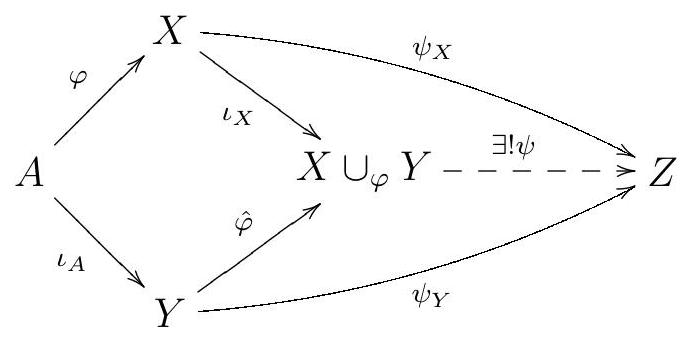
\includegraphics[max width=\textwidth]{2025_06_05_d7ed2bacd1e9ce1db1f0g-027} Der verklebte Raum $X \cup_{\varphi} Y$ hat folgende universelle Eigenschaft. Sind $\psi_{X}: X \rightarrow$ $Z$ und $\psi_{Y}: Y \rightarrow Z$ zwei stetige Abbildungen mit $\psi_{X} \circ \varphi=\psi_{Y} \circ \iota_{A}$ dann existiert eine eindeutige stetige Abbildung $\psi: X \cup_{\varphi} Y \rightarrow Z$ mit $\psi_{X}=\psi \circ \iota_{X}$ und $\psi_{Y}=\psi \circ \hat{\varphi}$. Wir werden diese Abbildung mit $\psi_{X} \cup_{\varphi} \psi_{Y}:=\psi$ bezeichnen.\\




I.3.19. Lemma. 


Es sei $A$ ein Deformationsretrakt von $Y$ und $\varphi: A \rightarrow X$ stetig. Dann ist $\iota_{X}(X)$ ein Deformationsretrakt von $X \cup_{\varphi} Y$, und die kanonische Einbettung $\iota_{X}: X \rightarrow X \cup_{\varphi} Y$ daher eine Homotopieäquivalenz.

Beweis. Es sei $H: Y \times I \rightarrow Y$ eine retrahierende Deformation, dh. $H_{0}=\operatorname{id}_{Y}$, $H_{1}(Y) \subseteq A$ und $\left.H_{t}\right|_{A}=\operatorname{id}_{A}$. Betrachte die Abbildung $\tilde{G}:(X \sqcup Y) \times I \rightarrow$ $X \cup_{\varphi} Y$ die durch $\tilde{G}(x, t):=\iota_{X}(x),(x, t) \in X \times I$, und $\tilde{G}(y, t):=\hat{\varphi}(H(y, t))$, $(y, t) \in Y \times I$, definiert ist. Da $\left.H_{t}\right|_{A}=\operatorname{id}_{A}$ faktorisiert $\tilde{G}$ zu einer stetigen Abbildung $G:\left(X \cup_{\varphi} Y\right) \times I \rightarrow X \cup_{\varphi} Y$, vgl. Lemma I.3.17. Wegen $H_{0}=\operatorname{id}_{Y}$ ist $G_{0}=\operatorname{id}_{X \cup_{\varphi} Y}$. Da $H_{1}(Y) \subseteq A$ gilt $G_{1}\left(X \cup_{\varphi} Y\right) \subseteq \iota_{X}(X)$. Schließlich ist $\left.G_{t}\right|_{\iota_{X}(X)}=\operatorname{id}_{\iota_{X}(X)}$ für alle $t \in I$. Daher ist $G$ eine retrahierende Deformation und $\iota_{X}(X)$ ein Deformationsretrakt von $X \cup_{\varphi} Y$.


I.3.20. Beispiel (Abbildungszylinder). 

Es sei $\varphi: Y \rightarrow X$ stetig, und es bezeichne $\iota_{Y}: Y \rightarrow Y \times I$ die Einbettung $\iota_{Y}(y):=(y, 1)$. Wir können $\varphi$ als eine auf dem Teilraum $A:=\iota_{Y}(Y)=Y \times\{1\}$ definiert Abbildung auffassen. Der Raum $Z_{\varphi}:=$ $X \cup_{\varphi}(Y \times I)$ wird der Abbildungszylinder von $\varphi$ genannt. Wir erhalten eine kanonische Einbettung $\iota_{X}: X \rightarrow Z_{\varphi}$ und eine stetige Abbildung\\
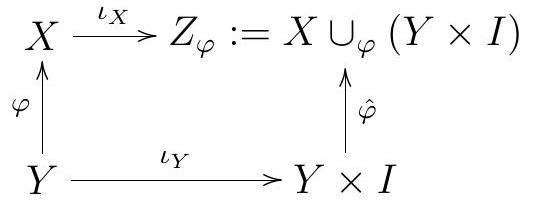
\includegraphics[max width=\textwidth]{2025_06_05_d7ed2bacd1e9ce1db1f0g-028} $\hat{\varphi}: Y \times I \rightarrow Z_{\varphi}$ mit $\iota_{X} \circ \varphi=\hat{\varphi} \circ \iota_{Y}$. Offensichtlich ist $A$ ein Deformationsretrakt von $Y \times I$, nach Lemma I.3.19 ist daher $\iota_{X}(X)$ ein Deformationsretrakt von $Z_{\varphi}$ und die Einbettung $\iota_{X}: X \rightarrow Z_{\varphi}$ eine Homotopieäquivalenz. Die Abbildung $j_{Y}: Y \rightarrow Z_{\varphi}, j_{Y}(y):=\hat{\varphi}(y, 0)$ liefert auch eine Einbettung von $Y$ in $Z_{\varphi}$. Diese ist zu $\iota_{X} \circ \varphi$ homotop, $H: Y \times I \rightarrow Z_{\varphi}$, $H(y, t):=\hat{\varphi}(y, t)$, liefert eine Homotopie von $H_{0}=j_{Y}$ nach $H_{1}=\hat{\varphi} \circ \iota_{Y}=\iota_{X} \circ \varphi$. Bis auf Homotopie(äquivalenz) können wir daher jede stetige Abbildung als Einbettung auffassen.




\begin{DEF}{AT-H09-04-21}{Homotopie relativ Basispunkt von Abbildungen punktierter Räume}
Zwei Abbildungen punktierter Räume $f, g:\left(X, x_{0}\right) \rightarrow\left(Y, y_{0}\right)$ heißen homotop relativ Basispunkt falls eine stetige Abbildung $H: I \times X \rightarrow Y$ mit $H_{0}=f$, $H_{1}=g$ und $H\left(x_{0}, t\right)=y_{0}$, für alle $t \in I$, existiert.
\end{DEF}


\begin{DEF}{AT-H09-04-22}{Setting für Homotopie relativ Basispunkt von Abbildungen punktierter Räume}
Jede solche Abbildung $H$ heißt eine Homotopie relativ Basispunkt von $f$ nach $g$. Für jedes $t \in I$ ist $H_{t}:\left(X, x_{0}\right) \rightarrow\left(Y, y_{0}\right), H_{t}(x):=H(x, t)$, eine Abbildung punktierter Räume. 

Wie in Proposition I.3.1 lässt sich zeigen, dass dies eine Äquivalenzrelation auf der Menge der Abbildungen punktierter Räume liefert. Die Äquivalenzklassen werden wir mit 
$$\left[\left(X, x_{0}\right),\left(Y, y_{0}\right)\right]$$ 
bezeichnen. 

Auch Lemma I.3.4 bleibt sinngemäß für Abbildungen punktierter Räume richtig. Eine Abbildung punktierter Räume $f:\left(X, x_{0}\right) \rightarrow\left(Y, y_{0}\right)$ wird Homotopieäquivalenz punktierter Räume genannt, falls eine Abbildung punktierter Räume $g:\left(Y, y_{0}\right) \rightarrow\left(X, x_{0}\right)$ existiert, sodass $g \circ f \simeq \operatorname{id}_{\left(X, x_{0}\right)}$ relativ Basispunkt und $f \circ g \simeq \operatorname{id}_{\left(Y, y_{0}\right)}$ relativ Basispunkt. In diesem Fall schreiben wir $\left(X, x_{0}\right) \simeq\left(Y, y_{0}\right)$. Auch die Bemerkungen I.3.6 und I.3.7 haben offensichtliche Analoga für punktierte Räume.
\end{DEF}



I.3.21. Beispiel. 

\begin{EXA}{AT-H09-04-23}{Homotopieäquivalenz punktierter Räume für Punkt-Deformationsretrakt}
Ist $A$ ein Deformationsretrakt von $X$ und $x_{0} \in A$, dann ist die kanonische Inklusion $\left(A, x_{0}\right) \rightarrow\left(X, x_{0}\right)$ eine Homotopieäquivalenz punktierter Räume.
\end{EXA}


I.3.22. Beispiel. 


\begin{EXA}{AT-H09-04-24}{Charakterisierung der Menge der WZSH-Komponenten durch  $\left[\left(S^{0}, 1\right),\left(X, x_{0}\right)\right]$}
Ist $(X, x_{0})$ ein punktierter Raum, dann können wir die Menge $\left[\left(S^{0}, 1\right),\left(X, x_{0}\right)\right]$ mit der Menge der Wegzusammenhangskomponenten von $X$ identifizieren. Dabei entspricht 
$$[f] \in\left[\left(S^{0}, 1\right),\left(X, x_{0}\right)\right]$$ 
die (eindeutig bestimmte) Wegzusammenhangskomponente von $X$ die $f(-1)$ enthält.
\end{EXA}



I.3.23. Beispiel. 


Ist $(X, x_{0})$ ein punktierter Raum, dann kann die Menge $\left[\left(S^{1}, 1\right),\left(X, x_{0}\right)\right]$ auf kanonische Art mit $\pi_{1}\left(X, x_{0}\right)$ identifiziert werden, siehe Proposition I.3.32 unten.




I.3.24. Proposition. (Homotopieinvarianz) 

\begin{PROP}{AT-H09-04-25}{Homotope Abbildungen relativ Basispunkt induzieren den gleichen Homomorphismus zwischen Fundamentalgruppen}
Sind $\varphi, \psi:\left(X, x_{0}\right) \rightarrow\left(Y, y_{0}\right)$ homotop relativ Basispunkt, dann induzieren diese denselben Homomorphismus zwischen den Fundamentalgruppen, dh. 
$$\varphi_{*}=\psi_{*}: \pi_{1}\left(X, x_{0}\right) \rightarrow \pi_{1}\left(Y, y_{0}\right)$$
\end{PROP}


Beweis. 

\begin{PROOF}{AT-H09-04-26}{P: Homotope Abbildungen relativ Basispunkt induzieren den gleichen Homomorphismus zwischen Fundamentalgruppen}
Sei $f: I \rightarrow X$ eine Schleife bei $x_{0}$. Weiters sei $H: X \times I \rightarrow Y$ eine Homotopie relativ Basispunkt von $H_{0}=\varphi$ nach $H_{1}=\psi$. Dann ist $G: I \times I \rightarrow Y$, $G(s, t):=H(f(s), t)$, eine Homotopie relativ Endpunkten von $G_{0}=H_{0} \circ f=\varphi \circ f$ nach $G_{1}=H_{1} \circ f=\psi \circ f$, also 
$$\varphi \circ f \stackrel{G}{\simeq} \psi \circ f$$ 
und damit 
$$\varphi_{*}([f])=[\varphi \circ f]=[\psi \circ f]=\psi_{*}([f])$$
\end{PROOF}



I.3.25. Proposition. 


\begin{PROP}{AT-H09-04-27}{Homotope Homöomorphismen relativ Basispunkt induzieren den gleichen Isomorphismus zwischen Fundamentalgruppen}
Ist $\varphi:\left(X, x_{0}\right) \rightarrow\left(Y, y_{0}\right)$ eine Homotopieäquivalenz punktierter Räume, dann induziert diese einen Isomorphimus zwischen den Fundamentalgruppen, $\varphi_{*}: \pi_{1}\left(X, x_{0}\right) \stackrel{\cong}{\rightarrow} \pi_{1}\left(Y, y_{0}\right)$.
\end{PROP}

Beweis. 


\begin{PROOF}{AT-H09-04-28}{P: Homotope Homöomorphismen relativ Basispunkt induzieren den gleichen Isomorphismus zwischen Fundamentalgruppen}
Sei dazu $\psi:\left(Y, y_{0}\right) \rightarrow\left(X, x_{0}\right)$, sodass $\psi \circ \varphi \simeq \operatorname{id}_{\left(X, x_{0}\right)}$ relativ Basispunkt und $\varphi \circ \psi \simeq \operatorname{id}_{\left(Y, y_{0}\right)}$ relativ Basispunkt. 

Aus Proposition I.3.24 folgt 
$$\psi_{*} \circ \varphi_{*}=(\psi \circ \varphi)_{*}=\left(\operatorname{id}_{\left(X, x_{0}\right)}\right)_{*}=\operatorname{id}_{\pi_{1}\left(X, x_{0}\right)}$$ 
sowie 
$$\varphi_{*} \circ \psi_{*}=(\varphi \circ \psi)_{*}=\left(\operatorname{id}_{\left(Y, y_{0}\right)}\right)_{*}=\operatorname{id}_{\pi_{1}\left(Y, y_{0}\right)}$$ 
Also sind $\varphi_{*}$ und $\psi_{*}$ zueinander inverse Gruppenisomorphismen.
\end{PROOF}


I.3.26. Proposition. 


\begin{PROP}{AT-H09-04-29}{Zusammenhang der induzierten Abbildungen über Homotopien und Wegtransport $\left(H_{0}\right)_{*}=\beta_{h} \circ\left(H_{1}\right)_{*}$}
Es sei $H: X \times I \rightarrow Y$ eine Homotopie, $x_{0} \in X$, $y_{0}:=H_{0}\left(x_{0}\right), y_{1}:=H_{1}\left(x_{0}\right)$, und es bezeichne $h: I \rightarrow Y$ den Wegh $(t):=H\left(x_{0}, t\right)$ von $y_{0}$ nach $y_{1}$. Dann gilt 
$$\left(H_{0}\right)_{*}=\beta_{h} \circ\left(H_{1}\right)_{*}: \pi_{1}\left(X, x_{0}\right) \rightarrow \pi_{1}\left(X, y_{0}\right)$$
\end{PROP}



Beweis. 

\begin{PROOF}{AT-H09-04-30}{P: Zusammenhang der induzierten Abbildungen über Homotopien und Wegtransport $\left(H_{0}\right)_{*}=\beta_{h} \circ\left(H_{1}\right)_{*}$}
Sei also $f: I \rightarrow X$ eine Schleife bei $x_{0}$. Die Abbildung
$$
G: I \times I \rightarrow Y, \quad G(s, t):= \begin{cases}h(4 s) & \text { falls } 0 \leq s \leq t / 4 \\ H\left(f\left(\frac{4 s-t}{4-3 t}\right), t\right) & \text { falls } t / 4 \leq s \leq 1-t / 2 \\ h(2-2 s) & \text { falls } 1-t / 2 \leq s \leq 1\end{cases}
$$
definiert eine Homotopie relativ Endpunkten in $Y$ von $G_{0}=H_{0} \circ f$ nach $G_{1}=$ $\left(h\left(H_{1} \circ f\right)\right) \bar{h}$. Also gilt 
$$\left(H_{0}\right)_{*}([f])=\left[H_{0} \circ f\right]=\left[G_{0}\right]=\left[G_{1}\right]=\left[h\left(H_{1} \circ f\right) \bar{h}\right]=\beta_{h}\left(\left[H_{1} \circ f\right]\right)=\left(\beta_{h} \circ\left(H_{1}\right)_{*}\right)([f])$$
\end{PROOF}




I.3.27. Satz (Homotopieinvarianz). 


\begin{THEO}{AT-H09-04-31}{Homotopieäquivalenz zwischen topologischen Räumen induziert Isomorphismus zwischen Fundamentalgruppen relativ Basispaaren}
Ist $\varphi: X \rightarrow Y$ eine Homotopieäquivalenz und $x_{0} \in X$, dann ist 
$$\varphi_{*}: \pi_{1}\left(X, x_{0}\right) \rightarrow \pi_{1}\left(Y, \varphi\left(x_{0}\right)\right)$$ 
ein Isomorphismus.
\end{THEO}


Beweis. 


\begin{PROOF}{AT-H09-04-32}{P: Homotopieäquivalenz zwischen topologischen Räumen induziert Isomorphismus zwischen Fundamentalgruppen relativ Basispaaren}
Da $\varphi$ eine Homtopieäquivalenz ist, existieren eine stetige Abbildung $\psi: Y \rightarrow X$ sowie Homotopien 
$H: X \times I \rightarrow X$ und $G: Y \times I \rightarrow Y$ mit $\psi \circ \varphi \stackrel{H}{\simeq} \operatorname{id}_{X}$ und $\varphi \circ \psi \stackrel{G}{\simeq} \operatorname{id}_{Y}$. 

Betrachte den Weg $h: I \rightarrow X, h(t):=H\left(x_{0}, t\right)$ von $\psi\left(\varphi\left(x_{0}\right)\right)$ nach $x_{0}$, und den Weg 
$$g: I \rightarrow Y, g(t):=G\left(\varphi\left(x_{0}\right), t\right)$$ 
von 
$$\varphi\left(\psi\left(\varphi\left(x_{0}\right)\right)\right)$$ 
nach 
$$\varphi\left(x_{0}\right)$$ 
Nach Proposition I.3.26 gilt 
$$\psi_{*} \circ \varphi_{*}=(\psi \circ \varphi)_{*}=\left(H_{0}\right)_{*}=\beta_{h} \circ\left(H_{1}\right)_{*}= \beta_{h} \circ\left(\mathrm{id}_{X}\right)_{*}=\beta_{h}$$ 
sowie 
$$\varphi_{*} \circ \psi_{*}=(\varphi \circ \psi)_{*}=\left(G_{0}\right)_{*}=\beta_{g} \circ\left(G_{1}\right)_{*}=\beta_{g} \circ\left(\mathrm{id}_{Y}\right)_{*}=\beta_{g}$$ 
Daher kommutiert das nebenstehende Diagramm:
\[
\begin{tikzcd}
\pi_1(X, x_0) \arrow[r, "\varphi_*"] \arrow[d, "\beta_h"', "\simeq"] & \pi_1(Y, \varphi(x_0)) \arrow[d, "\beta_g", "\simeq"'] \arrow[dl, "\psi_*"'] \\
\pi_1(X, \psi\varphi(x_0)) \arrow[r, "\varphi_*"'] & \pi_1(Y, \varphi\psi\varphi(x_0))
\end{tikzcd}
\]
Nach Proposition I.1.18 ist $\beta_{h}$ ein Isomorphismus, also muss $\psi_{*}$ surjektiv sein. Da $\beta_{g}$ ein Isomorphismus ist, muss $\psi_{*}$ auch injektiv sein. Damit ist $\psi_{*}$ ein Isomorphismus, woraus wir nun schließen, dass 
$$\varphi_{*}: \pi_{1}\left(X, x_{0}\right) \rightarrow \pi_{1}\left(Y, \varphi\left(x_{0}\right)\right)$$ 
ein Isomorphismus sein muss.
\end{PROOF}



I.3.28. Bemerkung. 


\begin{CONC}{AT-H09-04-36}{Fundamentalgruppe als typologische und Homotopieinvariante von WZSH Räumen}
Aus Propostion I.1.14 folgt, dass wir die Fundamentalgruppe als eine topologische Invariante wegzusammenhängender Räume auffassen können, dh. homöomorphe wegzusammenhängende topologische Räume müssen isomorphe Fundamentalgruppen haben. 

Satz I.3.27 besagt nun, dass die Fundamentalgruppe sogar eine Homotopieinvariante wegzusammenhängender Räume liefert, dh. homotopieäquivalente wegzusammenhängende topologische Räume müssen isomorphe Fundamentalgruppen haben. 

In anderen Worten, sind die Fundamentalgruppen zweier wegzusammenhängender Räume nicht isomorph, dann können die Räume nicht einmal homotopieäquivalent sein.
\end{CONC}


I.3.29. Korollar. 


\begin{KORO}{AT-H09-04-37}{Kontrahierbare Räume sind EZSH}
Kontrahierbare Räume sind einfach zusammenhängend.
\end{KORO}

Beweis. 

\begin{PROOF}{AT-H09-04-38}{P: Kontrahierbare Räume sind EZSH}
Ein kontrahierbarer Raum $X$ ist wegzusammenhägend, siehe oben, und die konstante Abbildung $X \rightarrow\{*\}$ ist eine Homotopieäquivalenz. Nach Satz I.3.27 induziert diese einen Isomorphismus $\pi_{1}(X) \cong \pi_{1}(\{*\})$. Aus $\pi_{1}(\{*\})=$ 0 folgt daher auch $\pi_{1}(X)=0$.
\end{PROOF}



I.3.30. Beispiel (Möbiusband). 

Auf $I \times[-1,1]$ betrachte die von $(0, y) \sim$ $(1,-y), y \in[-1,1]$, erzeugte Äquivalenzrelation. Der damit assoziierten Quotientenraum $M:=(I \times[-1,1]) / \sim$ wird Möbiusband genannt. Es bezeichne $p: I \times[-1,1] \rightarrow M$ die kanonische Projektion und $S:=p(I \times\{0\})$. Die retrahierende Deformation $\tilde{H}:(I \times[-1,1]) \times I \rightarrow I \times[-1,1], \tilde{H}(x, y, t):=(x,(1-t) y)$, faktorisiert zu einer retrahierenden Deformation $H: M \times I \rightarrow M, p \circ \tilde{H}_{t}=H_{t} \circ p$, von $M$ auf $S$. Daher ist $S$ ein Deformationsretrakt von $M$ und die Inklusion $S \rightarrow M$ eine Homotopieäquivalenz. Da $S$ homöomorph zu $S^{1}$ ist, erhalten wir $\pi_{1}(M) \cong \pi_{1}\left(S^{1}\right) \cong \mathbb{Z}$. Die Schleife $I \rightarrow M, s \mapsto p(s, 0)$, repräsentiert einen Erzeuger von $\pi_{1}(M)$.


I.3.31. Beispiel. 

Betrachte wieder die Abbildungen $\mu_{A}:\left(T^{n}, x_{n}\right) \rightarrow\left(T^{m}, x_{m}\right)$ aus Beispiel I.2.17, $A \in \mathcal{M}_{m, n}(\mathbb{Z})$. Aus Proposition I.3.24 und der Berechnung des induzierten Homomorphismus in Beispiel I.2.17 sehen wir, dass $\mu_{A}$ und $\mu_{B}$ nicht homotop relativ Basispunkt sind, falls $A \neq B \in \mathcal{M}_{m, n}(\mathbb{Z})$. Die Abbildung $\mathcal{M}_{m, n}(\mathbb{Z}) \rightarrow\left[\left(T^{n}, x_{n}\right),\left(T^{m}, x_{m}\right)\right], A \mapsto\left[\mu_{A}\right]$, ist daher injektiv.




\begin{DEF}{AT-H09-04-39}{Einpunktvereinigungen von punktierten Räumen}
Unter der Einpunktvereinigung zweier punktierter Räume $(X, x_{0})$ und $(Y, y_{0})$ verstehen wir den punktierten Raum der aus der disjunkten Vereinigung $X \sqcup Y$ durch Identifikation der beiden Punkte $x_{0}$ und $y_{0}$ ensteht. Genauer,
$$
\left(X, x_{0}\right) \vee\left(Y, y_{0}\right):=\left((X \sqcup Y) /\left\{x_{0}, y_{0}\right\}, *\right) .
$$
Die beiden Abbildungen punktierter Räume 
$$\iota_{X}:\left(X, x_{0}\right) \rightarrow\left(X, x_{0}\right) \vee\left(Y, y_{0}\right),\ \iota_{X}(x):=\left[\left(x, y_{0}\right)\right]$$ 
und 
$$\iota_{Y}:\left(Y, y_{0}\right) \rightarrow\left(X, x_{0}\right) \vee\left(Y, y_{0}\right),\ \iota_{Y}(y):=\left[\left(x_{0}, y\right)\right]$$ 
werden als kanonische Einbettungen bezeichnet. 

Beide sind Homöomorphismen auf ihr Bild, wir können daher ( $X, x_{0}$ ), und ebenso ( $Y, y_{0}$ ), als Teilraum von $\left(X, x_{0}\right) \vee\left(Y, y_{0}\right)$ auffassen.
\end{DEF}



Die Einpunktvereinigung hat die folgende universelle Eigenschaft. 


\begin{THEO}{AT-H09-04-40}{Universelle Eigenschaft der Einpunktvereinigung}
Sind $\varphi_{X}$ : $\left(X, x_{0}\right) \rightarrow\left(Z, z_{0}\right)$ und $\varphi_{Y}:\left(Y, y_{0}\right) \rightarrow\left(Z, z_{0}\right)$ zwei Abbildungen punktierter Räume, dann existiert eine eindeutige Abbildung punktierter Räume $\varphi:\left(X, x_{0}\right) \vee\left(Y, y_{0}\right) \rightarrow\left(Z, z_{0}\right)$, sodass $\varphi \circ \iota_{X}=\varphi_{X}$ und $\varphi \circ \iota_{Y}=\varphi_{Y}$: 
\[
\begin{tikzcd}[row sep=2em, column sep=4.5em]
(X, x_0) \arrow[dr, "\varphi_X", out=1, in=130, looseness=0.5] \arrow[d, "\iota_X"'] & \\
(X, x_0) \vee (Y, y_0) \arrow[r, "\exists ! \varphi", dashed] & (Z, z_0) \\
(Y, y_0) \arrow[u, "\iota_Y"] \arrow[ur, "\varphi_Y", out=1, in=230, looseness=0.5] &
\end{tikzcd}
\]
Diese Abbildung ist durch $\varphi\left(x, y_{0}\right):=\varphi_{X}(x)$, $x \in X$, und $\varphi\left(x_{0}, y\right):=\varphi_{Y}(y), y \in Y$, gegeben und wird mit $\varphi_{X} \vee \varphi_{Y}$ bezeichnet. Beachte, dass $\varphi_{X}\left(x_{0}\right)=z_{0}=\varphi_{Y}\left(y_{0}\right)$ und daher $\varphi_{X} \vee \varphi_{Y}$ wohldefiniert ist.
\end{THEO}


\begin{DEF}{AT-H09-04-41}{Einpunktvereinigung für beliebig viele punktierte Räume}
Analog definieren wir die Einpunktvereinigung beliebig vieler punktierter Räume $\left(X_{\alpha}, x_{\alpha}\right), \alpha \in A$, durch
$$
\bigvee_{\alpha \in A}\left(X_{\alpha}, x_{\alpha}\right):=\left(\left(\bigsqcup_{\alpha \in A} X_{\alpha}\right) /\left\{x_{\alpha}: \alpha \in A\right\}, *\right)
$$
Wieder haben wir kanonische Inklusionen $\iota_{\alpha}:\left(X_{\alpha}, x_{\alpha}\right) \rightarrow \bigvee_{\alpha^{\prime} \in A}\left(X_{\alpha^{\prime}}, x_{\alpha^{\prime}}\right)$ mit folgender universellen Eigenschaft. Ist ( $Z, z_{0}$ ) ein punktierter Raum und sind $\varphi_{\alpha}:\left(X_{\alpha}, x_{\alpha}\right) \rightarrow\left(Z, z_{0}\right)$ Abbildungen punktierter Räume, $\alpha \in A$, dann existiert genau eine Abbildung punktierter Räume $\varphi: \bigvee_{\alpha \in A}\left(X_{\alpha}, x_{\alpha}\right) \rightarrow\left(Z, z_{0}\right)$, sodass $\varphi \circ \iota_{\alpha}=\varphi_{\alpha}$ für alle $\alpha \in A$.
\end{DEF}



\begin{CONC}{AT-H09-04-42}{Einpunktvereinigung von $S^1$ als Hilfsobjekte für alternative Beschreibung der Fundamentalgruppe}
Betrachte nun wieder $S^{1} \subseteq \mathbb{C}$ mit Basispunkt $1 \in S^{1}$. Weiters bezeichnen 
$$\iota_{1}:\left(S^{1}, 1\right) \rightarrow\left(S^{1}, 1\right) \vee\left(S^{1}, 1\right)$$ 
und 
$$\iota_{2}:\left(S^{1}, 1\right) \rightarrow\left(S^{1}, 1\right) \vee\left(S^{1}, 1\right)$$ 
die beiden kanonischen Inklusionen. Definiere Abbildungen punktierter Räume:
$$
\begin{array}{ll}
\mu:\left(S^{1}, 1\right) \rightarrow\left(S^{1}, 1\right) \vee\left(S^{1}, 1\right), & \mu(z):= \begin{cases}\iota_{1}\left(z^{2}\right) & \text { falls } \operatorname{Im} z \geq 0 \\
\iota_{2}\left(z^{2}\right) & \text { falls } \operatorname{Im} z \leq 0\end{cases} \\
\nu:\left(S^{1}, 1\right) \rightarrow\left(S^{1}, 1\right), & \nu(z):=z^{-1}=\bar{z}
\end{array}
$$
\end{CONC}




Wir können damit eine alternative Beschreibung der Fundamentalgruppe geben.



I.3.32. Proposition. 


Ist $(X, x_{0})$ ein punktierter Raum, dann definiert
$$
\Psi=\Psi_{\left(X, x_{0}\right)}:\left[\left(S^{1}, 1\right),\left(X, x_{0}\right)\right] \rightarrow \pi_{1}\left(X, x_{0}\right), \quad \Psi([f]):=\left[f \circ \omega_{1}\right]
$$
eine Bijektion, siehe (I.2), und es gilt $\Psi([f]) \Psi([g])=\Psi([(f \vee g) \circ \mu])$ sowie $\Psi([f])^{-1}=\Psi([f \circ \nu])$. Diese Bijektion ist natürlich, dh. für jede Abbildung punktierter Räume $\varphi:\left(X, x_{0}\right) \rightarrow\left(Y, y_{0}\right)$ kommutiert das folgende Diagramm:
\[
\begin{tikzcd}[row sep=3.5em, column sep=4.5em]
{\left[(S^1, 1), (X, x_0)\right]} \arrow[r, "\Psi_{(X,x_0)}", "\simeq"'] \arrow[d, "\varphi_*"'] &
\pi_1(X, x_0) \arrow[d, "\varphi_*"] \\
{\left[(S^1, 1), (Y, y_0)\right]} \arrow[r, "\Psi_{(Y,y_0)}", "\simeq"'] &
\pi_1(Y, y_0)
\end{tikzcd}
\]
Dabei bezeichnet 
$$\varphi_{*}:\left[\left(S^{1}, 1\right),\left(X, x_{0}\right)\right] \rightarrow\left[\left(S^{1}, 1\right),\left(Y, y_{0}\right)\right], \varphi_{*}([f]):=[\varphi \circ f]$$


\begin{THEO}{AT-H09-04-43}{Natürliche Identifikation von $\left[\left(S^1, 1\right),\left(X, x_0\right)\right]$ mit $\pi_1\left(X, x_0\right)$}
Sei $(X, x_0)$ ein punktierter topologischer Raum. Dann gilt:
\begin{enumerate}
  \item \textbf{Definition der Abbildung:}
  \[
  \Psi = \Psi_{(X, x_0)} : \left[(S^1, 1), (X, x_0)\right] \longrightarrow \pi_1(X, x_0), \quad \Psi([f]) := [f \circ \omega_1],
  \]
  wobei $\omega_1 : I \to S^1$ die Standardparametrisierung des Einheitskreises ist.

  \item \textbf{Bijektivität:}  
  Die Abbildung $\Psi$ ist eine Bijektion (siehe z.\,B. (I.2)).

  \item \textbf{Verträglichkeit mit der Gruppenstruktur:}  
  Für alle punktierten Abbildungen $f, g : (S^1,1) \to (X,x_0)$ gilt:
  \[
  \Psi([f]) \cdot \Psi([g]) = \Psi([(f \vee g) \circ \mu]), \qquad
  \Psi([f])^{-1} = \Psi([f \circ \nu]),
  \]
  wobei $f \vee g$ die punktierte Keilsumme ist, $\mu : S^1 \to S^1 \vee S^1$ die Verklebungsabbildung der Keilsumme und $\nu : S^1 \to S^1$ die Umkehrabbildung.

  \item \textbf{Natürlichkeit:}  
  Die Abbildung $\Psi$ ist natürlich in $(X,x_0)$. Für jede Abbildung punktierter Räume
  \[
  \varphi : (X,x_0) \to (Y,y_0)
  \]
  kommutiert das folgende Diagramm:
  \[
  \begin{tikzcd}[row sep=3.5em, column sep=4.5em]
  {\left[(S^1, 1), (X, x_0)\right]} \arrow[r, "\Psi_{(X,x_0)}", "\simeq"'] \arrow[d, "\varphi_*"'] &
  \pi_1(X, x_0) \arrow[d, "\varphi_*"] \\
  {\left[(S^1, 1), (Y, y_0)\right]} \arrow[r, "\Psi_{(Y,y_0)}", "\simeq"'] &
  \pi_1(Y, y_0)
  \end{tikzcd}
  \]

  \item \textbf{Induzierter Morphismus:}  
  \[
  \varphi_* : \left[(S^1, 1), (X, x_0)\right] \longrightarrow \left[(S^1, 1), (Y, y_0)\right], \quad [f] \mapsto [\varphi \circ f].
  \]
\end{enumerate}
\end{THEO}

Beweis. 

\begin{PROOF}{AT-H09-04-44}{P: Natürliche Identifikation von $\left[\left(S^1, 1\right),\left(X, x_0\right)\right]$ mit $\pi_1\left(X, x_0\right)$}
Zunächst ist $\Psi$ wohldefiniert, denn sind $f, g:\left(S^{1}, 1\right) \rightarrow\left(X, x_{0}\right)$ homotop relativ Basispunkt, $f \stackrel{H}{\simeq} g$, dann ist $(s, t) \mapsto H\left(\omega_{1}(s), t\right)$ eine Homotopie relativ Endpunkten von $f \circ \omega_{1}$ nach $g \circ \omega_{1}$, also $\left[f \circ \omega_{1}\right]=\left[g \circ \omega_{1}\right] \in \pi_{1}\left(X, x_{0}\right)$. 

Beachte, dass $\omega_{1}: I \rightarrow S^{1}$ zu einem Homöomorphismus $I /\{0,1\} \rightarrow S^{1}$ faktorisiert. Daher definiert $f \mapsto f \circ \omega_{1}$ eine Bijektion zwischen der Menge der Abbildungen punktierter Räume $\left(S^{1}, 1\right) \rightarrow\left(X, x_{0}\right)$ und der Menge der Schleifen bei $x_{0}$. Es folgt sofort, dass $\Psi$ surjektiv ist. 

Wir sehen aber auch, dass $H \mapsto H \circ\left(\omega_{1} \times \mathrm{id}_{I}\right)$ eine Bijektion zwischen der Menge der basispunkterhaltenden Homotopien $S^{1} \times I \rightarrow X$ mit $H_{t}(1)=x_{0}$ und der Menge der Homotopien $I \times I \rightarrow X$ relativ Endpunkt $x_{0}$ liefert.Daraus folgt nun auch die Injektivität von $\Psi$

Nun zur Beschreibung der Gruppenstruktur. Für $f:\left(S^{1}, 1\right) \rightarrow\left(X, x_{0}\right)$ gilt 
$$\Psi([f])^{-1}=\left[f \circ \omega_{1}\right]^{-1}=\left[\overline{f \circ \omega_{1}}\right]=\left[f \circ \bar{\omega}_{1}\right]=\left[f \circ \nu \circ \omega_{1}\right]=\Psi([f \circ \nu])$$ 
Ist weiters $g:\left(S^{1}, 1\right) \rightarrow\left(X, x_{0}\right)$ dann gilt
$$\left((f \vee g) \circ \mu \circ \omega_{1}\right)(s)= \begin{cases}(f \vee g)\left(\iota_{1}\left(\omega_{1}(2 s)\right)\right)=f\left(\omega_{1}(2 s)\right) & \text { für } 0 \leq s \leq \frac{1}{2}, \\ (f \vee g)\left(\iota_{2}\left(\omega_{1}(2 s-1)\right)\right)=g\left(\omega_{1}(2 s-1)\right) & \text { für } \frac{1}{2} \leq s \leq 1,\end{cases}$$
wobei wir $\omega_{1}(s)^{2}=\omega_{1}(2 s)=\omega_{1}(2 s-1)$ im ersten Gleichheitszeichen verwendet haben. 

Wir schließen 
$$(f \vee g) \circ \mu \circ \omega_{1}=\left(f \circ \omega_{1}\right)\left(g \circ \omega_{1}\right)$$ 
also $\Psi([(f \vee g) \circ \mu])=$ $\Psi([f]) \Psi([g])$. 

Für die Natürlichkeitsaussage bemerken wir, 
$$\varphi_{*}\left(\Psi_{\left(X, x_{0}\right)}([f])\right)=\varphi_{*}\left(\left[f \circ \omega_{1}\right]\right)=\left[\varphi \circ\left(f \circ \omega_{1}\right)\right]=\left[(\varphi \circ f) \circ \omega_{1}\right]=\Psi_{\left(Y, y_{0}\right)}([\varphi \circ f])=\Psi_{\left(Y, y_{0}\right)}\left(\varphi_{*}([f])\right)$$
\end{PROOF}



\begin{CONC}{AT-H09-04-45}{Von Basispunkt-Homotopie zu freier Homotopie}
Für einen punktierten Raum $\left(X, x_{0}\right)$ sei 
$$\Phi_{\left(X, x_{0}\right)}: \pi_{1}\left(X, x_{0}\right) \rightarrow\left[S^{1}, X\right]$$ 
durch die Komposition
$$
\Phi_{\left(X, x_{0}\right)}: \pi_{1}\left(X, x_{0}\right) \xrightarrow{\Psi_{\left(X, x_{0}\right)}^{-1}}\left[\left(S^{1}, 1\right),\left(X, x_{0}\right)\right] \rightarrow\left[S^{1}, X\right],
$$
definiert, wobei $\Psi_{\left(X, x_{0}\right)}$ die Bijektion aus Proposition I.3.32 bezeichnet und die Abbildung $\left[\left(S^{1}, 1\right),\left(X, x_{0}\right)\right] \rightarrow\left[S^{1}, X\right]$ einer Homotopieklasse relativ Basispunkt die entsprechende sogenannte freie Homotopieklasse zuordnet.
\end{CONC}

I.3.33. Satz. 

Es sei $X$ ein wegzusammenhängender topologischer Raum und $x_0 \in X$. Die Abbildung 
$$\Phi_{\left(X, x_0\right)}: \pi_1\left(X, x_0\right) \xrightarrow{\Psi_{\left(X, x_0\right)}^{-1}}\left[\left(S^1, 1\right),\left(X, x_0\right)\right] \rightarrow\left[S^1, X\right]$$
induziert eine Bijektion zwischen der Menge der Konjugationsklassen von $\pi_1\left(X, x_0\right)$ und $\left[S^1, X\right]$. 

Für jeden Weg $h$ von $x_0=h(0)$ nach $x_1=h(1)$ gilt weiters $\Phi_{\left(X, x_1\right)}=\Phi_{\left(X, x_0\right)} \circ \beta_h$, vgl. Proposition I.1.18. 

Schließich ist $\Phi$ natürlich, dh. für jede Abbildung punktierter Räume $\varphi:\left(X, x_0\right) \rightarrow\left(Y, y_0\right)$ kommutiert das folgende Diagramm:
\[
\begin{tikzcd}
\pi_1(X, x_0) \arrow[r, "\Phi_{(X,x_0)}"] \arrow[d, "\varphi_*"'] & {[S^1, X]} \arrow[d, "\varphi_*"] \\
\pi_1(Y, y_0) \arrow[r, "\Phi_{(Y,y_0)}"'] & {[S^1, Y]}
\end{tikzcd}
\]


\begin{PROP}{AT-H09-04-46}{Bijektion zwischen Konjugationsklassen in $\pi_1\left(X, x_0\right)$ und $\left[S^1, X\right]$}
Sei \(X\) ein wegzusammenhängender topologischer Raum und \(x_0 \in X\). Dann gilt für die Abbildung
\[
\Phi_{\left(X, x_0\right)}: \pi_1\left(X, x_0\right) \xrightarrow{\Psi_{\left(X, x_0\right)}^{-1}}\left[\left(S^1, 1\right),\left(X, x_0\right)\right] \rightarrow\left[S^1, X\right],
\]
wobei die letzte Abbildung die Basispunktinformation vergisst:

\begin{enumerate}
  \item \textbf{Bijektivität auf Konjugationsklassen:} \(\Phi_{(X,x_0)}\) induziert eine Bijektion zwischen der Menge der Konjugationsklassen von \(\pi_1(X, x_0)\) und der Menge \([S^1, X]\) der freien Homotopieklassen von Schleifen in \(X\).
  
  \item \textbf{Verhalten unter Basispunktwechsel:} Für jeden Weg \(h\) von \(x_0 = h(0)\) nach \(x_1 = h(1)\) gilt
  \[
  \Phi_{(X,x_1)} = \Phi_{(X,x_0)} \circ \beta_h,
  \]
  wobei \(\beta_h: \pi_1(X, x_1) \to \pi_1(X, x_0)\) die Isomorphie durch Konjugation mit \(h\) bezeichnet (vgl. Proposition I.1.18).
  
  \item \textbf{Natürlichkeit:} Für jede Abbildung punktierter Räume \(\varphi: (X,x_0) \to (Y,y_0)\) kommutiert das folgende Diagramm:
  \[
  \begin{tikzcd}
  \pi_1(X, x_0) \arrow[r, "\Phi_{(X,x_0)}"] \arrow[d, "\varphi_*"'] & {[S^1, X]} \arrow[d, "\varphi_*"] \\
  \pi_1(Y, y_0) \arrow[r, "\Phi_{(Y,y_0)}"'] & {[S^1, Y]}
  \end{tikzcd}
  \]
\end{enumerate}
\end{PROP}


Beweis. 

\begin{PROOF}{AT-H09-04-47}{P: Bijektion zwischen Konjugationsklassen in $\pi_1\left(X, x_0\right)$ und $\left[S^1, X\right]$}
Es sei $h: I \rightarrow X$ ein Weg von $x_0:=h(0)$ nach $x_1:=h(1)$. Weiters sei $f: I \rightarrow X$ eine Schleife bei $x_1$. Dann definiert
$$
\tilde{G}: I \times I \rightarrow X, \quad \tilde{G}(s, t):= \begin{cases}h(4 s+t) & \text { falls } 0 \leq s \leq \frac{1-t}{4} \\ f\left(\frac{4 s+t-1}{3 t+1}\right) & \text { falls } \frac{1-t}{4} \leq s \leq \frac{1+t}{2} \\ h(2-2 s+t) & \text { falls } \frac{1+t}{2} \leq s \leq 1\end{cases}
$$
eine Homotopie von $\tilde{G}_0=(h f) \bar{h}$ nach $\tilde{G}_1=f$. 

Dies ist i.A. keine Homotopie relativ Endpunkten, es gilt jedoch $\tilde{G}(i, t)=h(t)$, für $i=0,1$ und alle $t \in I$. Daher faktorisiert $\tilde{G}$ zu einer Homotopie $G: S^1 \times I \rightarrow X, G\left(\omega_1(s), t\right)=H(s, t)$. Wir erhalten 
$$\Phi_{\left(X, x_1\right)}([f])=\Phi_{\left(X, x_0\right)}([h f \bar{h}]) \in\left[S^1, X\right]$$ 
und damit 
$$\Phi_{\left(X, x_1\right)}=\Phi_{\left(X, x_0\right)} \circ \beta_h$$ 
Für Wege mit $h(0)=x_0=x_1=h(1)$ besagt dies gerade, dass konjugierte Elemente in $\pi_1\left(X, x_0\right)$ auf dasselbe Element in $\left[S^1, X\right]$ abgebildet werden. 

Auch die Surjektivität von $\Phi_{\left(X, x_0\right)}$ folgt aus dieser Konstruktion. Ist nämlich $\tilde{f}: S^1 \rightarrow X$ stetig dann finden wir auf Grund des Wegzusammenhangs von $X$ einen Weg Weg $h$ von $h(0)=x_0$ nach $h(1)=f(1)$, und $G$ definiert eine Homotopie zwischen $G_1=\tilde{f}$ und der Schleife $G_0$ die wegen $G_0(1)=x_0$ im Bild der Abbildung 
$$\left[\left(S^1, 1\right),\left(X, x_0\right)\right] \rightarrow\left[S^1, X\right]$$ 
liegt. 

Es bleibt noch zu zeigen, dass $\Phi_{\left(X, x_0\right)}$ auf der Menge der Konjugationsklassen injektiv ist. Seien also $f_0, f_1: I \rightarrow X$ Schleifen bei $x_0$, sodass 
$$\Phi_{\left(X, x_0\right)}\left(\left[f_0\right]\right)=\Phi\left(\left[f_1\right]\right)$$ 
Es ist zu zeigen, dass $\left[f_0\right]$ und $\left[f_1\right]$ in $\pi_1\left(X, x_0\right)$ konjugiert sind. Nach Voraussetzung existiert eine Homotopie $H: S^1 \times I \rightarrow X$ mit $H_0 \circ \omega_1=f_0$ und $H_1 \circ \omega_1=f_1$. Betrachte nun die Schleife $h: I \rightarrow X$, $h(t):=H(1, t)$, und
$$
F: I \times I \rightarrow X, \quad F(s, t):= \begin{cases}h(4 s) & \text { falls } 0 \leq s \leq t / 4 \\ H\left(\omega_1\left(\frac{4 s-t}{4-3 t}\right), t\right) & \text { falls } t / 4 \leq s \leq 1-t / 2 \\ h(2-2 s) & \text { falls } 1-t / 2 \leq s \leq 1\end{cases}
$$
Dies ist eine Homotopie relativ Endpunkten von $F_0=H_0 \circ \omega_1=f_0$ nach 
$$F_1=\left(h\left(H_1 \circ \omega_1\right)\right) \bar{h}=\left(h f_1\right) \bar{h}$$ 
Damit ist 
$$\left[f_0\right]=\left[h f_1 \bar{h}\right]=[h]\left[f_1\right][h]^{-1}$$ 
also sind $\left[f_0\right]$ und $\left[f_1\right]$ konjugierte Elemente in $\pi_1\left(X, x_0\right)$. 

Die Natürlichkeit von $\Phi$ folgt aus der Natürlichkeitsaussage in Proposition I.3.32.
\end{PROOF}





I.3.34. Korollar (Einfacher Zusammenhang). 

\begin{KORO}{AT-H09-04-48}{Äquivalenzcharakterisierungen von Einfach Zusammenhängend}
Für einen wegzusammenhängenden topologischen Raum $X$ sind äquivalent:
\begin{enumerate}
  \item[\textup{(i)}] \(\pi_1(X) = 0\), d.\,h. \(X\) ist einfach zusammenhängend.
  \item[\textup{(ii)}] Jede stetige Abbildung \(f: S^1 \rightarrow X\) ist nullhomotop.
  \item[\textup{(iii)}] Jede stetige Abbildung \(f: S^1 \rightarrow X\) lässt sich zu einer stetigen Abbildung \(F: D^2 \rightarrow X\) fortsetzen, d.\,h. es gilt \(f = F \circ \iota\), wobei \(\iota: S^1 \rightarrow D^2\) die kanonische Inklusion bezeichnet.
\end{enumerate}
\end{KORO}


Beweis. 

\begin{PROOF}{AT-H09-04-49}{P: Äquivalenzcharakterisierungen von Einfach Zusammenhängend}
Die Äquivalenz (i) $\Leftrightarrow$ (ii) folgt aus Satz I.3.33 und der Beobachtung, dass die Menge der Äquivalenzklassen einer Gruppe $G$ genau dann einpunktig ist, wenn $G$ nur aus dem neutralen Element besteht. 

Betrachte nun die stetige Abbildung $\varphi: S^1 \times I \rightarrow D^2 \subseteq \mathbb{C}, \varphi(z, t):=t z$. Existiert eine stetige Abbildung $F: D^2 \rightarrow X$ mit $F \circ \iota=f$, dann liefert $H:=F \circ \varphi: S^1 \times I \rightarrow X$ eine Homotopie von der konstanten Abbildung $H_0=c_{F(0)}$ nach $H_1=F \circ \iota=f$. Damit ist die Implikation (iii) $\Rightarrow$ (ii) gezeigt. 

Sei nun umgekehrt $H: S^1 \times I \rightarrow X$ eine Homotopie von einer konstanten Abbildung $H_0=c_{x_0}$ nach $H_1=f$. Beachte, dass $\varphi$ einen Homöomorphismus $\left(S^1 \times I\right) /\left(S^1 \times\{0\}\right) \cong D^2$ induziert. Daher faktorisiert $H$ zu einer stetigen Abbildung $F: D^2 \rightarrow X, F \circ \varphi=H$, für die dann $F \circ \iota=H_1=f$ gilt. Damit ist auch die Implikation (ii) $\Rightarrow$ (iii) gezeigt.
\end{PROOF}




I.3.35. Beispiel. 

Betrachte wieder die Abbildungen $\mu_A:\left(T^n, x_n\right) \rightarrow\left(T^m, x_m\right)$ aus Beispiel I.2.17, $A \in \mathcal{M}_{m, n}(\mathbb{Z})$. Seien nun $A \neq B \in \mathcal{M}_{m, n}(\mathbb{Z})$. Aus 
Beispiel I.2.17 folgt $\left(\mu_A\right)_* \neq\left(\mu_B\right)_*: \pi_1\left(T^n, x_n\right) \rightarrow \pi_1\left(T^m, x_m\right)$. Mit Hilfe von Satz I.3.33 sehen wir nun, dass auch die induzierten Abbildungen $\left(\mu_A\right)_*,\left(\mu_B\right)_*$ : $\left[S^1, T^n\right] \rightarrow\left[S^1, T^n\right]$ verschieden sind, denn $\Phi_{\left(T^n, x_n\right)}: \pi_1\left(T^n, x_n\right) \rightarrow\left[S^1, T^n\right]$ ist bijektiv da $\pi_1\left(T^n, x_n\right)$ abelsch ist. Also können $\mu_A$ und $\mu_B$ nicht einmal homotop sein, siehe Bemerkung I.3.6. In anderen Worten, die Abbildung
$$
\mathcal{M}_{m, n}(\mathbb{Z}) \rightarrow\left[T^n, T^m\right], \quad A \mapsto\left[\mu_A\right],
$$
ist injektiv. Wir werden später sehen, dass diese Abbildung sogar bijektiv ist, $\mathcal{M}_{m, n}(\mathbb{Z}) \cong\left[T^n, T^m\right]$. Im Fall $n=1=m$ folgt dies aus Satz I.4.1(i) unten.


\pagebreak

\subsection{Der Abbildungsgrad}



\pagebreak


\subsection{Der Satz von Seifert-van Kampen.}



I.5.1. Lemma. 


\begin{PROP}{AT-H09-01-01}{Freies Produkt von Gruppen und reduzierte Normalform}
Es seien $G_\alpha$ Gruppen, $\alpha \in A$. Dann existiert eine Gruppe, die wir mit $*_{\alpha \in A} G_\alpha$ bezeichnen und das freie Produkt der $G_\alpha$ nennen, sowie Homomorphismen $\iota_\alpha: G_\alpha \rightarrow *_{\alpha^{\prime} \in A} G_{\alpha^{\prime}}, \alpha \in A$, mit folgenden Eigenschaften:
\begin{enumerate}
  \item $\iota_\alpha$ ist injektiv, wir können daher jede der Gruppen $G_\alpha$ als Untergruppe von $*_{\alpha \in A} G_\alpha$ auffassen und werden die Inklusionen $\iota_\alpha$ meist unterdrücken.
  
  \item $\bigcup_{\alpha \in A} G_\alpha$ erzeugt die Gruppe $*_{\alpha \in A} G_\alpha$. Jedes Element $x \neq 1 \in *_{\alpha \in A} G_\alpha$ lässt sich daher in der Form $x = g_1 \cdots g_n$ mit $g_i \in G_{\alpha_i}$ schreiben. Dabei können wir auch erreichen, dass $g_i \neq 1 \in G_{\alpha_i}$ und $\alpha_i \neq \alpha_{i+1}$ für $i = 1, \ldots, n-1$. Eine solche Darstellung von $x$ wird \emph{reduzierte Darstellung} genannt.
  
  \item Die reduzierte Darstellung von $x \neq 1 \in *_{\alpha \in A} G_\alpha$ ist eindeutig, d.\,h. gilt $g_1 \cdots g_n = x = h_1 \cdots h_m$ und sind beide Darstellungen reduziert, $g_i \in G_{\alpha_i}, h_j \in G_{\beta_j}$, dann folgt $n = m$, $\alpha_i = \beta_i$ und $g_i = h_i$ für alle $i = 1, \ldots, n$.
  
  \item Sind $\varphi_\alpha: G_\alpha \rightarrow K$ Gruppenhomomorphismen, $\alpha \in A$, dann existiert genau ein Gruppenhomomorphismus $\varphi: *_{\alpha \in A} G_\alpha \rightarrow K$, sodass $\varphi \circ \iota_\alpha = \varphi_\alpha$ für alle $\alpha \in A$. Wir werden diesen Homomorphismus mit $*_{\alpha \in A} \varphi_\alpha := \varphi$ bezeichnen.
\end{enumerate}
\end{PROP}



Beweis. 

\begin{PROOF}{AT-H09-01-02}{Freies Produkt von Gruppen und reduzierte Normalform}
Unter einem Wort verstehen wir jede endliche Folge $\left(g_1, g_2, \ldots, g_n\right)$ wobei jedes der $g_i$ in einer der Gruppen $G_{\alpha_i}$ liegt. Auch die Folge der Länge 0 ist zugelassen und wird als das leere Wort bezeichnet. Ein Wort $\left(g_1, \ldots, g_n\right)$ heißt reduziert, falls $g_i \neq 1 \in G_{\alpha_i}, i=1, \ldots, n$, und $\alpha_i \neq \alpha_{i+1}$ für $i=1, \ldots, n-1$. Insbesondere ist das leere Wort () reduziert. Es bezeichne $W$ die Menge aller reduzierten Worte, und $\mathfrak{S}(W)$ die Permutationsgruppe von $W$, dh. die Menge der Bijektionen $W \rightarrow W$. Für $\alpha \in A$ und $g \in G_\alpha$ definieren wir eine Abbildung $L_g: W \rightarrow W$ indem wir einem reduzierten Wort $\left(g_1, \ldots, g_n\right)$ mit $g_i \in G_{\alpha_i}$ ein Element in $W$ wie folgt zuordnen:
$$
L_g\left(g_1, \ldots, g_n\right):= \begin{cases}\left(g_1, \ldots, g_n\right) & \text { falls } g=1 \\ \left(g, g_1, \ldots, g_n\right) & \text { falls } g \neq 1 \text { und } \alpha_1 \neq \alpha \\ \left(g g_1, g_2, \ldots, g_n\right) & \text { falls } g \neq 1, \alpha_1=\alpha \text { und } g g_1 \neq 1 \\ \left(g_2, g_3, \ldots, g_n\right) & \text { falls } g \neq 1, \alpha_1=\alpha \text { und } g g_1=1\end{cases}
$$
Eine einfache Fallunterscheidung zeigt $L_1=\operatorname{id}_W$ und $L_h \circ L_g=L_{h g}$ für alle $g, h \in$ $G_\alpha$. Insbesondere ist $L_{g^{-1}}=\left(L_g\right)^{-1}$, jedes $L_g$ daher bijektiv. Wir erhalten einen Gruppenhomomorphismus $\iota_\alpha: G_\alpha \rightarrow \mathfrak{S}(W), g \mapsto L_g$. Wenden wir $L_g$ auf das leere Wort ()$\in W$ an, erhalten wir $L_g(())=(g)$, falls $g \neq 1$, also ist $\iota_\alpha$ injektiv. 

Definieren wir nun $*_{\alpha \in A} G_\alpha$ als die von $\bigcup_{\alpha \in A} \iota_\alpha\left(G_\alpha\right)$ erzeugte Untergruppe in $\mathfrak{S}(W)$, dann sind die Behauptungen (i) und (ii) offensichtlich wahr. 

Nun zu (iii): Sei also $g_1 \cdots g_n=h_1 \cdots h_m \in *_{\alpha \in A} G_\alpha$ mit $g_i \in G_{\alpha_i}$ und $h_j \in G_{\beta_j}$, und so, dass beide Darstellungen reduziert sind. Nach Konstruktion ist $L_{g_1} \circ \cdots \circ L_{g_n}=$ $L_{h_1} \circ \cdots \circ L_{h_m} \in \mathfrak{S}(W)$. Wenden wir diese Permuatation auf das leere Wort () $\in W$ an, dann erhalten wir wegen der Reduziertheit der Darstellungen
$$
\left(g_1, \ldots, g_n\right)=\left(L_{g_1} \circ \cdots \circ L_{g_n}\right)(())=\left(L_{h_1} \circ \cdots \circ L_{h_m}\right)(())=\left(h_1, \ldots, h_m\right),
$$
und damit $n=m, \alpha_i=\beta_i$ sowie $g_i=h_i, i=1 \ldots, n$. 

Nun zu (iv): Seien also Homomorphismen $\varphi_\alpha: G_\alpha \rightarrow K$ gegeben, $\alpha \in A$. Ist $x \neq 1 \in *_{\alpha \in A} G_\alpha$ und $x=g_1 \cdots g_n$ seine reduzierte Darstellung, $g_i \in G_{\alpha_i}$, so definieren wir $\varphi(x):=$ $\iota_{\alpha_1}\left(g_1\right) \cdots \iota_{\alpha_n}\left(g_n\right)$. Setzen wir noch $\varphi(1):=1$, dann liefert dies nach (iii) eine wohldefinierte Abbildung $\varphi: *_{\alpha \in A} G_\alpha \rightarrow K$ für die offensichtlich $\varphi \circ \iota_\alpha=\varphi_\alpha$ gilt, $\alpha \in A$. 

Es bleibt noch zu zeigen, dass $\varphi$ ein Gruppenhomomorphismus ist. Wir zeigen zunächst
$$
\varphi\left(g_1 \cdots g_n\right)=\varphi_{\alpha_1}\left(g_1\right) \cdots \varphi_{\alpha_n}\left(g_n\right), \quad \text { für beliebige } g_i \in G_{\alpha_i} .
$$
Wir werden (I.7) mittels Induktion nach $n$ beweisen. Existiert ein $i$ mit $1 \leq$ $i \leq n$ und $g_i=1 \in G_{\alpha_i}$, dann erhalten wir aus $\varphi_{\alpha_i}\left(g_i\right)=1$ und der Induktionsvoraussetzung $\varphi\left(g_1 \cdots g_n\right)=\varphi\left(g_1 \cdots \hat{i} \cdots g_n\right)=\varphi_{\alpha_1}\left(g_1\right) \cdots \hat{i} \cdots \varphi_{\alpha_n}\left(g_n\right)=$ $\varphi_{\alpha_1}\left(g_1\right) \cdots 1 \cdots \varphi_{\alpha_n}\left(g_n\right)=\varphi_{\alpha_1}\left(g_1\right) \cdots \varphi_{\alpha_i}\left(g_i\right) \cdots \varphi_{\alpha_n}\left(g_n\right)$. Existiert ein $i$ mit $1 \leq$ $i<n$ und $\alpha_i=\alpha_{i+1}$, so folgt aus $\varphi_{\alpha_i}\left(g_i g_{i+1}\right)=\varphi_{\alpha_i}\left(g_i\right) \varphi_{\alpha_{i+1}}\left(g_{i+1}\right)$ und der Induktionsvoraussetzung $\varphi\left(g_1 \cdots g_i g_{i+1} \cdots g_n\right)=\varphi_{\alpha_1}\left(g_1\right) \cdots \varphi_{\alpha_i}\left(g_i g_{i+1}\right) \cdots \varphi_{\alpha_n}\left(g_n\right)=$ $\varphi_{\alpha_1}\left(g_1\right) \cdots \varphi_{\alpha_i}\left(g_i\right) \varphi_{\alpha_{i+1}}\left(g_{i+1}\right) \cdots \varphi_{\alpha_n}\left(g_n\right)$. Tritt keiner der beiden Fälle ein, dann war die Darstellung $g_1 \cdots g_n$ schon reduziert, und es bleibt nichts zu zeigen. 

Damit ist (I.7) bewiesen, woraus wir nun sofort die Homomorphismus Eigenschaft von $\varphi$ erhalten. 

Die Eindeutigkeit von $\varphi$ folgt aus (ii), denn $\varphi$ ist auf einer die Gruppe erzeugenden Teilmenge durch die $\varphi_\alpha$ vorgegeben.
\end{PROOF}




\begin{DEF}{AT-H09-01-03}{Wort und reduzierte Darstellung in freien Gruppen}
Sei $(G_\alpha)_{\alpha \in A}$ eine Familie von Gruppen.
\begin{enumerate}
  \item Ein \emph{(formales) Wort} ist eine endliche Folge $(g_1, \dots, g_n)$, wobei jedes $g_i \in G_{\alpha_i}$ für ein $\alpha_i \in A$ ist. Auch das leere Wort $()$ (d.\,h. die Folge der Länge 0) ist erlaubt.
  
  \item Ein Wort $(g_1, \dots, g_n)$ heißt \emph{reduziert}, wenn
  \begin{itemize}
    \item $g_i \neq 1$ für alle $i = 1, \dots, n$, und
    \item $\alpha_i \neq \alpha_{i+1}$ für alle $i = 1, \dots, n-1$.
  \end{itemize}
  
  \item Die Menge aller reduzierten Worte bezeichnen wir mit $W$.
\end{enumerate}
\end{DEF}


\begin{REM}{AT-H09-01-04}{Permutation des reduzierten Wortes}
Für jedes $\alpha \in A$ und jedes $g \in G_\alpha$ definieren wir eine Abbildung $L_g: W \to W$, die ein reduziertes Wort $(g_1, \dots, g_n)$ gemäß folgender Fallunterscheidung verändert:
\[
L_g(g_1, \dots, g_n) :=
\begin{cases}
(g_1, \dots, g_n) & \text{falls } g = 1 \\
(g, g_1, \dots, g_n) & \text{falls } g \neq 1,\, \alpha \neq \alpha_1 \\
(gg_1, g_2, \dots, g_n) & \text{falls } g \neq 1,\, \alpha = \alpha_1,\, gg_1 \neq 1 \\
(g_2, \dots, g_n) & \text{falls } g \neq 1,\, \alpha = \alpha_1,\, gg_1 = 1
\end{cases}
\]

Die Abbildungen $L_g$ sind bijektiv und erfüllen die Gruppenrelationen:
\[
L_1 = \operatorname{id}_W, \quad L_h \circ L_g = L_{hg}, \quad L_{g^{-1}} = (L_g)^{-1}
\]

Dies definiert einen Gruppenhomomorphismus:
\[
\iota_\alpha: G_\alpha \rightarrow \mathfrak{S}(W), \quad g \mapsto L_g
\]

Wir identifizieren $G_\alpha$ über $\iota_\alpha$ mit seiner injektiven Bildgruppe innerhalb der symmetrischen Gruppe $\mathfrak{S}(W)$.
\end{REM}




I.5.2. Bemerkung. 

\begin{REM}{AT-H09-01-05}{Freie Gruppen oft nicht kommutativ}
Das freie Produkt ist weit davon entfernt eine kommutative Gruppe zu sein. Ist etwa $h \neq 1 \in H$ und $g \neq 1 \in G$, dann gilt stets $g h \neq h g$ im freien Produkt $G * H$, siehe Lemma I.5.1(iii).
\end{REM}

\begin{REM}{AT-H09-01-06}{Bedingung für triviales Zentrum von freier Gruppe}
Ebenso sehen wir sofort, dass das Zentrum von $G * H$ trivial ist, wenn nur $G \neq\{1\}$ und $H \neq\{1\}$.
\end{REM}


I.5.3. Beispiel. 

\begin{DEF}{AT-H09-01-07}{Abelisierung einer Gruppe}
Ist $G$ eine Gruppe, dann wird die von den Kommutatoren $\left\{g h g^{-1} h^{-1}: g, h \in G\right\}$ erzeugte Untergruppe die Kommutatoruntergruppe von $G$ genannt und mit $[G, G]$ bezeichnet. Dies ist stets eine normale Untergruppe von $G$. Die Quotientengruppe $G^{\mathrm{ab}}:=G /[G, G]$ wird die Abelisierung von $G$ genannt.
\end{DEF}



Sei $G$ eine Gruppe und $G^{\mathrm{ab}} := G/[G, G]$ ihre Abelsierung mit kanonischem Homomorphismus
\[
p: G \rightarrow G^{\mathrm{ab}}, \quad g \mapsto g [G, G].
\]
Dann gilt:

\begin{enumerate}
  \item Für jede abelsche Gruppe $A$ und jeden Gruppenhomomorphismus $\varphi: G \rightarrow A$ existiert genau ein Gruppenhomomorphismus
  \[
  \varphi^{\mathrm{ab}}: G^{\mathrm{ab}} \rightarrow A
  \]
  sodass $\varphi^{\mathrm{ab}} \circ p = \varphi$, also
  \begin{center}
  \begin{tikzcd}
  G \arrow[dr, "\varphi"'] \arrow[r, "p"] & G^{\mathrm{ab}} \arrow[d, dashed, "\varphi^{\mathrm{ab}}"] \\
  & A
  \end{tikzcd}
  \end{center}
  \item Insbesondere: Jeder Gruppenhomomorphismus $\varphi: G \rightarrow H$ zwischen Gruppen induziert einen eindeutigen Homomorphismus zwischen den Abelsierungen
  \[
  \varphi^{\mathrm{ab}}: G^{\mathrm{ab}} \rightarrow H^{\mathrm{ab}}.
  \]
\end{enumerate}





\begin{PROP}{AT-H09-01-10}{Abelisierung der Freien Gruppe}
Sei $(G_\alpha)_{\alpha \in A}$ eine Familie von Gruppen. Dann induzieren die natürlichen Inklusionen $\iota_\alpha: G_\alpha \rightarrow *_{\alpha' \in A} G_{\alpha'}$ nach Abelsierung Gruppenhomomorphismen
\[
\iota_\alpha^{\mathrm{ab}}: G_\alpha^{\mathrm{ab}} \rightarrow \left(*_{\alpha \in A} G_\alpha\right)^{\mathrm{ab}}.
\]
\begin{center}
\begin{tikzcd}
G_\alpha \arrow[d, "p_\alpha"'] \arrow[r, hook, "\iota_\alpha"] & *_{\alpha \in A} G_\alpha \arrow[d, "p"] \\
G_\alpha^{\mathrm{ab}} \arrow[r, "\iota_\alpha^{\mathrm{ab}}"'] & \left(*_{\alpha \in A} G_\alpha\right)^{\mathrm{ab}}
\end{tikzcd}
\end{center}

Diese induzieren gemeinsam einen Gruppenhomomorphismus
\[
\bigoplus_{\alpha \in A} G_\alpha^{\mathrm{ab}} \xrightarrow{\cong} \left(*_{\alpha \in A} G_\alpha\right)^{\mathrm{ab}},
\]
der ein Isomorphismus ist.

Insbesondere gilt für das $n$-fache freie Produkt $*^n \mathbb{Z} := \mathbb{Z} * \cdots * \mathbb{Z}$ (mit $n$ Faktoren):
\[
\left(*^n \mathbb{Z}\right)^{\mathrm{ab}} \cong \mathbb{Z}^n.
\]
Daraus folgt: $*^n \mathbb{Z} \not\cong *^m \mathbb{Z}$ für $n \neq m$.
\end{PROP}





Sie hat folgende universelle Eigenschaft. Ist $A$ eine abelsche Gruppe und $\varphi: G \rightarrow A$ ein Homomorphismus, dann existiert genau ein Homomorphismus $\varphi^{\mathrm{ab}}: G^{\mathrm{ab}} \rightarrow K$ mit $\varphi^{\mathrm{ab}} \circ p=\varphi$, wobei $p: G \rightarrow G^{\mathrm{ab}}$ den kanonischen Homomorphismus der mit der Quotientengruppe assoziiert ist bezeichnet. Dies folgt aus $\varphi\left(g h g^{-1} h^{-1}\right)=\varphi(g) \varphi(h) \varphi(g)^{-1} \varphi(h)^{-1}=1$, denn $A$ ist kommutativ. Insbesondere faktorisiert jeder Gruppenhomomorphismus $\varphi: G \rightarrow H$ zu einem Homomorphismus abelscher Gruppen $\varphi^{\mathrm{ab}}: G^{\mathrm{ab}} \rightarrow H^{\mathrm{ab}}$.

Die von den Inklusionen $\iota_\alpha: G_\alpha \rightarrow *_{\alpha^{\prime} \in A} G_{\alpha^{\prime}}$ induzierten Homomorphismen $\iota_\alpha^{\mathrm{ab}}: G_\alpha^{\mathrm{ab}} \rightarrow\left(*_{\alpha^{\prime} \in A} G_{\alpha^{\prime}}\right)^{\mathrm{ab}}$ bestimmen einen Homomorphismus
$$
\bigoplus_{\alpha \in A} G_\alpha^{\mathrm{ab}} \xrightarrow{\cong} \left(*_{\alpha \in A} G_\alpha\right)^{\mathrm{ab}}
$$
Es ist leicht einzusehen, dass dies ein Isomorphismus ist. Für das $n$-fache freie Produkt $*^n \mathbb{Z}:=\mathbb{Z} * \cdots * \mathbb{Z}$ erhalten wir daher $(\mathbb{Z} * \cdots * \mathbb{Z})^{\text {ab }} \cong \mathbb{Z} \oplus \cdots \oplus \mathbb{Z}=\mathbb{Z}^n$. Es folgt $*^n \mathbb{Z} \neq *^m \mathbb{Z}$ falls $n \neq m$, denn $\mathbb{Z}^n \neq \mathbb{Z}^m$.


I.5.4. Bemerkung. 



\begin{PROP}{AT-H09-01-11}{Universelle Eigenschaft der direkten Summe}
Sei $(A_\alpha)_{\alpha \in A}$ eine Familie abelscher Gruppen und
\[
\iota_\alpha : A_\alpha \rightarrow \bigoplus_{\alpha' \in A} A_{\alpha'}
\]
die kanonischen Inklusionen in die direkte Summe. Dann gilt:

Für jede abelsche Gruppe $B$ und jede Familie von Gruppenhomomorphismen
\[
\varphi_\alpha : A_\alpha \rightarrow B, \quad \alpha \in A,
\]
existiert genau ein Gruppenhomomorphismus
\[
\varphi : \bigoplus_{\alpha \in A} A_\alpha \rightarrow B,
\]
so dass für alle $\alpha \in A$ gilt $\varphi \circ \iota_\alpha = \varphi_\alpha$, also
\begin{center}
\begin{tikzcd}
A_\alpha \arrow[dr, "\varphi_\alpha"'] \arrow[r, "\iota_\alpha"] & \bigoplus_{\alpha \in A} A_\alpha \arrow[d, dashed, "\varphi"] \\
& B
\end{tikzcd}
\end{center}
\end{PROP}


Wir wollen noch kurz auf die universelle Eigenschaft der direkte Summe abelscher Gruppen eingehen. Es seien $A_\alpha, \alpha \in A$, abelsche Gruppen, und es bezeichnen $\iota_\alpha: A_\alpha \rightarrow \bigoplus_{\alpha^{\prime} \in A} A_{\alpha^{\prime}}$ die kanonischen Inklusionen. Ist $B$ eine weitere abelsche Gruppe, und sind $\varphi_\alpha: A_\alpha \rightarrow B$ Homomorphismen, $\alpha \in A$, dann existiert genau ein Gruppenhomomorphismus $\varphi: \bigoplus_{\alpha \in A} A_\alpha \rightarrow B$, sodass $\varphi \circ \iota_\alpha=\varphi_\alpha$, für alle $\alpha \in A$. In Beispiel I.5.3 oben haben wir genau diese Eigenschaft verwendet um (I.8) zu konstruieren.




\pagebreak

\section{Homologie}





\subsection{Kettenhomotopie}

IV.2. Kettenhomotopie. Zwei Kettenabbildungen $\varphi, \psi: C \rightarrow C^{\prime}$ heißen (ketten)homotop falls ein Homomorphismus $h: C \rightarrow C^{\prime}$ vom Grad 1 existiert, sodass $\partial^{\prime} \circ h+h \circ \partial=\psi-\varphi$ gilt. Jeder solche Homomorphismus $h$ wird eine (Ketten)homotopie von $\varphi$ nach $\psi$ genannt. Eine Kettenhomotopie wie oben ist daher ein System von Homomorphismen $h_q: C_q \rightarrow C_{q+1}^{\prime}$, sodass für jedes $q \in \mathbb{Z}$ die Gleichung $\partial_{q+1}^{\prime} \circ h_q+h_{q-1} \circ \partial_q=\psi_q-\varphi_q$ gilt.

\[
\begin{tikzcd}[column sep=3.5em, row sep=3em]
\cdots & C_{q-1} \arrow[l] \arrow[d, "h_{q-1}"'] & C_q \arrow[l, "\partial_q"'] \arrow[d, "h_q"] \arrow[dl, "\psi_q - \varphi_q"'] & C_{q+1} \arrow[l] \arrow[d] & \cdots \arrow[l] \\
\cdots & C'_{q-1} \arrow[l] & C'_q \arrow[l] & C'_{q+1} \arrow[l, "\partial'_{q+1}"'] & \cdots \arrow[l]
\end{tikzcd}
\]


Existiert eine Kettenhomotopie von $\varphi$ nach $\psi$ so schreiben wir $\varphi \simeq \psi$.
IV.2.1. Lemma. Kettenhomotop zu sein ist eine Äquivalenzrelation auf der Menge der Kettenabbildungen zwischen zwei Kettenkomplexen.

Beweis. Ist $\varphi: C \rightarrow C^{\prime}$ eine Kettenabbildung, dann definiert $h:=0$ eine Kettenhomotopie von $\varphi$ nach $\varphi$, also ist die Relation reflexiv. Nun zur Symmetrie: Es sei also $h: C_* \rightarrow C_{*+1}^{\prime}$ eine Kettenhomotopie von $\varphi$ nach $\psi$, dh. $\psi-\varphi=\partial^{\prime} \circ h+h \circ \partial$. Es gilt dann auch $\varphi-\psi=\partial^{\prime} \circ(-h)+(-h) \circ \partial$, also ist $-h$ eine Kettenhomotopie von $\psi$ nach $\varphi$. Damit ist die Relation auch symmetrisch. Kommen wir schließlich zur Transitivität. Seien dazu $h_1: C_* \rightarrow C_{*+1}$ eine Kettenhomotopie von $\varphi_1$ nach $\varphi_2$, und $h_2: C_* \rightarrow C_{*+1}^{\prime}$ eine Kettenhomotopie von $\varphi_2$ nach $\varphi_3$. Es gilt daher $\varphi_2-\varphi_1=\partial^{\prime} \circ h_1+h_1 \circ \partial$ sowie $\varphi_3-\varphi_2=\partial^{\prime} \circ h_2+h_2 \circ \partial$. Durch Addition dieser beiden Gleichungen erhalten wir $\varphi_3-\varphi_1=\partial^{\prime} \circ\left(h_1+h_2\right)+\left(h_1+h_2\right) \circ \partial$, also ist $h_1+h_2$ eine Kettenhomotopie von $\varphi_1$ nach $\varphi_3$.

IV.2.2. Lemma. Kettenhomotop zu sein ist mit der Komposition von Kettenabbildungen verträglich, dh. aus $\varphi \simeq \psi: C \rightarrow C^{\prime}$ und $\varphi^{\prime} \simeq \psi^{\prime}: C^{\prime} \rightarrow C^{\prime \prime}$ folgt $\varphi^{\prime} \circ \varphi \simeq \psi^{\prime} \circ \psi: C \rightarrow C^{\prime \prime}$.

Beweis. Seien also $h: C_* \rightarrow C_{*+1}^{\prime}$ eine Kettenhomotopie von $\varphi$ nach $\psi$, und $h^{\prime}: C_*^{\prime} \rightarrow C_{*+1}^{\prime \prime}$ eine Kettenhomotopie von $\varphi^{\prime}$ nach $\psi^{\prime}$. Es gilt daher $\psi-\varphi=$ $\partial^{\prime} \circ h+h \circ \partial$ sowie $\psi^{\prime}-\varphi^{\prime}=\partial^{\prime \prime} \circ h^{\prime}+h^{\prime} \circ \partial^{\prime}$. Aus der ersten Gleichung und $\psi^{\prime} \circ \partial^{\prime}=\partial^{\prime \prime} \circ \psi^{\prime}$ folgt

$$
\psi^{\prime} \circ \psi-\psi^{\prime} \circ \varphi=\psi^{\prime} \circ \partial^{\prime} \circ h+\psi^{\prime} \circ h \circ \partial=\partial^{\prime \prime} \circ \psi^{\prime} \circ h+\psi^{\prime} \circ h \circ \partial .
$$


Ebenso erhalten wir aus der zweiten Gleichung und $\partial^{\prime} \circ \varphi=\varphi \circ \partial$ die Relation

$$
\psi^{\prime} \circ \varphi-\varphi^{\prime} \circ \varphi=\partial^{\prime \prime} \circ h^{\prime} \circ \varphi+h^{\prime} \circ \partial^{\prime} \circ \varphi=\partial^{\prime \prime} \circ h^{\prime} \circ \varphi+h^{\prime} \circ \varphi \circ \partial .
$$


Addition der letzten beiden Gleichungen liefert nun

$$
\psi^{\prime} \circ \psi-\varphi^{\prime} \circ \varphi=\partial^{\prime \prime} \circ\left(\psi^{\prime} \circ h+h^{\prime} \circ \varphi\right)+\left(\psi^{\prime} \circ h+h^{\prime} \circ \varphi\right) \circ \partial,
$$

also ist $\psi^{\prime} \circ h+h^{\prime} \circ \varphi: C_* \rightarrow C_{*+1}^{\prime \prime}$ eine Kettenhomotopie von $\varphi^{\prime} \circ \varphi$ nach $\psi^{\prime} \circ \psi$.


IV.2.3. Lemma. 


Kettenhomotop zu sein ist mit der Gruppenstruktur auf der Menge der Kettenabbildungen verträglich, dh. aus $\varphi_1 \simeq \psi_1: C \rightarrow C^{\prime}$ und $\varphi_2 \simeq$ $\psi_2: C \rightarrow C^{\prime}$ folgt $\varphi_1+\varphi_2 \simeq \psi_1+\psi_2: C \rightarrow C^{\prime}$.


Beweis. Seien also $h_1: C_* \rightarrow C_{*+1}^{\prime}$ eine Kettenhomotopie von $\varphi_1$ nach $\psi_1$, und $h_2: C_* \rightarrow C_{*+1}^{\prime}$ eine Kettenhomotopie von $\varphi_2$ nach $\psi_2$. Es gilt daher $\psi_1-\varphi_1=$ $\partial^{\prime} \circ h_1+h_1 \circ \partial$ sowie $\psi_2-\varphi_2=\partial^{\prime} \circ h_2+h_2 \circ \partial$. Addition dieser Gleichungen liefert

$$
\left(\psi_1+\psi_2\right)-\left(\varphi_1+\varphi_2\right)=\partial^{\prime} \circ\left(h_1+h_2\right)+\left(h_1+h_2\right) \circ \partial
$$

also ist $h_1+h_2: C_* \rightarrow C_{*+1}^{\prime}$ eine Kettenhomotopie von $\varphi_1+\varphi_2$ nach $\psi_1+\psi_2$.




IV.2.4. Proposition (Homotopieinvarianz). 

Sind $\varphi, \psi: C \rightarrow C^{\prime}$ kettenhomotope Komplexabbildungen, dann gilt $\varphi_*=\psi_*: H_*(C) \rightarrow H_*\left(C^{\prime}\right)$.

Beweis. 


Nach Voraussetzung existiert eine Kettenhomotopie $h: C_* \rightarrow C_{*+1}^{\prime}$ mit $\psi-\varphi=\partial^{\prime} \circ h+h \circ \partial$. Sei nun $c \in Z_q(C)$ ein $q$-Zykel und betrachte die davon repräsentierte Homologieklasse $[c] \in H_q(C)$. Wegen $\partial c=0$ erhalten wir $\psi(c)-\varphi(c)=\partial^{\prime}(h(c))+h(\partial(c))=\partial^{\prime}(h(c)) \in B_q\left(C^{\prime}\right)$, und damit $\psi_*([c])-\varphi_*([c])=$ $[\psi(c)]-[\varphi(c)]=[\psi(c)-\varphi(c)]=0 \in H_q\left(C^{\prime}\right)$. Es gilt daher $\psi_*([c])=\varphi_*([c])$, für alle $[c] \in H_q(C)$.

Eine Kettenabbildung $\varphi: C \rightarrow C^{\prime}$ wird (Ketten)homotopieäquivalenz genannt, falls eine Kettenabbildung $\psi: C^{\prime} \rightarrow C$ existiert, sodass $\psi \circ \varphi \simeq \operatorname{id}_C$ und $\varphi \circ \psi \simeq \operatorname{id}_{C^{\prime}}$ gilt. Zwei Kettenkomplexe heißen (ketten)homotopieäquivalent falls eine Kettenhomotopieäquivalenz $C \rightarrow C^{\prime}$ existiert. In diesem Fall schreiben wir $C \simeq C^{\prime}$.




IV.2.5. Proposition. 


Ist $\varphi: C \rightarrow C^{\prime}$ eine Kettenhomotopieäquivalenz, dann ist $\varphi_*: H_*(C) \rightarrow H_*\left(C^{\prime}\right)$ ein Isomorphismus graduierter abelscher Gruppen. Homotopieäquivalente Kettenkomplexe haben daher isomorphe Homologiegruppen.



Beweis. 

Nach Voraussetzung existiert eine Kettenabbildung $\psi: C^{\prime} \rightarrow C$ mit $\psi \circ \varphi \simeq \mathrm{id}_C$ und $\varphi \circ \psi \simeq \mathrm{id}_{C^{\prime}}$. Aus Proposition IV.1.2 und Proposition IV.2.4 erhalten wir $\psi_* \circ \varphi_*=(\psi \circ \varphi)_*=\left(\mathrm{id}_C\right)_*=\mathrm{id}_{H_*(C)}$ sowie $\varphi_* \circ \psi_*=(\varphi \circ \psi)_*=$ $\left(\mathrm{id}_{C^{\prime}}\right)_*=\mathrm{id}_{H_*\left(C^{\prime}\right)}$. Daher sind $\varphi_*: H_*(C) \rightarrow H_*\left(C^{\prime}\right)$ und $\psi_*: H_*\left(C^{\prime}\right) \rightarrow H_*(C)$ zueinander inverse Homomorphismen.
IV.2.6. Bemerkung. Sind $C$ und $C^{\prime}$ zwei Kettenkomplexe, dann bezeichnen wir mit $\left[C, C^{\prime}\right]$ die Menge der Homotopieklassen von Kettenabbildungen. Ist $\varphi: C \rightarrow C^{\prime}$ eine Kettenabbildung, dann schreiben wir $[\varphi] \in\left[C, C^{\prime}\right]$ für die von $\varphi$ repräsentierte Homotopieklasse. Nach Lemma IV.2.2 erhalten wir eine wohldefinierte Verknüpfung $\left[C, C^{\prime}\right] \times\left[C^{\prime}, C^{\prime \prime}\right] \rightarrow\left[C, C^{\prime \prime}\right],\left([\varphi],\left[\varphi^{\prime}\right]\right) \mapsto\left[\varphi^{\prime} \circ \varphi\right]$. Wir erhalten daher eine Kategorie der Kettenkomplexe und Homotopieklassen von Kettenabbildungen. Die Isomorphismen dieser Kategorie sind genau die Kettenhomotopieäquivalenzen. Nach Proposition IV.2.4 faktorisiert der Homologiefunktor durch Kategorie der Kettenkomplexe und Homotopieklassen von Kettenabbildungen.

IV.2.7. Beispiel (Abbildungskegel). Ist $\varphi:(C, \partial) \rightarrow\left(C^{\prime}, \partial^{\prime}\right)$ eine Kettenabbildung, dann definieren wir einen Kettenkomplex ( $C_{\varphi}, \partial^{C_{\varphi}}$ ), den sogenannten Abbildungskegel von $\varphi$, wie folgt:

$$
\left(C_{\varphi}\right)_q:=C_q^{\prime} \oplus C_{q-1}, \quad \partial_q^{C_{\varphi}}\left(c^{\prime}, c\right):=\left(\partial_q^{\prime}\left(c^{\prime}\right)+\varphi_{q-1}(c),-\partial_{q-1}(c)\right)
$$


Da $\varphi$ eine Kettenabbildung ist gilt tatsächlich $\partial_{q-1}^{C_{\varphi}} \circ \partial_q^{C_{\varphi}}=0$, denn

$$
\begin{aligned}
\partial_{q-1}^{C_{\varphi}}\left(\partial_q^{C_{\varphi}}\left(c^{\prime}, c\right)\right) & =\partial_{q-1}^{\varphi}\left(\partial_q^{\prime}\left(c^{\prime}\right)+\varphi_{q-1}(c),-\partial_{q-1}(c)\right) \\
& =\left(\partial_{q-1}^{\prime}\left(\partial_q^{\prime}\left(c^{\prime}\right)+\varphi_{q-1}(c)\right)+\varphi_{q-2}\left(-\partial_{q-1}(c)\right), \partial_{q-2}\left(\partial_{q-1}(c)\right)\right) \\
& =\left(\partial_{q-1}^{\prime}\left(\varphi_{q-1}(c)\right)-\varphi_{q-2}\left(\partial_{q-1}(c)\right), 0\right)=0
\end{aligned}
$$


Wir haben zwei Kettenabbildungen

$$
C^{\prime} \xrightarrow{\iota} C_{\varphi} \xrightarrow{\pi} \Sigma C, \quad \iota\left(c^{\prime}\right):=\left(c^{\prime}, 0\right), \quad \pi\left(c^{\prime}, c\right):=c .
$$


Dabei bezeichnet $\left(\Sigma C, \partial^{\Sigma C}\right)$ den Kettenkomplex $(\Sigma C)_q:=C_{q-1}, \partial_q^{\Sigma C}:=-\partial_{q-1}$, die sogenannte Suspension von $C$.

Ein Kettenkomplex $C$ heißt kontrahierbar, falls $C \simeq 0$. Dies ist genau dann der Fall, wenn $\operatorname{id}_C \simeq 0$. Kontrahierbare Kettenkomplexe sind azyklisch, siehe Proposition IV.2.5.
IV.2.8. Proposition. Eine Kettenabbildung $\varphi: C \rightarrow C^{\prime}$ ist genau dann eine Kettenhomotopieäquivalenz, wenn der Abbildungskegel $C_{\varphi}$ kontrahierbar ist.

Beweis. Es sei $h:\left(C_{\varphi}\right)_* \rightarrow\left(C_{\varphi}\right)_{*+1}$ ein Homomorphismus vom Grad 1. Bezüglich der Zerlegung $C_*^{\varphi}=C_*^{\prime} \oplus C_{*-1}$ können wir $h$ und $\partial^{C_{\varphi}}$ als Matrizen schreiben,

$$
h=\left(\begin{array}{cc}
g & X \\
\psi & k
\end{array}\right) \quad \text { bzw. } \quad \partial^{C \varphi}=\left(\begin{array}{cc}
\partial^{\prime} & \varphi \\
0 & -\partial
\end{array}\right) .
$$

Dabei sind $\psi: C_*^{\prime} \rightarrow C_*, g: C_*^{\prime} \rightarrow C_{*+1}^{\prime}, k: C_* \rightarrow C_{*+1}$ und $X: C_* \rightarrow C_{*+2}^{\prime}$ Homomorphismen vom Grad 0, 1, 1 bzw. 2. Es ist nun

$$
\partial^{C_{\varphi}} \circ h+h \circ \partial^{C_{\varphi}}=\left(\begin{array}{cc}
\partial^{\prime} \circ g+g \circ \partial+\varphi \circ \psi & \partial^{\prime} \circ X-X \circ \partial+g \circ \varphi+\varphi \circ k \\
\psi \circ \partial^{\prime}-\partial \circ \psi & \psi \circ \varphi-k \circ \partial-\partial \circ k
\end{array}\right)
$$

wir erhalten daher:

$$
0 \stackrel{h}{\simeq} \operatorname{id}_{C_{\varphi}} \Longleftrightarrow\left\{\begin{array}{l}
\psi: C^{\prime} \rightarrow C \text { ist eine Kettenabbildung, und } \\
\operatorname{id}_C \stackrel{k}{\simeq} \psi \circ \varphi, \text { und } \\
\varphi \circ \psi \stackrel{g}{\simeq} \operatorname{id}_{C^{\prime}}, \text { und } \\
\partial^{\prime} \circ X-X \circ \partial+g \circ \varphi+\varphi \circ k=0
\end{array}\right.
$$


Ist $C_{\varphi}$ kontrahierbar, dann existiert $h$ mit $0 \stackrel{h}{\simeq} \operatorname{id}_{C_{\varphi}}$ und aus (IV.5) folgt, dass $\varphi$ eine Kettenhomotopieäquivalenz mit Inverser $\psi$ ist. Sei nun umgekehrt $\varphi$ eine Kettenhomotopieäquivalenz. Dann existiert eine Kettenabildung $\tilde{\psi}: C^{\prime} \rightarrow C$ sowie Homomorphismen $\tilde{g}: C_*^{\prime} \rightarrow C_{*+1}^{\prime}$ und $\tilde{k}: C_* \rightarrow C_{*+1}$, sodass $\operatorname{id}_C \stackrel{\tilde{k}}{\simeq} \psi \circ \varphi$ und $\varphi \circ \psi \stackrel{\tilde{g}}{\simeq} \operatorname{id}_{C^{\prime}}$. Durch geeignete Modifikation (siehe Vorlesung) ist es möglich $\psi, g, k$ und $X$ zu konstruieren, sodass alle Gleichungen auf der rechten Seite von (IV.5) erfüllt sind. Definieren wir nun $h:\left(C_{\varphi}\right)_* \rightarrow\left(C_{\varphi}\right)_{*+1}$ durch (IV.4) so erhalten wir $0 \stackrel{h}{\simeq} \operatorname{id}_{C_{\varphi}}$ aus (IV.5), also ist $C_{\varphi}$ kontrahierbar.


\pagebreak


\subsection{Homotopieinvarianz}

Als ersten wesentlichen Schritt zur Berechnung der Homologiegruppen wollen wir in diesem Abschnitt zeigen, dass homotope Abbildungen $f \simeq g: X \rightarrow Y$ denselben Homomorphismus in der Homologie induzieren, $f_*=g_*: H_*(X) \rightarrow H_*(Y)$, siehe Satz IV.7.4 unten. Dies erfordert wesentlich mehr Arbeit als die analoge Eigenschaft des Fundamentalgruppenfunktors, vgl. Proposition I.3.24.

Wir definieren affine Abbildungen $\varphi_q^i: \Delta^{q+1} \rightarrow \Delta^q \times I, 0 \leq i \leq q$, durch

$$
\varphi_q^i\left(t_0, \ldots, t_{q+1}\right):=\left(t_0, \ldots, t_{i-1}, t_i+t_{i+1}, t_{i+2}, \ldots, t_{q+1} ; t_{i+1}+\cdots+t_{q+1}\right)
$$

dh. $e_0 \mapsto\left(e_0, 0\right), \ldots, e_i \mapsto\left(e_i, 0\right), e_{i+1} \mapsto\left(e_i, 1\right), \ldots, e_{q+1} \mapsto\left(e_q, 1\right)$.


IV.7.1 Lemma. Für die Abbildungen $\varphi_i^q$ gilt, vgl. (IV.15).
(i) $\varphi_q^{i-1} \circ \delta_{q+1}^i=\varphi_q^i \circ \delta_{q+1}^i, 1 \leq i \leq q$.
(ii) $\varphi_q^0 \circ \delta_{q+1}^0=\operatorname{inc}_1$.
(iii) $\varphi_q^q \circ \delta_{q+1}^{q+1}=$ inc $_0$.
(iv) $\varphi_q^{i-1} \circ \delta_{q+1}^j=\left(\delta_q^{j-1} \times \mathrm{id}_I\right) \circ \varphi_{q-1}^{i-1}, 1 \leq i<j \leq q+1$.
(v) $\varphi_q^i \circ \delta_{q+1}^j=\left(\delta_q^j \times \mathrm{id}_I\right) \circ \varphi_{q-1}^{i-1}, 0 \leq j<i \leq q$.

Dabei bezeichnet $\operatorname{inc}_s: \Delta^q \rightarrow \Delta^q \times I, \operatorname{inc}_s(t):=(t, s)$.
Beweis. Alle auftretenden Abbildungen sind Einschränkungen affiner Abbidung $\mathbb{R}^{q+1} \rightarrow \mathbb{R}^{q+1} \times \mathbb{R}$, es genügt daher die Gleichungen auf den Ecken $e_i \in \Delta^q$ zu verifizieren.

Für jeden topologischen Raum $X$ und $q \geq 0$ definieren wir Homomorphismen $P_q:=P_q^X: C_q(X) \rightarrow C_{q+1}(X \times I)$ auf $q$-Simplizes $\sigma: \Delta_q \rightarrow X$ durch

$$
P_q(\sigma):=\sum_{i=0}^q(-1)^i\left(\sigma \times \mathrm{id}_I\right) \circ \varphi_q^i
$$

vgl. Bemerkung IV.5.1. Für $q<0$ sei $P_q:=0$. Wir können die $P_q$ daher als einen Homomorphismus $P:=P^X: C_*(X) \rightarrow C_{*+1}(X \times I)$ vom Grad 1 betrachten.



IV.7.2. Proposition. 

Der Homomorphismus $P: C_*(X) \rightarrow C_{*+1}(X \times I)$ ist eine natürliche Kettenhomotopie von $\left(\text { inc }_0\right)_{\sharp}$ nach $\left(\text { inc }_1\right)_{\sharp}$, wobei inc $_s: X \rightarrow X \times I$, $\operatorname{inc}_s(x):=(x, s)$. Dh. es gilt $\partial \circ P+P \circ \partial=\left(\operatorname{inc}_1\right)_{\sharp}-\left(\operatorname{inc}_0\right)_{\sharp}$, und das Diagramm
\[
\begin{tikzcd}[row sep=3.5em, column sep=4.5em]
C_*(X) \arrow[r, "P^X"] \arrow[d, "f_{\sharp}"'] &
C_{*+1}(X \times I) \arrow[d, "(f \times \mathrm{id}_I)_{\sharp}"] \\
C_*(Y) \arrow[r, "P^Y"'] &
C_{*+1}(Y \times I)
\end{tikzcd}
\]
kommutiert für jede stetige Abbildung $f: X \rightarrow Y$.


Beweis. Die Natürlichkeitsaussage ist trivial, denn für jeden $q$-Simplex $\sigma$ : $\Delta^q \rightarrow X$ gilt offensichtlich

$$
\begin{aligned}
\left(f \times \mathrm{id}_I\right)_{\sharp}\left(P_q^X(\sigma)\right) & =\sum_{i=0}^q(-1)^i\left(f \times \mathrm{id}_I\right) \circ\left(\sigma \times \mathrm{id}_I\right) \circ \varphi_q^i \\
& =\sum_{i=0}^q(-1)^i\left((f \circ \sigma) \times \mathrm{id}_I\right) \circ \varphi_q^i=P_q^Y(f \circ \sigma)=P_q^Y\left(f_{\sharp}(\sigma)\right),
\end{aligned}
$$

woraus wir $\left(f \times \operatorname{id}_I\right)_{\sharp} \circ P^X=P^Y \circ f_{\sharp}$ schließen, siehe Bemerkung IV.5.1.
Nun zur Gleichung $\partial \circ P+P \circ \partial=\left(\mathrm{inc}_1\right)_{\sharp}-\left(\mathrm{inc}_0\right)_{\sharp}$. Sei wieder $\sigma: \Delta^q \rightarrow X$ ein $q$-Simplex. Es genügt dann

$$
\partial_{q+1}\left(P_q(\sigma)\right)-P_{q-1}\left(\partial_q(\sigma)\right)=\operatorname{inc}_1 \circ \sigma-\operatorname{inc}_0 \circ \sigma
$$

zu zeigen, siehe Bemerkung IV.5.1. Einsetzen in die Definitionen, Aufspalten der Summation und die Substitution $i \mapsto i-1$ in der ersten Summe liefern:

$$
\begin{aligned}
\partial_{q+1} & \left(P_q(\sigma)\right)=\sum_{j=0}^{q+1} \sum_{i=0}^q(-1)^{i+j}\left(\sigma \times \mathrm{id}_I\right) \circ \varphi_q^i \circ \delta_{q+1}^j \\
& =\sum_{0 \leq i<j \leq q+1}(-1)^{i+j}\left(\sigma \times \mathrm{id}_I\right) \circ \varphi_q^i \circ \delta_{q+1}^j+\sum_{0 \leq j \leq i \leq q}(-1)^{i+j}\left(\sigma \times \mathrm{id}_I\right) \circ \varphi_q^i \circ \delta_{q+1}^j \\
& =-\sum_{1 \leq i \leq j \leq q+1}(-1)^{i+j}\left(\sigma \times \mathrm{id}_I\right) \circ \varphi_q^{i-1} \circ \delta_{q+1}^j+\sum_{0 \leq j \leq i \leq q}(-1)^{i+j}\left(\sigma \times \mathrm{id}_I\right) \circ \varphi_q^i \circ \delta_{q+1}^j
\end{aligned}
$$

Aus Lemma IV.7.1(i) erhalten wir durch Kürzen der Terme mit $i=j$ :

$$
\begin{aligned}
\partial_{q+1}\left(P_q(\sigma)\right)= & \left(\sigma \times \mathrm{id}_I\right) \circ \varphi_q^0 \circ \delta_{q+1}^0-\left(\sigma \times \mathrm{id}_I\right) \circ \varphi_q^q \circ \delta_{q+1}^{q+1} \\
& -\sum_{1 \leq i<j \leq q+1}(-1)^{i+j}\left(\sigma \times \mathrm{id}_I\right) \circ \varphi_q^{i-1} \circ \delta_{q+1}^j \\
& +\sum_{0 \leq j<i \leq q}(-1)^{i+j}\left(\sigma \times \mathrm{id}_I\right) \circ \varphi_q^i \circ \delta_{q+1}^j
\end{aligned}
$$


Aus Lemma IV.7.1(ii) folgt

$$
\left(\sigma \times \mathrm{id}_I\right) \circ \varphi_q^0 \circ \delta_{q+1}^0=\left(\sigma \times \mathrm{id}_I\right) \circ \mathrm{inc}_1=\mathrm{inc}_1 \circ \sigma .
$$

Ebenso folgt aus Lemma IV.7.1(iii)

$$
\left(\sigma \times \mathrm{id}_I\right) \circ \varphi_q^q \circ \delta_{q+1}^{q+1}=\left(\sigma \times \mathrm{id}_I\right) \circ \mathrm{inc}_0=\mathrm{inc}_0 \circ \sigma .
$$


Aus Lemma IV.7.1(iv) und der Subsituation $i \mapsto i+1, j \mapsto j+1$ erhalten wir:

$$
\begin{aligned}
\sum_{1 \leq i<j \leq q+1}(-1)^{i+j} & \left(\sigma \times \mathrm{id}_I\right) \circ \varphi_q^{i-1} \circ \delta_{q+1}^j \\
& =\sum_{1 \leq i<j \leq q+1}(-1)^{i+j}\left(\sigma \times \mathrm{id}_I\right) \circ\left(\delta_q^{j-1} \times \mathrm{id}_I\right) \circ \varphi_{q-1}^{i-1} \\
& =\sum_{0 \leq i<j \leq q}(-1)^{i+j}\left(\left(\sigma \circ \delta_q^j\right) \times \mathrm{id}_I\right) \circ \varphi_{q-1}^i
\end{aligned}
$$

Aus Lemma IV.7.1(v) und der Substitution $i \mapsto i+1$ erhalten wir:

$$
\begin{aligned}
& \sum_{0 \leq j<i \leq q}(-1)^{i+j}\left(\sigma \times \mathrm{id}_I\right) \circ \varphi_q^i \circ \delta_{q+1}^j \\
& \quad=\sum_{0 \leq j<i \leq q}(-1)^{i+j}\left(\sigma \times \mathrm{id}_I\right) \circ\left(\delta_q^j \times \mathrm{id}_I\right) \circ \varphi^{i-1} q-1 \\
&=-\sum_{0 \leq j \leq i \leq q-1}(-1)^{i+j}\left(\left(\sigma \circ \delta_q^j\right) \times \mathrm{id}_I\right) \circ \varphi_{q-1}^i
\end{aligned}
$$
Kombination der letzten beiden Gleichungen liefert
$$
\begin{aligned}
-\sum_{1 \leq i<j \leq q+1}(-1)^{i+j}(\sigma & \left.\times \operatorname{id}_I\right) \circ \varphi_q^{i-1} \circ \delta_{q+1}^j+\sum_{0 \leq j<i \leq q}(-1)^{i+j}\left(\sigma \times \operatorname{id}_I\right) \circ \varphi_q^i \circ \delta_{q+1}^j \\
& =-\sum_{i=0}^{q-1} \sum_{j=0}^q(-1)^{i+j}\left(\left(\sigma \circ \delta_q^j\right) \times \operatorname{id}_I\right) \circ \varphi_{q-1}^i=-P_{q-1}\left(\partial_q(\sigma)\right)
\end{aligned}
$$
Kombinieren wir dies mit (IV.24), (IV.25) und (IV.26) so erhalten wir die zu zeigende Gleichung (IV.23).

Es sei ( $X, A$ ) ein Paar von Räumen und es bezeichne $\iota: A \rightarrow X$ die kanonische Inklusion. Aus der Natürlichkeitsaussage in Proposition IV.7.2 folgt, dass die Kettenhomotopie $P^X: C_*(X) \rightarrow C_{*+1}(X \times I)$ zu einer Kettenhomotopie $P^{(X, A)}: C_*(X, A) \rightarrow C_{*+1}(X \times I, A \times I)$ faktorisiert und das folgende Diagramm kommutiert:
\[
\begin{tikzcd}[row sep=3.5em, column sep=3.8em]
C_*(A) \arrow[r, "\iota_{\sharp}"] \arrow[d, "P^A"'] &
C_*(X) \arrow[r] \arrow[d, "P^X"'] &
C_*(X, A) \arrow[d, "P^{(X,A)}"] \\
C_{*+1}(A \times I) \arrow[r, "(\iota \times \mathrm{id}_I)_{\sharp}"] &
C_{*+1}(X \times I) \arrow[r] &
C_{*+1}(X \times I, A \times I)
\end{tikzcd}
\]
Aus Proposition IV.7.2 erhalten wir sofort folgende Version für Paare.


IV.7.3. Proposition. 

Es sei ( $X, A$ ) ein Paar von Räumen. Dann ist $P$ : $C_*(X, A) \rightarrow C_{*+1}(X \times I, A \times I)$ eine natürliche Kettenhomotopie von $\left(\mathrm{inc}_0\right)_{\sharp}$ nach $\left(\operatorname{inc}_1\right)_{\sharp}$, wobei $\operatorname{inc}_s:(X, A) \rightarrow(X \times I, A \times I)$, $\operatorname{inc}_s(x):=(x, s)$. Dh. es gilt $\partial \circ P+P \circ \partial=\left(\mathrm{inc}_1\right)_{\sharp}-\left(\mathrm{inc}_0\right)_{\sharp}$, und das Diagramm
\[
\begin{tikzcd}[row sep=3.5em, column sep=4.5em]
C_*(X, A) \arrow[r, "P^{(X,A)}"] \arrow[d, "f_{\sharp}"'] &
C_{*+1}(X \times I, A \times I) \arrow[d, "(f \times \mathrm{id}_I)_{\sharp}"] \\
C_*(Y, B) \arrow[r, "P^{(Y,B)}"'] &
C_{*+1}(Y \times I, B \times I)
\end{tikzcd}
\]
kommutiert für jede Abbildung von Paaren $f:(X, A) \rightarrow(Y, B)$.


Zwei Abbildungen von Paaren $f, g:(X, A) \rightarrow(Y, B)$ heißen homotop, falls eine Abbildung von Paaren $H:(X \times I, A \times I) \rightarrow(Y, B)$ mit $H_0=f$ und $H_1=g$ existiert. In diesem Fall sagen wir $f$ und $g$ sind homotope Abbildungen von Paaren und schreiben $f \simeq g:(X, A) \rightarrow(Y, B)$. Insbesondere liefert $H: X \times I \rightarrow Y$ eine Homotopie von $f: X \rightarrow Y$ nach $g: X \rightarrow Y$ und diese Homotopie erfüllt $H_t(A) \subseteq B$, für alle $t \in I$. Homotopie von Paaren definiert eine Äquivalenzrelation auf der Menge der Abbildungen von Paaren die mit der Komposition verträglich ist, dh. aus $f_1 \simeq g_1:\left(X_1, A_1\right) \rightarrow\left(X_2, A_2\right)$ und $f_2 \simeq g_2:\left(X_2, A_2\right) \rightarrow\left(X_3, A_3\right)$ folgt $\left(f_2 \circ f_1\right) \simeq\left(g_2 \circ g_1\right):\left(X_1, A_1\right) \rightarrow$ $\left(X_3, A_3\right)$. Die Menge der damit assozierten Äquivalenzklassen bezeichnen wir mit $[(X, A),(Y, B)]$, für die von $f:(X, A) \rightarrow(Y, B)$ repräsentierte Äquivalenzklassen schreiben wir $[f] \in[(X, A),(Y, B)]$. Wir erhalten eine wohldefinierte Verknüpfung $\left[\left(X_1, A_1\right),\left(X_2, A_2\right)\right] \times\left[\left(X_2, A_2\right),\left(X_3, A_3\right)\right] \rightarrow\left[\left(X_1, A_1\right),\left(X_3, A_3\right)\right]$, $([f],[g]) \mapsto[g \circ f]$. Dies führt zu einer Kategorie, deren Objekte Paare topologischer Räume, und deren Morphismen gerade die Homotopieklassen von Abbildungen von Paaren sind. Eine Abbildung von Paaren $f:(X, A) \rightarrow(Y, B)$ wird Homotopieäquivalenz von Paaren genannt, falls eine Abbildung von Paaren $g:(Y, B) \rightarrow(X, A)$ existiert, sodass $g \circ f \simeq \operatorname{id}_{(X, A)}:(X, A) \rightarrow(X, A)$ und $f \circ g \simeq \operatorname{id}_{(Y, B)}:(Y, B) \rightarrow(Y, B)$. In diesem Fall sagen wir $(X, A)$ und $(Y, B)$ sind homotopieäquivalent und schreiben $(X, A) \simeq(Y, B)$. Dies ist genau dann der Fall wenn ( $X, A$ ) und ( $Y, B$ ) in der oben besprochenen Kategorie isomorph sind.

Beachte, dass zwei Abbildungen von Paaren $f, g:(X, \emptyset) \rightarrow(Y, \emptyset)$ genau dann homotop sind, wenn die Abbildungen $f: X \rightarrow Y$ und $g: X \rightarrow Y$ homotop sind. Ebenso sind die Paare $(X, \emptyset)$ und $(Y, \emptyset)$ genau dann homotopieäquivalent, wenn die Räume $X$ und $Y$ homotopieäquivalent sind.



IV.7.4. SATZ (Homotopieinvarianz). 


\begin{THEO}{AT-H09-05-01}{Homotope Abbildungen von Raumpaaren induzieren kettenhomotope Komplexabbildungen und übereinstimmende Homologieabbildungen}
Je zwei homotope Abbildungen von Paaren $f \simeq g:(X, A) \rightarrow(Y, B)$ induzieren kettenhomotope Komplexabbildungen $f_{\sharp} \simeq g_{\sharp}: C_*(X, A) \rightarrow C_*(Y, B)$. 

Insbesondere stimmen die in der Homologie induzieren Homorphismen überein, $f_*=g_*: H_*(X, A) \rightarrow H_*(Y, B)$.
\end{THEO}


Beweis. 

\begin{PROOF}{AT-H09-05-02}{P: Homotope Abbildungen von Raumpaaren induzieren kettenhomotope Komplexabbildungen und übereinstimmende Homologieabbildungen}
Nach unseren Voraussetzung existiert eine Homotopie von Paaren $F:(X \times I, A \times I) \rightarrow(Y, B)$ von $F_0=F \circ$ inc $_0=f$ nach $F_1=F \circ$ inc $_1=g$. Diese induziert eine Kettenabbildung $F_{\sharp}: C_*(X \times I, A \times I) \rightarrow C_*(Y, B)$. Wir erhalten
$$
\begin{aligned}
g_{\sharp}-f_{\sharp}&=\left(F \circ \mathrm{inc}_1\right)_{\sharp}-\left(F \circ \mathrm{inc}_0\right)_{\sharp}=F_{\sharp} \circ\left(\mathrm{inc}_1\right)_{\sharp}-F_{\sharp} \circ\left(\mathrm{inc}_0\right)_{\sharp} \\
& =F_{\sharp} \circ\left(\left(\mathrm{inc}_1\right)_{\sharp}-\left(\mathrm{inc}_0\right)_{\sharp}\right)=F_{\sharp} \circ(\partial \circ P+P \circ \partial)=\partial \circ F_{\sharp} \circ P+F_{\sharp} \circ P \circ \partial,
\end{aligned}
$$
wobei $P: C_*(X, A) \rightarrow C_{*+1}(X \times I, A \times I)$ die Kettenhomotopie aus Proposition IV.7.3 bezeichnet. Also ist $F_{\sharp} \circ P: C_*(X, A) \rightarrow C_{*+1}(Y, B)$ eine Kettenhomotopie von $f_{\sharp}$ nach $g_{\sharp}$. Nach Proposition IV.2.4 gilt daher auch $f_*=g_*$ : $H_*(X, A) \rightarrow H_*(Y, B)$.
\end{PROOF}



IV.7.5. Korollar (Homotopieinvarianz). 

\begin{KORO}{AT-H09-05-03}{Homotope Abbildungen induzieren kettenhomotope Komplexabbildungen und übereinstimmende Homologieabbildungen}
Homotope Abbildungen $f \simeq g$ : $X \rightarrow Y$ induzieren kettenhomotope Komplexabbildunge $f_{\sharp} \simeq g_{\sharp}: C_*(X) \rightarrow C_*(Y)$.

Insbesondere stimmen die in der (reduzierten) Homologie induzierten Homomorphismen überein, dh. $f_*=g_*: H_*(X) \rightarrow H_*(Y)$ und $f_*=g_*: \tilde{H}_*(X) \rightarrow \tilde{H}_*(Y)$.
\end{KORO}



Beweis. 

\begin{PROOF}{AT-H09-05-04}{P: Homotope Abbildungen induzieren kettenhomotope Komplexabbildungen und übereinstimmende Homologieabbildungen}
Dies folgt aus Satz IV.7.4, denn wir können $f$ und $g$ als homotope Abbildungen von Paaren auffassen, $f \simeq g:(X, \emptyset) \rightarrow(Y, \emptyset)$.
\end{PROOF}



IV.7.6. Bemerkung. Nach Korollar IV.7.7 definiert die singuläre Homologie einen Funktor von der Kategorie der topologischen Räume und Homotopieklassen stetiger Abbildungen in die Kategorie der graduierten abelschen Gruppen. Der Homologiefunktor faktorisiert daher durch die Kategorie der topologischen Räume und Homotopieklassen stetiger Abbildungen. Analoges gilt für die reduzierte Homologie und die relative Homologie.


IV.7.7. Korollar. 

\begin{KORO}{AT-H09-05-05}{Homotopieäquivalente Abbildungen (von Raumpaaren) induzieren isomorphe Homologieabbildungen}
Jede Homotopieäquivalenz von Paaren $f:(X, A) \xrightarrow{\simeq}$ $(Y, B)$ induziert einen Isomorphismus $f_*: H_*(X, A) \stackrel{\cong}{\rightarrow} H_*(Y, B)$ Homotopieäquivalente Paare haben daher isomorphe Homologiegruppen. 

Ebenso induziert eine Homotopieäquivalenz $f: X \xrightarrow{\simeq} Y$ Isomorphismen $f_*: H_*(X) \xrightarrow{\cong} H_*(Y)$ und $f_*: \tilde{H}_*(X) \stackrel{\cong}{\rightarrow} \tilde{H}_*(Y)$. Insbesondere haben homotopieäquivalente Räume isomorphe (reduzierte) Homologiegruppen.
\end{KORO}

Beweis. 

\begin{PROOF}{AT-H09-05-06}{P: Homotopieäquivalente Abbildungen (von Raumpaaren) induzieren isomorphe Homologieabbildungen}
Sei also $g:(Y, B) \rightarrow(X, A)$, sodass $g \circ f \simeq \operatorname{id}_{(X, A)}$ und $f \circ g \simeq$ $\operatorname{id}_{(Y, B)}$. Mittels Satz IV.7.4 erhalten wir 
$$g_* \circ f_*=(g \circ f)_*=\left(\operatorname{id}_{(X, A)}\right)_*=\operatorname{id}_{H_*(X, A)}$$ 
und 
$$f_* \circ g_*=(f \circ g)_*=\left(\operatorname{id}_{(Y, B)}\right)_*=\operatorname{id}_{H_*(Y, B)}$$ 
Also sind $f_*: H_*(X, A) \rightarrow$ $H_*(Y, B)$ und $g_*: H_*(Y, B) \rightarrow H_*(X, A)$ zueinander inverse Isomorphismen. Mittels Bemerkung IV.7.6 könnten wir dies auch direkt aus Bemerkung III.2.1 folgern. Die anderen Aussagen folgen analog aus Korollar IV.7.5.
\end{PROOF}



IV.7.8. Korollar. Kontrahierbare Räume sind azyklisch.

Beweis. Dies folgt aus Korollar IV.7.7, denn kontrahierbare Räume sind zum einpunktigen Raum homotopieäquivalent.
IV.7.9. Korollar. Es sei $f:(X, A) \rightarrow(Y, B)$ eine Abbildung von Paaren, sodass $f: X \xrightarrow{\simeq} Y$ und $\left.f\right|_A: A \xrightarrow{\simeq} B$ beides Homotpieäquivalenzen sind. ${ }^{31}$ Dann induziert $f$ einen Isomorphismus $f_*: H_*(X, A) \stackrel{\cong}{\rightrightarrows} H_*(Y, B)$.


Beweis. Nach Korollar IV.7.7 induziert $f$ Isomorphismen $f_*: H_*(X) \stackrel{\cong}{\rightrightarrows}$ $H_*(Y)$ und $\left(\left.f\right|_A\right)_*: H_*(A) \stackrel{\cong}{\rightrightarrows} H_*(B)$. Aus der Natürlichkeitsaussage in Proposition IV.6.5 erhalten wir folgendes kommutatives Diagramm:

$$
\begin{aligned}
& H_q(A) \xrightarrow{\iota_*} H_q(X) \longrightarrow H_q(X, A) \xrightarrow{\delta_q} H_{q-1}(A) \xrightarrow{\iota_*} H_{q-1}(X)
\end{aligned}
$$


Nach Lemma IV.3.5 muss daher auch $f_*: H_q(X, A) \rightarrow H_q(Y, B)$ ein Isomorphismus sein.
IV.7.10. Beispiel. Aus der langen exakte Sequenz des Paares ( $D^n, S^{n-1}$ ), siehe Proposition IV.6.10,

$$
\cdots \rightarrow \tilde{H}_q\left(D^n\right) \rightarrow H_q\left(D^n, S^{n-1}\right) \xrightarrow{\delta} \tilde{H}_{q-1}\left(S^{n-1}\right) \rightarrow \tilde{H}_{q-1}\left(D^n\right) \rightarrow \cdots
$$

und $\tilde{H}_*\left(D^n\right)=0$, siehe Korollar IV.7.8, sehen wir, dass der Einhängungshomomorphismus einen Isomorphimus $\delta: H_q\left(D^n, S^{n-1}\right) \stackrel{\cong}{\rightrightarrows} \tilde{H}_{q-1}\left(S^{n-1}\right)$ liefert, $n \geq 1$.
IV.7.11. Beispiel. Die kanonischen Inklusionen $S^{n-1} \rightarrow D^n \backslash\{0\} \rightarrow \mathbb{R}^n \backslash\{0\}$ sind Homotopieäquivalenzen. Nach Korollar IV.7.7 induzieren sie daher Isomorphismen $H_*\left(S^{n-1}\right) \cong H_*\left(D^n \backslash\{0\}\right) \cong H_*\left(\mathbb{R}^n \backslash\{0\}\right)$.
IV.7.12. Beispiel. Die Inklusionen $\mathrm{O}_n \rightarrow \mathrm{GL}_n(\mathbb{R})$ und $\mathrm{U}_n \rightarrow \mathrm{GL}_n(\mathbb{C})$ sind Homotpieäquivalenzen, siehe Proposition I.6.8 und Proposition I.6.1. Sie induzieren daher Isomorphismen $H_*\left(\mathrm{O}_n\right) \cong H_*\left(\mathrm{GL}_n(\mathbb{R})\right)$ bzw. $H_*\left(\mathrm{U}_n\right) \cong H_*\left(\mathrm{GL}_n(\mathbb{C})\right)$, siehe Korollar IV.7.7.
IV.7.13. Beispiel. Betrachte den Kegel $C X$ über einem topologischen Raum $X \neq \emptyset$. Wir bezeichnen mit $\iota: X \rightarrow C X$ die kanonische Einbettung und fassen $X$ als Teilraum von $C X$ auf, siehe Beispiel I.3.18. Nach Korollar IV.7.8 gilt $\tilde{H}_*(C X)=0$, denn der Kegel $C X$ ist kontrahierbar. Aus der langen exakten Sequenz des Paares ( $C X, X$ ), siehe Proposition IV.6.10,

$$
\cdots \rightarrow \tilde{H}_q(C X) \rightarrow H_q(C X, X) \xrightarrow{\delta} \tilde{H}_{q-1}(X) \xrightarrow{\iota_*} \tilde{H}_{q-1}(C X) \rightarrow \cdots
$$
sehen wir daher, dass der Einhängungshomomorphismus einen Isomorphismus $\delta: H_q(C X, X) \stackrel{\cong}{\rightrightarrows} \tilde{H}_{q-1}(X)$ liefert. Da $\left(C S^{n-1}, S^{n-1}\right) \cong\left(D^n, S^{n-1}\right)$, können wir dies als Verallgemeinerung von Beispiel IV.7.10 betrachten.
IV.7.14. Proposition (Homologie des Abbildungszylinders). Es sei $\varphi: Y \rightarrow$ $X$ eine stetige Abbildung und $Y \neq \emptyset$. Dann existiert eine lange exakte Sequenz

$$
\cdots \rightarrow H_{q+1}\left(Z_{\varphi}, Y\right) \xrightarrow{\delta_{q+1}} \tilde{H}_q(Y) \xrightarrow{\varphi_*} \tilde{H}_q(X) \rightarrow H_q\left(Z_{\varphi}, Y\right) \xrightarrow{\delta_q} \tilde{H}_{q-1}(Y) \rightarrow \cdots
$$


Dabei fassen wir $Y$ als Teilraum des Abbildungszylinders $Z_{\varphi}$ auf, siehe Beispiel I.3.20.

Beweis. Es bezeichne $j: Y \rightarrow Z_{\varphi}$ die kanonische Einbettung. Wir betrachten die lange exakte Sequenz des Paares $\left(Z_{\varphi}, Y\right)$, siehe Proposition IV.6.10,

$$
\cdots \rightarrow H_{q+1}\left(Z_{\varphi}, Y\right) \xrightarrow{\delta_{q+1}} \tilde{H}_q(Y) \xrightarrow{j_*} \tilde{H}_q\left(Z_{\varphi}\right) \rightarrow H_q\left(Z_{\varphi}, Y\right) \xrightarrow{\delta_q} \tilde{H}_{q-1}(Y) \rightarrow \cdots
$$


In Beispiel I.3.20 haben wir gesehen, dass die kanonische Einbettung $\iota: X \rightarrow$ $Z_{\varphi}$ eine Homotopieäquivalenz ist, nach Korollar IV.7.7 induziert sie daher einen Isomorphismus $\iota_*: \tilde{H}_*(X) \stackrel{\cong}{\rightrightarrows} \tilde{H}_*\left(Z_{\varphi}\right)$. Weiters ist $\iota \circ \varphi \simeq j$ und daher $\iota_* \circ \varphi_*=j_*$, siehe Korollar IV.7.5. Ersetzen wir in obiger Sequenz $\tilde{H}_q\left(Z_{\varphi}\right)$ durch $\tilde{H}_q(X)$, so erhalten wir die gesuchte lange exakte Sequenz.


\pagebreak


\subsection{Der Hurewicz Homomorphismus}


\begin{DEF}{AT-H09-02-01}{Setting für Hurewicz Homomorphismus}
Wir identifizieren $\Delta^1 \cong I$, wobei $\left(t_0, t_1\right) \in \Delta^1$ dem Element $t_1 \in I$ zugeordnet wird, dh. die Ecken $e_0, e_1 \in \Delta^1$ entsprechen $e_0 \leftrightarrow 0$ und $e_1 \leftrightarrow 1$. Mit Hilfe dieser Identifizierung können wir Wege $\sigma: I \rightarrow X$ mit 1-Simplizes $\tilde{\sigma}: \Delta^1 \rightarrow X$ identifizieren, $\tilde{\sigma}\left(t_0, t_1\right)=\sigma\left(t_1\right)$.
\end{DEF}


IV.11.1. Lemma. 

\begin{LEM}{AT-H09-02-02}{Homologische Eigenschaften von Wegen}
Es gilt:
\begin{enumerate}[label=(\roman*)]
    \item Punkte erzeugen in Homologie keine nichttrivialen 1-Zykel: Ist $x \in X$, dann existiert $\tau \in C_2(X)$ mit $\tilde{c}_x = \partial \tau$.${}^{35}$
    
    \item Der Rand einer Schleife ist Null: Ist $\sigma: I \rightarrow X$ eine Schleife, dann gilt $\partial \tilde{\sigma} = 0$.
    
    \item Homotope Wege sind homolog: Sind $\sigma_0 \simeq \sigma_1: I \rightarrow X$ homotop relativ Endpunkten, dann existiert $\tau \in C_2(X)$ mit $\tilde{\sigma}_1 = \tilde{\sigma}_0 + \partial \tau$.
    
    \item Konkatenation ergibt Summe plus Rand: Sind $\sigma_0, \sigma_1: I \rightarrow X$ mit $\sigma_0(1) = \sigma_1(0)$, dann existiert $\tau \in C_2(X)$ mit $\left( \sigma_0 \sigma_1 \right)^{\sim} = \tilde{\sigma}_0 + \tilde{\sigma}_1 + \partial \tau$.
    
    \item Inversion ist bis auf Vorzeichen und Rand eindeutig: Ist $\sigma: I \rightarrow X$, dann existiert $\tau \in C_2(X)$ mit $\bar{\sigma}^{\sim} = -\tilde{\sigma} + \partial \tau$.${}^{36}$
    
    \item Stetige Abbildungen vertragen sich mit Tildefizierung: Ist $f: X \rightarrow Y$ stetig und $\sigma: I \rightarrow X$, dann gilt $f \circ \tilde{\sigma} = (f \circ \sigma)^{\sim}$.
\end{enumerate}
\end{LEM}
  

Beweis. 

\begin{PROOF}{AT-H09-02-03}{P: Homologische Eigenschaften von Wegen}
Ad (i): Für den konstanten 2-Simplex $\tau: \Delta^2 \rightarrow X, \tau\left(t_0, t_1, t_2\right):=x$, erhalten wir $\partial \tau=\tilde{c}_x-\tilde{c}_x+\tilde{c}_x=\tilde{c}_x$. 

Ad (ii): Für eine Schleife $\sigma: I \rightarrow X$ gilt $\partial \tilde{\sigma}=$ $\sigma(1)-\sigma(0)=0 \in C_0(X)$. 

Ad (iii): Sei also $H: I \times I \rightarrow X$ eine Homotopie relativ Endpunkten von $\sigma_0$ nach $\sigma_1$. Definiere $x_0:=\sigma_0(0)=\sigma_1(0), x_1:=\sigma_0(1)=\sigma_1(1)$, $\rho: I \rightarrow X, \rho(t):=H_t(t)$, sowie $\tau_0, \tau_1: \Delta^2 \rightarrow X, \tau_0\left(t_0, t_1, t_2\right):=H_{t_2}\left(t_1+t_2\right)$, $\tau_1\left(t_0, t_1, t_2\right):=H_{t_1+t_2}\left(t_2\right)$. Dann gilt $\partial \tau_0=\tilde{c}_{x_1}-\tilde{\rho}+\tilde{\sigma}_0$ und $\partial \tau_1=\tilde{\sigma}_1-\tilde{\rho}+\tilde{c}_{x_0}$. Nach (i) existieren $\tau_2, \tau_3 \in C_2(X)$ mit $\partial \tau_2=\tilde{c}_{x_0}$ und $\partial \tau_3=\tilde{c}_{x_1}$. Wir erhalten daher
$$
\tilde{\sigma}_1-\tilde{\sigma}_0=\partial\left(\tau_1-\tau_0-\tau_2+\tau_3\right)
$$
die Behauptung folgt daher mit $\tau:=\tau_1-\tau_0-\tau_2+\tau_3$. 

Ad (iv): Definieren wir $\tau: \Delta^2 \rightarrow X, \tau\left(t_0, t_1, t_2\right):=\left(\sigma_0 \sigma_1\right)\left(t_1 / 2+t_2\right)$, dann folgt $\partial \tau=\tilde{\sigma}_1-\left(\sigma_0 \sigma_1\right)^{\sim}+\tilde{\sigma}_0$. $\operatorname{Ad}(\mathrm{v})$ : Setze $x_0:=\sigma(0)$. Nach (iv) existiert $\tau_1 \in C_2(X)$ mit $(\sigma \bar{\sigma})^{\sim}=\tilde{\sigma}+\bar{\sigma}^{\sim}-\partial \tau$. Da $\sigma \bar{\sigma} \simeq c_{x_0}$ erhalten wir aus (iii) ein $\tau_2 \in C_2(X)$ mit $(\sigma \bar{\sigma})^{\sim}=\tilde{c}_{x_0}+\partial \tau_2$. Nach (i) existiert $\tau_3 \in C_2(X)$ mit $\partial \tau_3=\tilde{c}_{x_0}$. Zusammen erhalten wir
$$
\tilde{\sigma}+\bar{\sigma}^{\sim}=\partial\left(\tau_1+\tau_2+\tau_3\right) .
$$

Behauptung (vi) ist trivial, $(f \circ \tilde{\sigma})\left(t_0, t_1\right)=f\left(\tilde{\sigma}\left(t_0, t_1\right)\right)=f\left(\sigma\left(t_1\right)\right)=(f \circ \sigma)\left(t_1\right)=$ $(f \circ \sigma)^{\sim}\left(t_0, t_1\right)$, für $\left(t_0, t_1\right) \in \Delta^1$.
Nach Lemma IV.11.1(ii) und (iii) ist
$$
h_1=h_1^{\left(X, x_0\right)}: \pi_1\left(X, x_0\right) \rightarrow H_1(X), \quad h_1([\sigma]):=[\tilde{\sigma}] .
$$
eine wohldefinierte Abbildung, sie wird der (erste) Hurewicz-Homomorphismus genannt. Dabei bezeichnet $[\sigma] \in \pi_1\left(X, x_0\right)$ die Homotopieklasse der Schleife $\sigma$ : $I \rightarrow X$ bei $x_0$, und $[\tilde{\sigma}] \in H_1(X)$ die von dem ensprechenden 1-Simplex $\tilde{\sigma}$ : $\Delta^1 \rightarrow X$ repräsenterte Homologieklasse. In Proposition IV.11.2 unten werden wir zeigen, dass dies tatsächlich ein Gruppenhomomorphismus ist.
\end{PROOF}



\begin{CONC}{AT-H09-05-07}{Herleitung der Hurewicz-Abbildung}
Es sei $n \geq 1$. Nach Satz IV.9.5 ist $H_n\left(S^n\right) \cong \mathbb{Z}$, die Gruppe $H_n\left(S^n\right)$ besitzt daher zwei Erzeuger. Wir fixieren einen dieser Erzeuger $\alpha_n \in H_n\left(S^n\right)$, nämlich den aus Proposition IV.9.9, und bezeichnen ihn von nunan als den Standarderzeuger von $H^n\left(S^n\right)$.

Ist $\sigma: S^n \rightarrow X$ eine stetige Abbildung so erhalten wir eine Homologieklasse $\sigma_*\left(\alpha_n\right) \in H_n(X)$. Nach Korollar IV.7.5 hängt diese Homotopieklasse nur von der Homotopieklasse von $\sigma$ ab, die Konstruktion liefert daher eine wohldefinierte Abbildung
$$
\tilde{h}_n=\tilde{h}_n^X:\left[S^n, X\right] \rightarrow H_n(X), \quad \tilde{h}_n([\sigma]):=\sigma_*\left(\alpha_n\right) .
$$
Diese Abbildung ist natürlich, dh. für jede stetige Abbildung $f: X \rightarrow Y$ kommutiert das Diagramm
\[
\begin{tikzcd}
{[S^n, X]} \arrow[r, "\tilde{h}_n^X"] \arrow[d, "f_*"'] & H_n(X) \arrow[d, "f_*"] \\
{[S^n, Y]} \arrow[r, "\tilde{h}_n^Y"'] & H_n(Y)
\end{tikzcd}
\]
wobei die Abbildung $f_*:\left[S^n, X\right] \rightarrow\left[S^n, Y\right]$ durch $f_*([\sigma])=$ $[f \circ \sigma]$ gegeben ist, vgl. Bemerkung I.3.6. 

Um dies einzusehen betrachten wir eine beliebige stetige Abbildung $\sigma: S^n \rightarrow X$. Aus der Funktorialität der Homologie erhalten wir sofort 
$$\tilde{h}_n^Y\left(f_*([\sigma])\right)=\tilde{h}_n^Y([f \circ \sigma])=(f \circ \sigma)_*\left(\alpha_n\right)=f_*\left(\sigma_*\left(\alpha_n\right)\right)=f_*\left(\tilde{h}_n^X([\sigma])\right)$$ 
Wir werden uns im Folgenden auf den Fall $n=1$ beschränken.

Es sei nun $(X, x_0)$ ein punktierter Raum. Wir werden im Folgenden die Beschreibung der Fundaentalgruppe aus Proposition I.3.32 verwenden, $\pi_1\left(X, x_0\right)=$ $\left[\left(S^1, 1\right),\left(X, x_0\right)\right]$. Wir haben in Satz I.3.33 die Abbildung $\Phi_{\left(X, x_0\right)}: \pi_1\left(X, x_0\right) \rightarrow$ [ $S^1, X$ ] studiert, die einer Homotopieklasse von Schleifen bei $x_0$ die zugrundeliegende freie Homotopieklasse zuordnet. Setzen wir diese mit $\tilde{h}_1^X$ zusammen, erhalten wir eine Abbildung
$$
h_1=h_1^{\left(X, x_0\right)}: \pi_1\left(X, x_0\right) \rightarrow H_1(X), \quad h_1([\sigma]):=\sigma_*\left(\alpha_1\right) .
$$
Diese Abbildung wird der (erste) Hurewicz-Homomorphismus genannt.
\end{CONC}


In der nachfolgenden Proposition werden wir zeigen, dass dies tatsächlich ein Gruppenhomomorphismus ist. Für den Beweis dieser Tatsache ist es wesentlich den von der Abbildung $\mu: S^1 \rightarrow S^1 \vee S^1$, siehe (I.5), induzierten Homomorphismus $\mu_*: H_1\left(S^1\right) \rightarrow H_1\left(S^1 \vee S^1\right)$ zu verstehen. Dies ist Gegenstand des folgenden



IV.11.1. Lemma. 

\begin{LEM}{AT-H09-05-08}{Diagonalabbildung und Inklusionsstruktur in $H_1\left(S^1 \vee S^1\right)$}
Die Abbildung $\mu: S^1 \longrightarrow S^1 \vee S^1$ induzierten den Homomorphismus $\mu_*: H_1(S^1) \longrightarrow H_1(S^1 \vee S^1)$. Für $\alpha \in H_1\left(S^1\right)$ gilt $\mu_*(\alpha)=\left(\iota_1\right)_*(\alpha)+\left(\iota_2\right)_*(\alpha)$, wobei $\iota_1, \iota_2: S^1 \rightarrow S^1 \vee S^1$ die beiden kanonischen Inklusionen bezeichnen. In anderen Worten, das folgende Diagramm kommutiert:
\[
\begin{tikzcd}
H_1(S^1) \arrow[r, "\mu_*"] \arrow[dr, "\Delta"'] & H_1(S^1 \vee S^1) \\
& H_1(S^1) \oplus H_1(S^1) \arrow[u, "(\iota_1)_* + (\iota_2)_*"', "\cong"]
\end{tikzcd}
\]
Dabei bezeichnet 
$$\left(\iota_1\right)_*+\left(\iota_2\right)_*: H_1\left(S^1\right) \oplus H_1\left(S^1\right) \stackrel{\cong}{\rightarrow} H_1\left(S^1 \vee S^1\right)$$ 
den von den beiden Inklusionen $\iota_1, \iota_2: S^1 \rightarrow S^1 \vee S^1$ induzierten Isomorphimus, siehe Beispiel IV.9.11, und $\Delta: H_1\left(S^1\right) \rightarrow H_1\left(S^1\right) \oplus H_1\left(S^1\right)$ bezeichnet die Diagonalabbildung, $\Delta(\alpha):=(\alpha, \alpha)$, ein Homomorphismus.
\end{LEM}



Beweis. 

\begin{PROOF}{AT-H09-05-09}{P: Diagonalabbildung und Inklusionsstruktur in $H_1\left(S^1 \vee S^1\right)$}
Wir betrachten die beiden Abbildungen $p_1, p_2: S^1 \vee S^1 \rightarrow S^1$, die durch $p_1 \circ \iota_1=\operatorname{id}_{S^1}=p_2 \circ \iota_2$ und $p_2 \circ \iota_1=c=p_1 \circ \iota_2$ vollständig bestimmt sind. Dabei bezeichnet $c: S^1 \rightarrow S^1, c(z):=1$, die konstante Abbildung. Es gilt daher $\left(p_1\right)_* \circ\left(\iota_1\right)_*=\operatorname{id}_{H_1\left(S^1\right)}=\left(p_2\right)_* \circ\left(\iota_2\right)_*$ sowie $\left(p_2\right)_* \circ\left(\iota_1\right)_*=0=\left(p_1\right)_* \circ\left(\iota_2\right)_*$. Aus diesen Relationen sehen wir, dass
$$
\left(\left(p_1\right)_*,\left(p_2\right)_*\right): H_1\left(S^1 \vee S^1\right) \stackrel{\cong}{\rightrightarrows} H_1\left(S^1\right) \oplus H_1\left(S^1\right)
$$
invers zu dem von den Inklusionen induzierten Isomorphismus $\left(\iota_1\right)_*+\left(\iota_2\right)_*$ ist. Es genügt daher $\left(\left(p_1\right)_*,\left(p_2\right)_*\right) \circ \mu_*=\Delta$ zu zeigen. Dies ist offensichtlich zu den beiden Gleichungen $\left(p_1\right)_* \circ \mu_*=\operatorname{id}_{H_1\left(S^1\right)}=\left(p_2\right)_* \circ \mu_*$ äquivalent. Aus der expliziten Gestalt von $\mu$, siehe (I.5), folgt $p_1 \circ \mu \simeq \operatorname{id}_{S^1} \simeq p_2 \circ \mu$, und dies impliziert die gewünschten Relationen.
\end{PROOF}




IV.11.2. Proposition (Hurewicz-Homomorphismus). 


\begin{PROP}{AT-H09-05-10}{Hurewicz-Abbildung ist ein natürlicher Homomorphismus}
Ist $(X, x_0)$ ein punktierter Raum, dann definiert 
$$h_1=h_1^{\left(X, x_0\right)}: \pi_1\left(X, x_0\right) \rightarrow H_1(X), \quad h_1([\sigma]):=\sigma_*\left(\alpha_1\right)$$
einen Gruppenhomomorphismus. Dieser Homomorphismus ist natürlich, dh. das Diagramm
% Linkes Diagramm
\[
\begin{tikzcd}
\pi_1(X, x_0) \arrow[r, "h_1^{(X,x_0)}"] \arrow[d, "f_*"'] & H_1(X) \arrow[d, "f_*"] \\
\pi_1(Y, y_0) \arrow[r, "h_1^{(Y,y_0)}"'] & H_1(Y)
\end{tikzcd}
\]
kommutiert für jede Abbildung punktierter Räume $f:\left(X, x_0\right) \rightarrow\left(Y, y_0\right)$. 

Für jeden Weg $h: I \rightarrow X$ von $h(0)=x_0$ nach $h(1)=x_1$ ist darüber hinaus das rechte Diagramm oben kommutative, siehe Proposition I.1.18
\[
\begin{tikzcd}
  & H_1(X) \arrow[dl, "h_1^{(X,x_0)}"'] \arrow[dr, "h_1^{(X,x_1)}"] \\
  \pi_1(X, x_0) \arrow[rr, "\beta_h"', "\cong"{above}] & & \pi_1(X, x_1)
\end{tikzcd}
\]
\end{PROP}

Beweis. 

\begin{PROOF}{AT-H09-05-11}{P: Hurewicz-Abbildung ist ein natürlicher Homomorphismus}
Sind $\sigma_1, \sigma_2: I \rightarrow X$ zwei Schleifen bei $x_0$, dann folgt aus Lemma IV.11.1(iv)
$$
h_1\left(\left[\sigma_1\right]\left[\sigma_2\right]\right)=h_1\left(\left[\sigma_1 \sigma_2\right]=\left[\left(\sigma_1 \sigma_2\right)^{\sim}\right]=\left[\tilde{\sigma}_1\right]+\left[\tilde{\sigma}_2\right]=h_1\left(\left[\sigma_1\right]\right)+h_1\left(\left[\sigma_2\right]\right),\right.
$$
also ist (IV.43) ein Gruppenhomomorphismus. Ist $f:\left(X, x_0\right) \rightarrow\left(Y, y_0\right)$ eine Abbildung punktierter Räume und $\sigma: I \rightarrow X$ eine Schleife bei $x_0$, dann folgt aus Lemma IV.11.1(vi)
$$
\begin{aligned}
h_1^{\left(Y, y_0\right)}\left(f_*([\sigma])\right)=h_1^{\left(Y, y_0\right)}([f \circ \sigma])=\left[(f \circ \sigma)^{\sim}\right] & \\
& =[f \circ \tilde{\sigma}]=f_*([\tilde{\sigma}])=f_*\left(h_1^{\left(X, x_0\right)}([\sigma])\right)
\end{aligned}
$$
Dies zeigt die Natürlichkeit von $h_1$. Ist nun $\sigma: I \rightarrow X$ eine Schleife bei $x_1$, dann folgt
$$
\begin{aligned}
h_1^{\left(X, x_0\right)}\left(\beta_h([\sigma])\right)=h_1^{\left(X, x_0\right)}([h \sigma \bar{h}]) & =\left[(h \sigma \bar{h})^{\sim}\right] \\
= & {\left[\tilde{h}+\tilde{\sigma}+\bar{h}^{\sim}\right]=[\tilde{h}+\tilde{\sigma}-\tilde{h}]=[\tilde{\sigma}]=h_1^{\left(X, x_0\right)}([\sigma]) }
\end{aligned}
$$
wobei wir Lemma IV.11.1(iv) und (v) verwendet haben.
\end{PROOF}


Beweis. 

\begin{PROOF}{AT-H09-01-12}{P: Hurewicz-Abbildung ist ein natürlicher Homomorphismus 2}
Sind $\sigma_1, \sigma_2: I \rightarrow X$ zwei Schleifen bei $x_0$, dann folgt aus Lemma IV.11.1(iv)
$$
h_1\left(\left[\sigma_1\right]\left[\sigma_2\right]\right)=h_1\left(\left[\sigma_1 \sigma_2\right]=\left[\left(\sigma_1 \sigma_2\right)^{\sim}\right]=\left[\tilde{\sigma}_1\right]+\left[\tilde{\sigma}_2\right]=h_1\left(\left[\sigma_1\right]\right)+h_1\left(\left[\sigma_2\right]\right),\right.
$$
also ist (IV.43) ein Gruppenhomomorphismus. 

Ist $f:\left(X, x_0\right) \rightarrow\left(Y, y_0\right)$ eine Abbildung punktierter Räume und $\sigma: I \rightarrow X$ eine Schleife bei $x_0$, dann folgt aus Lemma IV.11.1(vi)
$$
\begin{aligned}
h_1^{\left(Y, y_0\right)}\left(f_*([\sigma])\right)=h_1^{\left(Y, y_0\right)}([f \circ \sigma])=\left[(f \circ \sigma)^{\sim}\right] & \\
& =[f \circ \tilde{\sigma}]=f_*([\tilde{\sigma}])=f_*\left(h_1^{\left(X, x_0\right)}([\sigma])\right)
\end{aligned}
$$
Dies zeigt die Natürlichkeit von $h_1$. 

Ist nun $\sigma: I \rightarrow X$ eine Schleife bei $x_1$, dann folgt
$$
\begin{aligned}
h_1^{\left(X, x_0\right)}\left(\beta_h([\sigma])\right)=h_1^{\left(X, x_0\right)}([h \sigma \bar{h}]) & =\left[(h \sigma \bar{h})^{\sim}\right] \\
= & {\left[\tilde{h}+\tilde{\sigma}+\bar{h}^{\sim}\right]=[\tilde{h}+\tilde{\sigma}-\tilde{h}]=[\tilde{\sigma}]=h_1^{\left(X, x_0\right)}([\sigma]) }
\end{aligned}
$$
wobei wir Lemma IV.11.1(iv) und (v) verwendet haben.
\end{PROOF}


IV.11.3. Satz (Hurewicz-Isomorphismus). 


\begin{PROP}{AT-H09-05-12}{Hurewicz-Homomorphismus induziert einen Isomorphismus für abelisierte Fundamentalgruppe für WZSH punktierte Räume}
Es sei $(X, x_0)$ ein wegzusammenhängender punktierter Raum. Dann ist der Hurewicz-Homomorphismus 
$$\tilde{h}_n=\tilde{h}_n^X:\left[S^n, X\right] \rightarrow H_n(X), \quad \tilde{h}_n([\sigma]):=\sigma_*\left(\alpha_n\right)$$
surjektiv und sein Kern stimmt mit der Kommutatoruntergruppe von $\pi_1\left(X, x_0\right)$ überein. Er induziert daher einen Isomorphismus $\pi_1\left(X, x_0\right)_{\mathrm{ab}} \cong H_1(X)$.
\end{PROP}


Beweis. 

\begin{PROOF}{AT-H09-05-13}{P: Hurewicz-Homomorphismus induziert einen Isomorphismus für abelisierte Fundamentalgruppe für WZSH punktierte Räume}
Da $H_1(X)$ abelsch ist, induziert (IV.43) einen Homomorphismus
$$
h_1: \pi_1\left(X, x_0\right)_{\mathrm{ab}} \rightarrow H_1(X)
$$
es genügt zu zeigen, dass (IV.44) ein Isomorphismus ist. Da $X$ wegzusammenhängend ist, können wir zu jedem Punkt $x \in X$ einen Weg $\rho_x: I \rightarrow X$ von $\rho_x(0)=x_0$ nach $\rho_x(1)=x$ wählen. Ist nun $\tilde{\sigma}: \Delta^1 \rightarrow X$ ein 1-Simplex und $\sigma: I \rightarrow X$ der entsprechende Weg, dann ist $\left(\rho_{\sigma(0)} \sigma\right) \bar{\rho}_{\sigma(1)}$ eine Schleife bei $x_0$ und definiert daher ein Element in $\left[\rho_{\sigma(0)} \sigma \bar{\rho}_{\sigma(1)}\right] \in \pi_1\left(X, x_0\right)$. Da $\pi_1\left(X, x_0\right)_{\text {ab }}$ abelsch ist können wir einen Homomorphismus auf Erzeugern $\tilde{\sigma}: \Delta^1 \rightarrow X$ wie folgt definieren:
$$
\phi: C_1(X) \rightarrow \pi_1\left(X, x_0\right)_{\mathrm{ab}}, \quad \phi(\tilde{\sigma}):=\left[\rho_{\sigma(0)} \sigma \bar{\rho}_{\sigma(1)}\right] .
$$
Wir zeigen zunächst
$$
\phi \circ \partial=1: C_2(X) \rightarrow \pi_1\left(X, x_0\right)_{\mathrm{ab}}
$$
dh. $\phi$ definiert einen Homomorphismus
$$
\phi: H_1(X) \rightarrow \pi_1\left(X, x_0\right)_{\mathrm{ab}}, \quad \phi([c]):=\phi(c) .
$$
Für $\tau: \Delta^2 \rightarrow X$ ist also $\phi(\partial \tau)=1$ zu zeigen. ${ }^{37}$ Setzen wir $\tilde{\sigma}_i:=\tau \circ \delta_2^i: \Delta^1 \rightarrow X$, $i=0,1,2$, dann gilt offensichtlich $\partial \tau=\tilde{\sigma}_0-\tilde{\sigma}_1+\tilde{\sigma}_2$. Da $\phi$ ein Homomorphismus ist, erhalten wir:
$$
\begin{aligned}
\phi(\partial \tau) & =\phi\left(\tilde{\sigma}_0\right) \phi\left(\tilde{\sigma}_1\right)^{-1} \phi\left(\tilde{\sigma}_2\right) \\
& =\left[\rho_{\sigma_0(0)} \sigma_0 \bar{\rho}_{\sigma_0(1)}\right]\left[\rho_{\sigma_1(0)} \sigma_1 \bar{\rho}_{\sigma_1(1)}\right]^{-1}\left[\rho_{\sigma_2(0)} \sigma_2 \bar{\rho}_{\sigma_2(1)}\right] \\
& =\left[\rho_{\sigma_0(0)} \sigma_0 \bar{\rho}_{\sigma_0(1)} \rho_{\sigma_1(1)} \bar{\sigma}_1 \bar{\rho}_{\sigma_1(0)} \rho_{\sigma_2(0)} \sigma_2 \bar{\rho}_{\sigma_2(1)}\right] \\
& =\left[\rho_{\sigma_0(0)} \sigma_0 \bar{\sigma}_1 \sigma_2 \bar{\rho}_{\sigma_2(1)}\right] \\
& =\left[\rho_{\sigma_0(0)} \bar{\rho}_{\sigma_2(1)}\right]=\left[c_{x_0}\right]=1
\end{aligned}
$$
Dabei haben wir verwendet, dass $\sigma_0 \bar{\sigma}_1 \sigma_2, \bar{\rho}_{\sigma_0(1)} \rho_{\sigma_1(1)}, \bar{\rho}_{\sigma_1(0)} \rho_{\sigma_2(0)}$ und $\rho_{\sigma_0(0)} \bar{\rho}_{\sigma_2(1)}$ nullhomotope Schleifen sind. Damit ist (IV.45) gezeigt. Es genügt nun zu zeigen, dass (IV.46) invers zu (IV.44) ist. Zunächst gilt
$$
\phi \circ h_1=\operatorname{id}_{\pi_1\left(X, x_0\right)_{\mathrm{ab}}}
$$
denn für jede Schleife $\sigma: I \rightarrow X$ bei $x_0$ gilt
$$
\phi\left(h_1([\sigma])\right)=\phi([\tilde{\sigma}])=\phi(\tilde{\sigma})=\left[\rho_{x_0} \sigma \bar{\rho}_{x_0}\right]=\left[\rho_{x_0}\right][\tilde{\sigma}]\left[\rho_{x_0}\right]^{-1}=[\sigma]
$$

Es bleibt daher nur noch
$$
h_1 \circ \phi=\operatorname{id}_{H_1(X)}
$$
zu zeigen. Um dies einzusehen definieren wir einen Homomorphismus auf Erzeugern $x \in X$ durch
$$
g: C_0(X) \rightarrow C_1(X), \quad g(x):=\tilde{\rho}_x
$$
Für jeden 1-Simplex $\tilde{\sigma}: \Delta^1 \rightarrow X$ gilt dann
$$
\begin{aligned}
h_1(\phi(\tilde{\sigma}))= & h_1\left(\left[\rho_{\sigma(0)} \sigma \bar{\rho}_{\sigma(1)}\right]\right)=\left[\left(\rho_{\sigma(0)} \sigma \bar{\rho}_{\sigma(1)}\right)^{\sim}\right] \\
& =\left[\tilde{\rho}_{\sigma(0)}+\tilde{\sigma}-\tilde{\rho}_{\sigma(1)}\right]=[\tilde{\sigma}-g(\partial \tilde{\sigma})] .
\end{aligned}
$$
Dabei haben wir Lemma IV.11.1(iv) und (v) verwendet. Es folgt sofort $h_1(\phi(c))=$ $[c-g(\partial c)]$ für alle $c \in C_1(X)$, also $h_1(\phi(c))=[c]$, für alle Zyklen $c \in Z_1(X)$. Damit ist (IV.47) gezeigt und der Beweis vollständig.
\end{PROOF}








\pagebreak
\printbibliography
\end{document}